% ================== CE KMITL Project Report ==================
\documentclass{cekmitlprojectreport}

% Constants =========================
\newcommand{\ThesisTitleTH}{\mbox{แอปพลิเคชันสอนออกกำลังกาย}\mbox{ที่สามารถช่วยจัดท่าทางได้อย่างถูกวิธี}}
\newcommand{\ThesisTitleEN}{\mbox{Fitness Coaching Application} \mbox{With Pose Correction}}

\newcommand{\AuthorATitleTH}{นาย}
\newcommand{\AuthorAFirstNameTH}{กิตติณัฏฐ์}
\newcommand{\AuthorALastNameTH}{เอี่ยมธนากุล}
\newcommand{\AuthorATitleEN}{Mr.}
\newcommand{\AuthorAFirstNameEN}{Kittinat}
\newcommand{\AuthorALastNameEN}{Aeamthanakul}
\newcommand{\AuthorAStudentID}{61010082}

\newcommand{\AuthorBTitleTH}{นาย}
\newcommand{\AuthorBFirstNameTH}{ปรมี}
\newcommand{\AuthorBLastNameTH}{จันทร์สุขเศรษฐ์}
\newcommand{\AuthorBTitleEN}{Mr.}
\newcommand{\AuthorBFirstNameEN}{Poramee}
\newcommand{\AuthorBLastNameEN}{Chansuksett}
\newcommand{\AuthorBStudentID}{61010627}

\newcommand{\AdvisorTitleTH}{รศ.ดร.\space}
\newcommand{\AdvisorFirstNameTH}{อรฉัตร}
\newcommand{\AdvisorLastNameTH}{จิตต์โสภักตร์}
\newcommand{\AdvisorTitleEN}{Assoc. Prof. Dr.}
\newcommand{\AdvisorFirstNameEN}{Orachat}
\newcommand{\AdvisorLastNameEN}{Chitsobhuk}

\newcommand{\AcademicYear}{2564}


% Documents =========================
\begin{document}

\MakeCoverPage

\MakeThesisCert

\pagestyle{preamble}
\setcounter{page}{1}

\MakeAbstractTH{
    ในปัจจุบัน สังคมมีความสนใจในเรื่องของสุขภาพมากขึ้น และหนึ่งในกิจกรรมที่จะทำให้มีสุขภาพที่ดีคือการออกกำลังกายอย่างสม่ำเสมอและถูกวิธี และควรออกกำลังกายให้เหมาะสมกับแต่ละบุคคล เพื่อไม่เกิดการหักโหมจนเกินไป นำไปสู่การเจ็บป่วยและหมดกำลังใจในการออกกำลังกาย  และในสถานการณ์ปัจจุบันที่มีการแพร่ระบาดของไวรัสโคโรนา 2019 (COVID-19) ทำให้การเดินทางไปออกกำลังกายนอกสถานที่ เช่น ฟิตเนส มีความไม่สะดวก อีกทั้งการออกกำลังกายที่ฟิตเนสมีค่าใช้จ่ายที่สูง ทางผู้จัดทำได้เห็นความสำคัญของการออกกำลังกาย จึงได้จัดทำโครงงานแอปพลิเคชันสอนออกกำลังกายที่สามารถช่วยจัดท่าทางได้อย่างถูกวิธีขึ้น ซึ่งได้นำเทคโนโลยีการตรวจจับท่าทางร่างกายมาใช้ซึ่งจะสามารถใช้กล้องหน้าของโทรศัพท์ในการตรวจจับได้ และจะมีการประมวลผลท่าทางและแนะนำเมื่อผู้ใช้ทำท่าทางไม่ถูกต้อง และจะมีฟังก์ชันที่จะช่วยกระตุ้นผู้ใช้ในการออกกำลังกายมากขึ้น เช่น การดูตารางคะแนนลีดเดอร์บอร์ดของผู้ใช้ในระบบ, การดูกิจกรรมของผู้ใช้อื่นในระบบ และการให้เหรียญรางวัลเสมือนแก่ผู้ใช้ ซึ่งแอปพลิเคชันนี้ช่วยให้การออกกำลังกายเป็นเรื่องที่ง่ายสำหรับทุกคน  และการออกกำลังกายผ่านแอปพลิเคชันดังกล่าวทำให้เสียค่าใช้จ่ายน้อยลงมากเมื่อเทียบกับค่าใช้จ่ายของฟิตเนส และสามารถออกกำลังกายที่ใดก็ได้
}
\MakeAbstractEN{
    Nowadays, society is interested in their health and one of the activities to get good health is to exercise regularly. To get the best result from exercise, a person needs to exercise correctly and not too hard for oneself that might cause fatigue and discouragement. Furthermore, thanks to the COVID-19 situation, people may find themself unable to go to the gym, and the cost of the gym is expensive for some people.

This project aims to solve the problems by creating a fitness application that can guide users to exercise correctly and properly using their phone's front-facing camera. Additionally, it can help encourage users to exercise by creating a set of features to make users' exercise experience more enjoyable. This application will make exercise easier for everyone and cost less than going to the gym.
}
\MakeAcknowledgement{
    \indent
ปริญญานิพนธ์ฉบับนี้สำเร็จลุล่วงได้ด้วยดีจากการได้รับความช่วยเหลือจากหลายฝ่าย ขอขอบพระคุณ รศ.ดร.อรฉัตร  จิตต์โสภักตร์ อาจารย์ที่ปรึกษา ที่ได้ให้คำแนะนำและชี้แนะจุดบกพร่อง พร้อมทั้งคอยช่วยเหลือในด้านต่าง ๆ ตลอดการทำปริญญานิพนธ์ฉบับนี้ ทำให้การทำงานต่าง ๆ สำเร็จลุล่วงไปได้ด้วยดี
\\
\indent
ขอขอบพระคุณ บิดา มารดา และครอบครัวทุกท่านที่คอยให้กำลังใจ และสนับสนุนในด้านต่าง ๆ เสมอมา
}

\pagestyle{toc}

\tableofcontents
\listoftables
\listoffigures
\justifying
\renewcommand{\arraystretch}{1.5}
\pagestyle{maincontent}
\chapter{บทนำ}
\section{ความสำคัญและที่มาของโครงงาน}
\indent
ในปัจจุบัน สังคมมีความสนใจในเรื่องของสุขภาพมากขึ้น การมีสุขภาพที่ดีนั้นเกิดจากการพักผ่อนให้เพียงพอ 
ทานอาหารให้ครบ 5 หมู่ และออกกำลังกายอย่างสม่ำเสมอ  โดยการออกกำลังกายที่ดีนั้นควรที่จะออกกำลังกายได้อย่างถูกวิธี เพื่อลดอาการบาดเจ็บที่อาจเกิดขึ้นในระหว่างการออกกำลังกาย 
และควรออกกำลังกายให้เหมาะสมกับแต่ละบุคคล เพื่อไม่เกิดการหักโหมจนเกินไป นำไปสู่การเจ็บป่วยและหมดกำลังใจในการออกกำลังกาย  
และในสถานการณ์ปัจจุบันที่มีการแพร่ระบาดของไวรัสโคโรนา 2019 (COVID-19) ทำให้การเดินทางไปออกกำลังกายนอกสถานที่ เช่น ฟิตเนส มีความไม่สะดวก อีกทั้งการออกกำลังกายที่ฟิตเนสมีค่าใช้จ่ายที่สูง
\\\indent
ผู้จัดทำได้เห็นความสำคัญของการออกกำลังกาย จึงได้จัดทำโครงงานแอปพลิเคชันสอนออกกำลังกายที่สามารถช่วยจัดท่าทางได้อย่างถูกวิธีเพื่อช่วยให้การออกกำลังกายเป็นเรื่องที่ง่ายสำหรับทุกคน  
และการออกกำลังกายผ่านแอปพลิเคชันฯ ดังกล่าวทำให้เสียค่าใช้จ่ายน้อยลงมากเมื่อเทียบกับค่าใช้จ่ายของฟิตเนส และสามารถออกกำลังกายที่ใดก็ได้

\section{วัตถุประสงค์ของโครงงาน}
\begin{enumerate}
    \item เพื่อส่งเสริมให้ผู้ใช้ได้ออกกำลังกายอย่างถูกวิธี เพื่อลดอาการบาดเจ็บจากการออกกำลังกาย
    \item เพื่อให้ผู้ใช้ได้เห็นถึงความสำคัญของการออกกำลังกาย และช่วยให้การออกกำลังกายเป็นเรื่องง่ายสำหรับผู้ใช้
    \item เพื่อศึกษาและพัฒนาระบบตรวจจับท่าทางของผู้ใช้
    \item เพื่อศึกษาและพัฒนาแอปพลิเคชันสำหรับใช้งานบนสมาร์ตโฟน
\end{enumerate}

\section{ขอบเขตของโครงงาน}
แอปพลิเคชันสอนออกกำลังกายที่พัฒนาขึ้นในโครงงานนี้สามารถช่วยจัดท่าทางการออกกำลังกายให้ผู้ใช้ได้อย่างถูกวิธีนั้นจะประยุกต์ใช้หลักการตรวจจับท่าทาง 
เพื่อนำไปใช้ในการสอนออกกำลังกายให้แก่ผู้ใช้ โดยแอปพลิเคชันสามารถวิเคราะห์ได้ว่าผู้ใช้ได้จัดท่าทางได้ถูกต้องหรือไม่ พร้อมนำเสนอแนวทางในการจัดท่าทางการออกกำลังกายให้ถูกวิธีแก่ผู้ใช้ 
โดยการพัฒนาแอปพลิเคชันที่พัฒนาขึ้นได้กำหนดกลุ่มผู้ใช้หลักที่อายุระหว่าง 15 ถึง 40 ปี และได้กำหนดข้อจำกัดทางด้านเทคนิคของโครงงานไว้ดังนี้
\begin{enumerate}
    \item จะเน้นไปที่ท่าทางการออกกำลังกายแบบพื้นฐาน และโยคะพื้นฐาน
    \item กล้องหน้าโทรศัพท์ ที่ความละเอียดมากกว่าหรือเท่ากับ 7 ล้านพิกเซล
    \item แอปพลิเคชันจะสามารถใช้งานได้ทั้งในระบบ iOS และ Android ซึ่งจะมีความต้องการระบบปฏิบัติการเวอร์ชัน 14 สำหรับระบบ iOS และเวอร์ชัน 11 สำหรับระบบ Android
\end{enumerate}

\section{ประโยชน์ที่คาดว่าจะได้รับ}
\begin{enumerate}
    \item เพื่อให้ผู้ใช้หันมาใส่ใจสุขภาพและออกกำลังกายกันมากขึ้น
    \item เพื่อเสริมสร้างพฤติกรรมการออกกำลังกายให้กับผู้ใช้อย่างถูกต้องและสม่ำเสมอ
\end{enumerate}

\section{แผนการดำเนินงาน}
\noindent
\begin{table}
    \caption{แผนการดำเนินงาน}
    \begin{tabularx}{\textwidth}{ | >{\raggedright} X | c | c | c | c | c | c | c | c | c | }
        \hline
        \bf\centering รายการ & \bf ส.ค. & \bf ก.ย. & \bf ต.ค. & \bf พ.ย. & \bf ธ.ค. & \bf ม.ค. & \bf ก.พ. & \bf มี.ค. & \bf เม.ย.\\
        \hline
        1) กำหนดขอบเขต เป้าหมาย และวัตถุประสงค์ของโครงงาน & \cellcolor[gray]{.7} & \null & \null & \null & \null & \null & \null & \null & \null\\
        \hline
        2) เก็บข้อมูลและวิเคราะห์ความต้องการของกลุ่มเป้าหมาย & \cellcolor[gray]{.7} & \null & \null & \null & \null & \null & \null & \null & \null\\
        \hline
        3) ศึกษาข้อมูล เครื่องมือ และไลบรารีที่เกี่ยวข้อง & \cellcolor[gray]{.7} & \cellcolor[gray]{.7} & \null & \null & \null & \null & \null & \null & \null\\
        \hline
        4) ออกแบบการทำงานของระบบ & \null & \cellcolor[gray]{.7} & \null & \null & \null & \null & \null & \null & \null\\
        \hline
        5) ออกแบบส่วนติดต่อกับผู้ใช้ (User Interface) & \null & \cellcolor[gray]{.7} & \cellcolor[gray]{.7} & \null & \null & \null & \null & \null & \null\\
        \hline
        6) พัฒนาระบบ API & \null & \cellcolor[gray]{.7} & \cellcolor[gray]{.7} & \null & \null & \null & \null & \null & \null\\
        \hline
        7) พัฒนาระบบฐานข้อมูล & \null & \cellcolor[gray]{.7} & \cellcolor[gray]{.7} & \null & \null & \null & \null & \null & \null\\
        \hline
        8) พัฒนาส่วน Frontend ของ Mobile Application & \null & \cellcolor[gray]{.7} & \cellcolor[gray]{.7} & \cellcolor[gray]{.7} & \null & \null & \null & \null & \null\\
        \hline
        9) พัฒนาระบบการตรวจจับท่าทาง และระบบการสอนออกกำลังกาย & \null & \cellcolor[gray]{.7} & \cellcolor[gray]{.7} & \cellcolor[gray]{.7} & \null & \null & \null & \null & \null\\
        \hline
        10) ทดสอบระบบ และเผยแพร่แอปพลิเคชัน & \null & \null & \null & \null & \cellcolor[gray]{.7} & \null & \cellcolor[gray]{.7} & \null & \null\\
        \hline
        11) ปรับแก้ระบบให้สมบูรณ์ & \null & \null & \null & \null & \null & \cellcolor[gray]{.7} & \cellcolor[gray]{.7} & \cellcolor[gray]{.7} & \null\\
        \hline
        12) สรุปผล และจัดทำเล่มโครงงาน & \null & \null & \null & \null & \null & \null & \null & \cellcolor[gray]{.7} & \cellcolor[gray]{.7}\\
        \hline
    \end{tabularx}
\end{table}


\chapter{ทฤษฎีและงานวิจัยที่เกี่ยวข้อง}
\section{ทฤษฎีที่เกี่ยวข้อง}
\subsection{ระบบการตรวจจับท่าทางของมนุษย์ (Pose Estimation)}
ระบบการตรวจจับท่าทางของมนุษย์ หรือการทำ Pose Estimation คือระบบที่จะทำการตรวจจับตัวบุคคลในรูปภาพ หรือวิดีโอ แล้วจึงทำการอนุมานจุดต่าง ๆ บนตัวบุคคลในรูปภาพหรือวิดีโอนั้น ๆ ซึ่งกระบวนการทำงานและสถาปัตยกรรมของแต่ละโมเดลจะมีความแตกต่างกันออกไป
\\\indent
จากการศึกษาโมเดล Pose Estimation ที่จะนำมาใช้กับโครงงาน พบว่าในแต่ละโมเดลจะมีขั้นตอนและเทคนิคการปรับปรุงประสิทธิภาพที่แตกต่างกันไป เพื่อให้สามารถตรวจจับได้มีประสิทธิภาพได้มากขึ้น เช่น ในโมเดล BlazePose การทำงานจะมีทั้งหมด 2 ขั้นตอน ดังนี้

\begin{enumerate}
    \item ขั้นตอนการตรวจจับตัวบุคคลในเฟรมของรูปภาพหรือวิดีโอ \\ในขั้นตอนนี้โมเดลจะทำการตรวจจับตัวบุคคลโดยดูจากส่วนที่ไม่เคลื่อนไหวมากในตัวบุคคล เช่น ใบหน้าหรือลำตัว ซึ่งโมเดลนี้ได้สมมติว่าในเฟรมนั้น ๆ จะต้องมีหัวของบุคคลนั้น ๆ อยู่ตลอดเวลาจึงจะถือว่ามีบุคคลอยู่ในเฟรม
    \item ขั้นตอนการอนุมานจุดต่าง ๆ บนตัวบุคคล\\เมื่อได้ตำแหน่งของตัวบุคคลในรูปภาพเรียบร้อยแล้ว โดยใช้ Neural Network ของโมเดล ซึ่งจะทำให้ได้ค่าพิกัดของจุดต่าง ๆ บนร่างกาย
\end{enumerate}

\subsection{ระบบการตรวจสอบความถูกต้องของท่าทาง (Pose Classification)}
ระบบการตรวจสอบความถูกต้องของท่าทาง หรือการทำ Pose Classification เป็นระบบที่มีความสำคัญในโครงงานนี้ ซึ่งจะได้นำไปใช้ในระบบการให้คำแนะนำท่าทางการออกกำลังกายของผู้ใช้ ซึ่งใน API ของ ML Kit มีการใช้อัลกอริทึม K-NN (K-Nearest Neighbors) ในการวิเคราะห์ท่าทางและนับจำนวนครั้งในการทำท่าทาง โดยอัลกอริทึมจะกำหนดคลาสของ Object โดยพิจารณาจากตัวอย่าง Training Set ที่ใกล้เคียงที่สุด
\\\indent
จากการศึกษาการทำ Pose Classification จะมีขั้นตอนการพัฒนาดังนี้
\begin{enumerate}
    \item ทำการเก็บชุดภาพตัวอย่างของท่าทางการออกกำลังกาย (Training Set) จากหลากหลายแหล่งที่มา, มุมกล้อง, สภาพแวดล้อม, รูปร่างร่างกาย, รูปแบบการออกกำลังกาย โดยเก็บภาพตัวอย่างในแต่ละท่าทางไม่ต่ำกว่า 100 ภาพต่อท่าทาง
    \item ทำการรันระบบตรวจจับท่าทางในชุดภาพตัวอย่างของท่าทางการออกกำลังกาย (Training Set) ได้ผลลัพธ์เป็นค่าพิกัดของจุดต่าง ๆ บนร่างกาย จากนั้นนำพิกัดระหว่างคู่ของข้อต่อมาคำนวณหาระยะทางเพื่อนำมาหาท่าทางที่
    ใกล้เคียงกับตัวอย่างมากที่สุดโดยใช้อัลกอริทึม K-NN
\end{enumerate}


\subsection{NoSQL}
NoSQL หรือ Not Only SQL เป็น Unstructured ของ Database แบบ SQL เป็นแนวทางการแก้ไขปัญหาของ Database ที่มีข้อมูลขนาดใหญ่และไม่มีรูปแบบที่ชัดเจน โดยไม่จำเป็นต้องเก็บข้อมูลแบบ Table เดียวที่ต้องมีข้อมูลเหมือนกันทั้งหมดในหนึ่ง Table แต่สามารถจัดเก็บข้อมูลได้หลายรูปแบบ

\section{งานวิจัยที่เกี่ยวข้อง}

\subsection{Pose Trainer: Correcting Exercise Posture using Pose Estimation}
งานวิจัยที่เกี่ยวข้องกับการวิเคราะห์ความถูกต้องของท่าทางในการออกกำลังกาย โดยการตรวจจับท่าทางการออกกำลังกายของผู้ใช้ ให้คำแนะนำส่วนบุคคลและมีรายละเอียดในการแนะนำผู้ใช้ว่าสามารถปรับปรุงการจัดระเบียบร่างกายของตนเองให้ดีขึ้นได้อย่างไร งานวิจัย Pose Trainer ทำงานบนการฝึกออกกำลังกาย 4 ท่าทางพื้นฐานและรองรับคอมพิวเตอร์ Windows หรือ Linux ที่มีหน่วยประมวลผลด้านกราฟิก
\subsubsection{Pipeline ของระบบ Pose Trainer}
\begin{figure}
    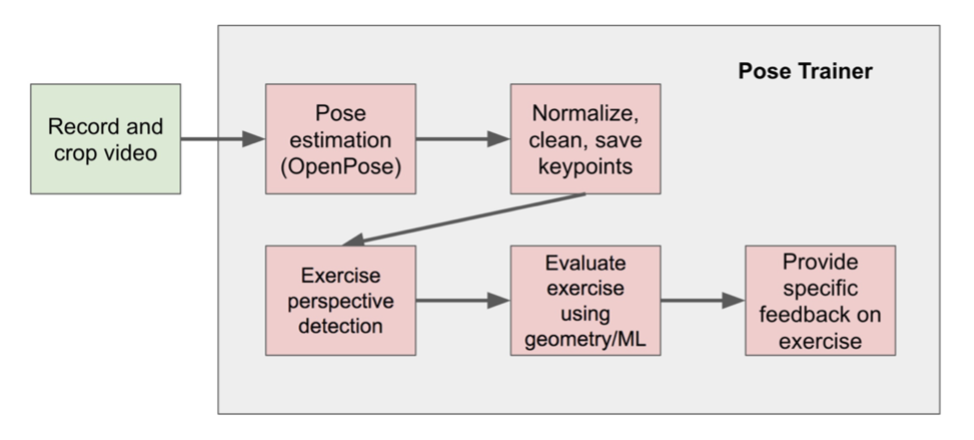
\includegraphics[width=10cm]{PoseTrainer Pipeline}
    \caption{แสดง Pipeline ของระบบ Pose Trainer}
\end{figure}

\begin{enumerate}
    \item ขั้นตอนการบันทึกวิดีโอของผู้ใช้\\
    ในขั้นตอนแรกจะเป็นการให้ผู้ใช้บันทึกวิดีโอการออกกำลังกายของตนเอง ซึ่งผู้ใช้สามารถบันทึกจากมุมใด ๆ ก็ได้ และจะไม่มีข้อจำกัดในเรื่องประเภทของกล้อง และระยะห่างของกล้อง แต่ผู้ใช้จำเป็นต้องถ่ายให้เห็นลำตัวในขณะออกกำลังกาย
    \item Pose Estimator\\
    สำหรับการตรวจจับท่าทาง ทางผู้วิจัยได้ใช้ Deep Convolutional Neural Networks (CNNs) ในการจำแนกรูปภาพ RGB ซึ่งในงานวิจัยนี้จะใช้ OpenPose เป็นโมเดลสำหรับการตรวจจับท่าทาง ซึ่งสาเหตุที่ทางผู้วิจัยได้เลือกใช้โมเดลนี้ เพราะว่า OpenPose เป็นโมเดลที่มีความแม่นยำสูงและมีประสิทธิภาพ ในขณะที่ยังสามารถต่อยอดเป็นการตรวจจับท่าทางหลาย ๆ คนพร้อมกันได้โดยที่ไม่ได้มีผลกระทบต่อประสิทธิภาพของระบบ
    \item Keypoint Normalization\\
    ผู้วิจัยได้พัฒนา parser ขึ้นเพื่อใช้กับค่า keypoint ที่ได้รับมาจากขั้นตอนที่แล้ว ในขั้นแรกจะเป็นการอ่านค่า keypoint ทั้งหมดที่ได้รับ และแยก keypoint ที่ได้ออกเป็น Part object ซึ่งจะเก็บค่า x, y และค่า confidence ของแต่ละ keypoint จากนั้นระบบจะทำการรวมแต่ละ Part object และสร้างเป็น skeleton ของตัวคนที่ได้ predict ขึ้น จากนั้นตัวระบบจะ normalize ข้อมูลท่าทางโดยยึดตามความยาวของลำตัวเป็นหน่วย pixel ซึ่งจะคำนวณได้จากค่าเฉลี่ยของความห่างระหว่าง keypoint ของส่วนคอ กับ keypoint ของส่วนสะโพก
    \item Perspective Detection\\
    ทางผู้วิจัยได้ทำการแก้ไขความกำกวมของมุมกล้องในหลาย ๆ ท่าทางการออกกำลังกาย เช่นในท่า bicep curl จะสามารถใช้แขนข้างใดก็ได้ ถ้ามุมกล้องเป็นมุมด้านข้างจะทำให้เกิดความกำกวมขึ้น ทางผู้วิจัยจึงแก้ไขโดยการวัดว่า keypoint ด้านไหนที่เห็นมากที่สุดในของทั้งวิดีโอ
    \item Geometry Evaluation\\
    ต่อไปจะทำการคำนวณ body vector จาก keypoint ที่สนใจ และได้ทำการออกแบบ geometric heuristics เพื่อนำมาวัดผลใน body vector เพื่อทำการวัดผลการออกกำลังกาย
    \item Machine Learning Evaluation\\
    การวัดผลท่าทางการออกกำลังกายอีกรูปแบบหนึ่งที่ผู้วิจัยได้นำมาใช้คือการนำ machine learning มาปรับใช้ โดยจะใช้ dynamic time warping (DWT) และ nearest neighbor classifier
\end{enumerate}

\subsubsection{ผลจากการทดลอง}
ทางผู้วิจัยได้ทำการทดลองกับ 4 ท่าทางการออกกำลังกาย คือ bicep curl, front raise, shoulder shrug, standing shoulder press ซึ่งในแต่ละท่าทางจะมีการใช้ทั้งเทคนิค geometry evaluation และ machine learning ในการวัดผลท่าทางการออกกำลังกาย
\begin{enumerate}
    \item Bicep Curl\\
    ท่า Bicep Curl ที่นำมาทดลอง ใน algorithm แบบ geometric ทางผู้วิจัยได้ใช้มุมระหว่างแขนท่อนบนและลำตัว (เพื่อวัดว่าผู้ใช้ได้หมุนข้อแขนระหว่างการออกกำลังกายหรือไม่) และ วัดมุมระหว่างแขนท่อนบนที่ทำมุมกับแขนท่อนล่าง (เพื่อวัดว่าผู้ใช้ยกได้สูงเท่าใด) จากการทดลองพบว่า algorithm นี้สามารถจำแนกการออกกำลังกายที่ถูกต้องได้ทั้งหมด และ วิดีโอที่ออกกำลังกายที่ผิดจำนวน 8\% ได้ถูกจำแนกโดย algorithm นี้ว่าเป็นการออกกำลังกายที่ไม่ถูกต้อง สำหรับ algorithm ที่ใช้ machine learning ผู้วิจัยได้แบ่ง dataset จำนวน 16 วิดีโอออกเป็น training set จำนวน 9 examples และ test set จำนวน 7 examples ซึ่งผลลัพธ์ของ DTW จะได้ค่า F1 อยู่ที่ 0.85
    \item Front Raise\\
    ท่า Front Raise เมื่อใช้ geometric algorithm จะทำการวัดการเคลื่อนที่ของหลังผู้ใช้ในแนวราบ และวัดมุมที่มากที่สุดระหว่างลำตัวและแขน สำหรับ algorithm ที่ใช้ machine learning จะแบ่ง dataset จำนวน 28 วิดีโอออกเป็น training set จำนวน 16 examples และ test set จำนวน 12 examples ซึ่งได้คะแนน F1 เป็น 1.0
    \item Shoulder Shrug\\
    ในท่า Shoulder Shrug เมื่อใช้ geometric algorithm จะวัดความเคลื่อนไหวของไหล่ผู้ใช้ และวัดมุมระหว่างแขนท่อนบนกับท่อนล่าง สำหรับ machine learning algorithm จะแบ่ง dataset จำนวน 32 วิดีโอออกเป็น training set จำนวน 19 examples และ test set จำนวน 13 examples ซึ่งได้คะแนน F1 เป็น 0.85
    \item Shoulder Press\\
    ในท่า Shoulder Press เมื่อใช้ geometric algorithm จะวัดการเคลื่อนที่ของหลังผู้ใช้โดยการนำ keypoint ของคอและสะโพกมาใช้, วัดการเคลื่อนที่ของแขนโดยใช้ keypoint ของข้อศอกและคอ และวัดมุมองศาสูงสุดที่ทำมุมระหว่างแขนท่อนบนกับท่อนล่าง สำหรับ machine learning algorithm จะแบ่ง dataset จำนวน 36 วิดีโอออกเป็น training set จำนวน 21 examples และ test set จำนวน 15 examples ซึ่งได้คะแนน F1 เป็น 0.73
\end{enumerate}

\begin{figure}
    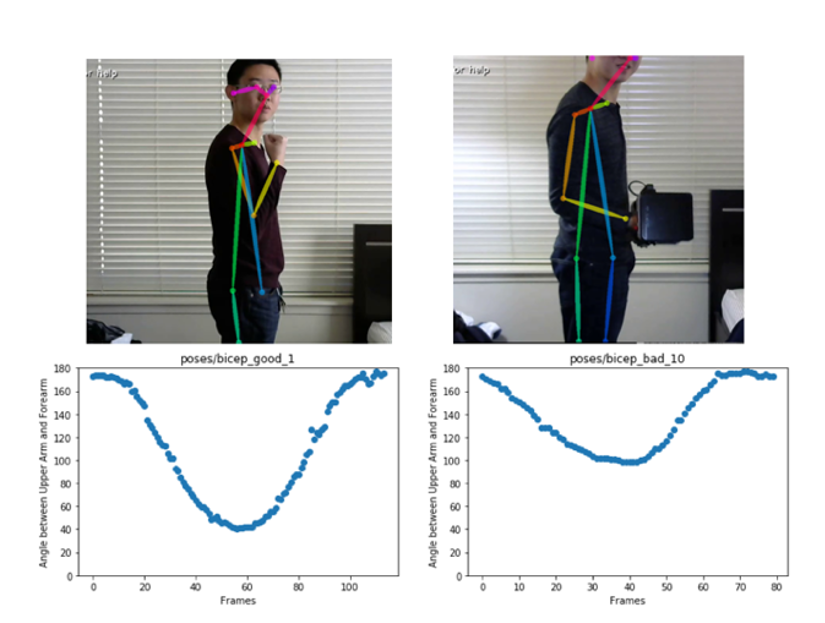
\includegraphics[width=10cm]{Bicep Curl}
    \caption{แสดงรูปภาพและกราฟองศาระหว่างแขนท่อนบนและท่อนล่างของการออกกำลังกายท่า Bicep Curl}
\end{figure}

\begin{figure}
    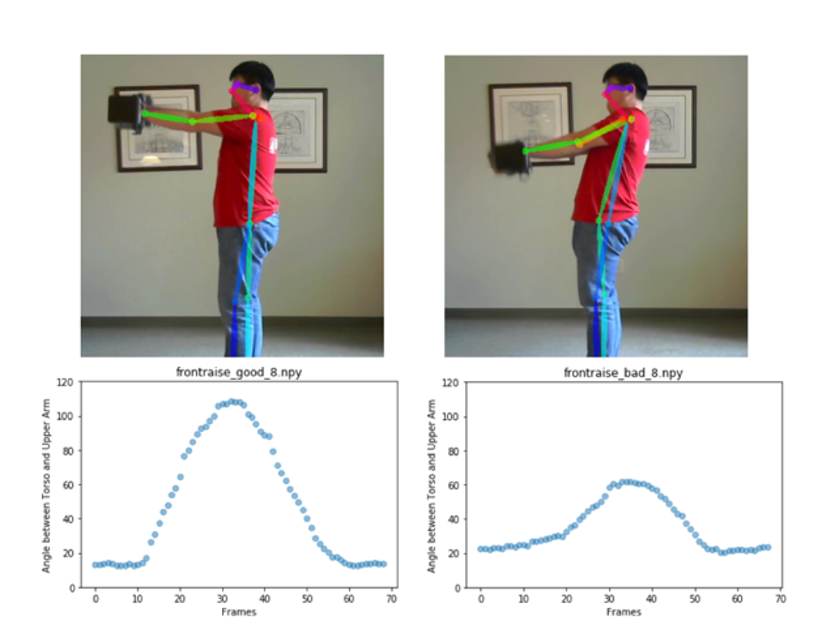
\includegraphics[width=10cm]{Front Raise}
    \caption{แสดงรูปภาพและกราฟองศาระหว่างแขนท่อนบนกับลำตัวของการออกกำลังกายท่า Front Raise}
\end{figure}

\begin{figure}
    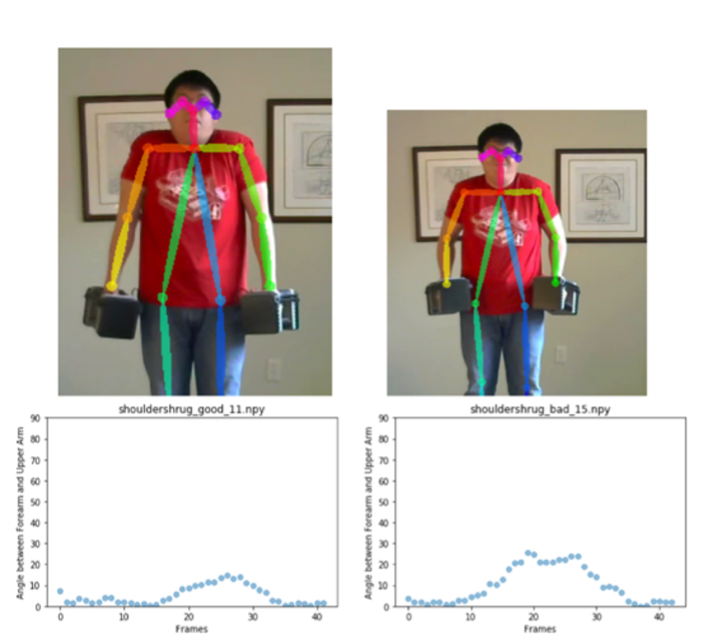
\includegraphics[width=10cm]{Shoulder Shrug}
    \caption{แสดงรูปภาพและกราฟองศาระหว่างแขนท่อนบนกับแขนท่อนล่างของการออกกำลังกายท่า Shoulder Shrug}
\end{figure}

\begin{figure}
    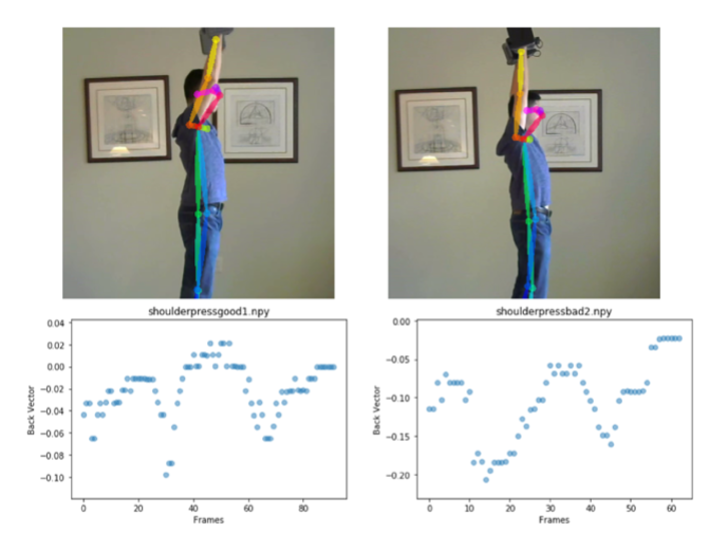
\includegraphics[width=10cm]{Shoulder Press}
    \caption{แสดงรูปภาพและกราฟการเคลื่อนที่ของหลังของการออกกำลังกายท่า Shoulder Press}
\end{figure}

\begin{figure}
    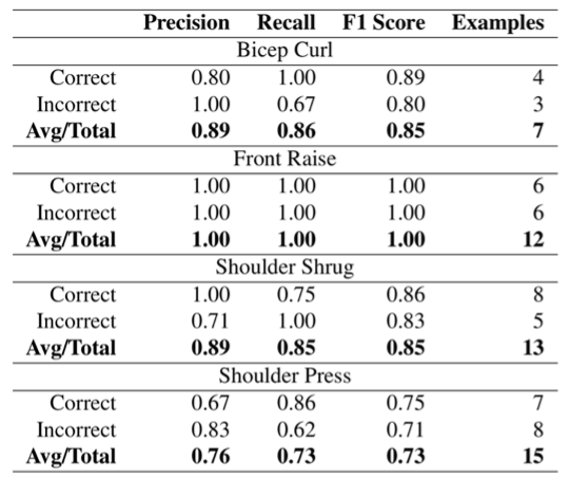
\includegraphics[width=10cm]{Post Trainer Performance}
    \caption{ตารางประสิทธิภาพและคะแนนความถูกต้องของ Machine Learning Algorithm}
\end{figure}

\subsection{Virtual Trainer with Real-Time Feedback using Kinect Sensor}
งานวิจัยการใช้ Kinect Sensor มาเป็นผู้ฝึกสอนเสมือนจริงพร้อมข้อเสนอแนะในการออกกำลังกายแบบเรียลไทม์
พร้อมมีระบบการให้คะแนนผู้ใช้เพื่อให้ผู้ใช้ได้ปรับท่าทางการออกกำลังกายได้อย่างถูกต้อง
โดยประสิทธิภาพของระบบได้ถูกประเมินโดยผู้ใช้แต่ละบุคคลที่ความแม่นยำ 96\%
โดยมี Flow Diagram ของงานวิจัยเป็นดังนี้


\begin{figure}
    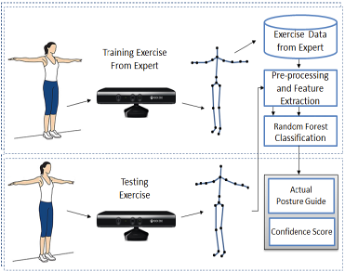
\includegraphics[width=10cm]{Virtual Trainer Flow Diagram}
    \caption{Flow Diagram ของงานวิจัย Virtual Trainer with Real-Time Feedback using Kinect Sensor}
\end{figure}

\subsubsection{หลักการที่เกี่ยวข้องในงานวิจัย}

\begin{enumerate}
    \item ในการทำงานเริ่มต้นจะแสดงระบบโต้ตอบเป็นโมเดล 3 มิติให้ผู้ใช้ได้ทำท่าทางตาม จากนั้นระบบจะแสดงคะแนนเพื่อบ่งบอกความถูกต้องของท่าทางที่ผู้ใช้ได้ออก จากการคำนวณ Random Forest (RF) Classifier ของท่าทางที่ได้ทำการฝึกไว้ และนำมาคำนวณหาค่าความเชื่อมั่น (Confidence Score)
    \item โดยก่อนที่จะทำการ Classification จะมีการทำการแปลงโครงร่างกาย 3 มิติ โดยใช้จุดกำเนิดร่วมกัน คือ
    \begin{itemize}
        \item Joint Selection: มีการเลือกข้อต่อที่ใช้เพียง 12 จุด ($J_k,k = 1, 2, 3, ..., 12$) เพื่อลดความซ้ำซ้อน และสิ่งรบกวนในบางจุดโดยใช้อัลกอริทึม evolutionary algorithm แสดงดังรูป (a)
        \item 	Angular Features: จาก Joint Selection 12 จุด ได้เป็น 8 เชิงมุม ($J_i,i = 1, 2, 3, ..., 8$) นำมาคำนวณหามุม cosine ระหว่าง 2 เวกเตอร์โดยใช้สมการ (\ref{eq:cosine}), โดยที่เวกเตอร์ X และ Y เกิดขึ้นโดยใช้ 3 ข้อต่อ แสดงดังรูป (b) และเซตของ Final Feature ($F_T$) จะประกอบด้วยเซตของ Joint Selection และ Angular Features ตามสมการ (\ref{eq:angularFeatures}) ประกอบด้วย 44 มิติ
    \end{itemize}

    \begin{equation}
        A_i = cos\alpha = \frac{\vec{X}\vec{Y}}{|X||Y|}
        \label{eq:cosine}
    \end{equation}

    \begin{equation}
        F_T = \{J_k, A_i\}
        \label{eq:angularFeatures}
    \end{equation}


    \begin{figure}
        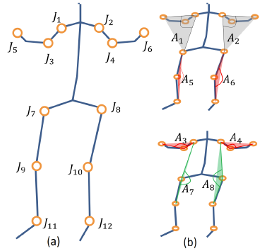
\includegraphics[width=7cm]{SelectedJointsAndAngularFeatures}
        \caption{แสดง (a) Selected joints (b) Angular features}
    \end{figure}

    \item การทำ Classification โดยการใช้หลักการ Random Forest (RF) และมีการใช้ GINI Index (GI) ในการแยกการเลือกที่วัดความไม่บริสุทธิ์ของตัวอย่างข้อมูลในคลาส โดยกำหนดให้ node t และ GI สามารถคำนวณได้โดยใช้สมการ (\ref{eq:Posterior probability}) จากนั้นตัวอย่างทดสอบจะส่งต่อไปยัง Leaf node และการ Classification จะดำเนินการโดยใช้ Posterior probability
    
    \begin{equation}
        GI(t) = 1-\sum_{x=1}^{Q}p^2(x|t)
        \label{eq:Posterior probability}
    \end{equation}
    จากสมการ (\ref{eq:Posterior probability}) $p(x│t),{x=1,2,...Q}$ หมายถึงความน่าจะเป็นของคลาสโดยประมาณสำหรับจำนวนคลาส $Q$
\end{enumerate}

แหล่งข้อมูลที่นำมาใช้ได้เลือกท่าทางการออกกำลังกายแบบพื้นฐาน 9 ท่าทาง และได้ลงทะเบียนอาสาสมัครจำนวน 10 คนมาทำการเก็บข้อมูลท่าทางการออกกำลังกาย มีการเก็บข้อมูลคนละ 9 ท่าทาง จึงได้ทั้งหมด 900 ตัวอย่าง ซึ่งพบความหลากหลายในการออกกำลังกายท่าเดียวกันแต่ออกท่าทางแตกต่างกัน
\\\indent
มีการแบ่งการเก็บ Training set และ Test set จากการลงทะเบียนอาสาสมัครทั้งหมด 10 คนที่ทำการเก็บข้อมูลท่าทางการออกกำลังกาย มีการเก็บ Training set จำนวน 4 จาก 10 คนผู้ซึ่งเป็นผู้เชี่ยวชาญด้านการออกกำลังกาย และเก็บ Test set จำนวน 6 คนที่เหลือ
\\\indent
มีการทำการเปรียบเทียบกับวิธีการอื่นที่เกี่ยวข้อง โดยใช้อุปกรณ์ Kinect เช่นเดียวกัน โดยเก็บข้อมูลจำนวน 6 คน และมีท่าทางการออกกำลังกายที่แตกต่างกัน 5 ท่าทาง  และเป็นการประมวลผลแบบ Real-time จากการเปรียบเทียบงานวิจัยนี้กับงานวิจัยที่เกี่ยวข้องนั้นพบว่างานวิจัยนี้ได้ผลความแม่นยำที่สูงกว่างานวิจัยที่นำมาเปรียบเทียบ ดังรูปที่ \ref{fig:Kinect-Compare}

\begin{figure}
    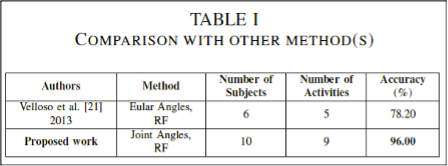
\includegraphics[height=3cm]{Kinect-Compare}
    \caption{ภาพตารางการเปรียบเทียบกับวิธีการอื่น}
    \label{fig:Kinect-Compare}
\end{figure}


\begin{table}
    \caption{ตารางเปรียบเทียบความแตกต่างของงานวิจัย}
    \begin{tabularx}{\textwidth}{ | p{4.45cm} | X | X | }
        \hline
        \textbf{หัวข้อ / งานวิจัย} & \textbf{Pose Trainer} & \textbf{Virtual Trainer with Real-Time Feedback using Kinect Sensor}\\\hline
        เทคนิคตรวจจับท่าทางที่ใช้ & ใช้โมเดล OpenPose & ใช้เทคนิค Joint Angles, Depth Sensor\\\hline
        ผลลัพธ์การตรวจจับ & ได้ผลลัพธ์ออกมาเป็น keypoint ตามจุดต่าง ๆ บนร่างกาย & ได้ผลลัพธ์เป็น keypoint ตามจุดต่าง ๆ ของร่างกาย\\\hline
        เทคนิคการวิเคราะห์ความถูกต้องของท่าทาง & Geometric, Machine Learning & Random Forest Classifier\\\hline
        ผลลัพธ์ที่ต้องการได้รับ & คำแนะนำของท่าทางการออกกำลังกาย & คะแนนความถูกต้องของท่าทาง\\\hline
        ข้อมูลที่นำมาใช้ & วิดีโอการออกกำลังกาย & ข้อมูลวิดีโอจากการเก็บข้อมูลจากอาสาสมัคร\\\hline
        รูปแบบการแบ่งข้อมูล & ขึ้นอยู่กับแต่ละท่าทาง & Training Set 4 คน, Test Set 6 คน\\\hline
        ประสิทธิภาพเชิงความถูกต้อง & ค่า F1 เท่ากับ 0.73 – 1.00 ขึ้นอยู่กับแต่ละท่าทาง & ค่า Accuracy เท่ากับ 96\%\\\hline
        จุดเด่น & เป็นระบบที่ใช้เพียงกล้องในการถ่ายวิดีโอการออกกำลังกาย  & เป็นระบบที่มีความแม่นยำสูง, ระบบเป็นแบบ Realtime\\\hline
        จุดด้อย & ระบบมีความแม่นยำน้อยกว่าอีกระบบหนึ่ง & จำเป็นต้องใช้ Kinect Sensor เพื่อใช้งานระบบนี้\\\hline
    \end{tabularx}
\end{table}
\clearpage

\section{เครื่องมือที่เกี่ยวข้อง}
\subsection{MongoDB}
MongoDB เป็น Open-Source Document Database โดยเป็นฐานข้อมูลแบบ NoSQL มีการเก็บข้อมูลเป็นแบบ JavaScript Object Notation (JSON) มีการบันทึกข้อมูลทุก ๆ Record เรียกว่า Document ซึ่งจะเก็บค่าเป็น Key และ Value และการเก็บข้อมูล Document จะถูกเก็บไว้ใน Collections (เปรียบเทียบได้กับ Table ใน Relational Database) แต่แตกต่างกันที่ Collection ไม่จำเป็นที่จะต้องมี Schema เหมือนกันก็สามารถบันทึกข้อมูลได้

% TODO: Change Pixlated MongoDB Picture
\begin{figure}
    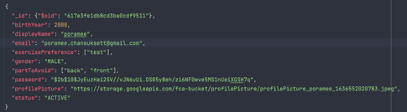
\includegraphics{mongodb example}
    \caption{ตัวอย่างโครงสร้างข้อมูลที่เก็บใน MongoDB}
\end{figure}

\subsection{Google Cloud Platform}
Google Cloud Platform คือ บริการในรูปแบบ Cloud ซึ่งจะมีผลิตภัณฑ์ที่หลากหลายโดยจะเน้นไปที่การประมวลผลแบบ Cloud และ บริการจัดเก็บไฟล์ โดยในโครงงานนี้จะใช้ผลิตภัณฑ์ 2 ตัวใน Google Cloud Platform คือ Google Cloud Functions และ Google Cloud Storage
\\\indent
Google Cloud Functions คือ บริการประมวลผลฟังก์ชันแบบไร้เซิร์ฟเวอร์ (Serverless) ซึ่งสามารถเรียกใช้ได้ผ่าน Trigger ต่าง ๆ ที่ได้กำหนดไว้ โดยในโครงงานนี้จะนำ Google Cloud Functions มาใช้สำหรับการทำ API เพื่อติดต่อกับ database และจะสามารถเรียกใช้ได้ผ่าน HTTP Request โดยเมื่อได้พัฒนา API บนเครื่องคอมพิวเตอร์โดยใช้ Node.js และ Push ขึ้น GitHub เรียบร้อยแล้ว ในโครงงานนี้จะเรียกใช้ GitHub Actions ในการ deploy ขึ้นไปยัง Google Cloud Functions โดยอัตโนมัติ
\\\indent
Google Cloud Storage คือ บริการจัดเก็บไฟล์ในรูปแบบออนไลน์ โดยใน Google Cloud Storage จะจัดเก็บในรูปแบบ object ซึ่ง object นี้จะเป็นชุดข้อมูลที่จะประกอบไปด้วยไฟล์เพียงไฟล์เดียว และ object นี้จะถูกจัดเก็บรวมกันใน container หนึ่งที่จะเรียกว่า bucket การใช้ Google Cloud Storage มีข้อดีคือสามารถตั้งค่าสิทธิ์ในการเข้าถึงไฟล์ (Permission) ได้อย่างละเอียด และสามารถใช้งานร่วมกับ Node.js ได้ดี โดยในโครงงานนี้จะใช้ Google Cloud Storage เก็บข้อมูลรูปภาพของผู้ใช้ และไฟล์คอร์สข้อมูลท่าทางการออกกำลังกาย ซึ่งในแต่ละไฟล์จะมี URL ที่สามารถเข้าถึงได้กำกับไว้ โดยที่จะจัดเก็บ URL นี้เป็น String ใน database ต่อไป

\subsection{MongoDB Atlas}
MongoDB Atlas เป็นผู้ให้บริการ MongoDB บนระบบ Cloud (MongoDB as a service) ที่ให้บริการโดยผู้พัฒนา MongoDB โดยตรง ซึ่งจะสามารถเลือก Cloud Provider สำหรับการวางระบบได้ โดยบริการนี้จะเข้ามาช่วยดูแลเรื่องการกำหนดค่าต่าง ๆ ทำให้ง่ายต่อการใช้งาน

\subsection{Node.js}
Node.js คือ Runtime Environment สำหรับฝั่ง Server ซึ่งเขียนจะด้วยภาษา JavaScript และสามารถลง Library หรือ Package อื่น ๆ เพิ่มเติมได้ ผ่าน NPM (Node Package Manager) โดยในโครงงานนี้จะนำ Node.js มาใช้งานสำหรับการพัฒนา API ซึ่งจะถูกเรียกใช้โดยแอปพลิเคชัน และจะ Deploy โดยใช้ Google Cloud Functions

\subsection{Express.js}
Express.js เป็น Web Framework ที่ใช้สำหรับการพัฒนาเว็บแอปพลิเคชันฝั่ง Backend โดย Framework นี้จะมีฟีเจอร์ที่เข้ามาช่วยในการพัฒนา API ของโครงงาน เช่น การจัดการ Routing, มีการสนับสนุน Middleware, การจัดการ Request และ Response เป็นต้น ทำให้การพัฒนาสะดวกและรวดเร็วขึ้น

\subsection{GitHub Actions}
GitHub Actions เป็นเครื่องมือของ GitHub ที่จะช่วยลดขั้นตอนการ Test และ Deploy โดยการเขียน Script เพื่อให้ GitHub Actions ทำงานให้อัตโนมัติ ซึ่งในโครงงานนี้จะนำมาใช้ในการทำ Automatic Testing และ Deploy โดยอัตโนมัติของทางฝั่ง Backend ซึ่งจะสามารถเขียน Script ให้ GitHub Actions ทำการ Build โปรแกรมและ Test อัตโนมัติเมื่อมีการ Push หรือ Merge Source Code เข้าสู่ branch ที่กำหนดไว้ได้

\subsection{ML Kit}
ML Kit เป็น Software Development Kit (SDK) สำหรับ Machine Learning บนระบบปฏิบัติการ Android และ iOS ประกอบด้วยสองส่วนหลัก คือ Base APIs และ Custom model ซึ่งสามารถใช้งานได้ทั้งแบบ Offline (On-device) และ Online (Google Cloud AI)
\\\indent
โดยในส่วนของแอปพลิเคชันที่จะนำมาใช้ในการพัฒนาโครงงานนี้คือในส่วนของ Pose Detection หรือการตรวจจับร่างกายซึ่งสามารถตรวจจับท่าทางของร่างกายแบบ Realtime จากวิดีโอต่อเนื่องหรือภาพนิ่ง โดยสามารถระบุจุดเป็น Landmark ต่าง ๆ ทั่วร่างกายทั้งหมด 33 จุด โดยจะนำค่าตำแหน่งต่าง ๆ ที่ได้รับมาวิเคราะห์หาท่าทางที่ต่างกันได้ เช่นการนำพิกัดที่แตกต่างกันมาใช้ในการนับจำนวนครั้งของการวิดพื้น หรือการนำค่าพิกัดที่แตกต่างกันมาเปรียบเทียบท่าทางการออกกำลังกายของผู้ใช้ว่าออกท่าทางได้ถูกวิธีหรือไม่
\\\indent
โดยในการใช้งาน ML Kit เดิมนั้นจะเป็นการใช้งานด้วยระบบ ML Kit for Firebase’s on-device API ซึ่งจะเป็นการส่งข้อมูลขึ้นไปประมวลผลที่ Cloud ของ Google ซึ่งจะมีข้อสังเกตคือ หากการเชื่อมต่อเครือข่ายมีความไม่เสถียร จะทำให้เกิดการ Delay ของการนำท่าทางไปวิเคราะห์ และทำให้เกิดข้อกังวลด้านความปลอดภัย เนื่องจากมีการถ่ายโอนข้อมูลไปยังเซิร์ฟเวอร์ของ Google จึงทำให้เกิดการพัฒนา ML Kit ให้สามารถทำงานได้ในรูปแบบ Offline ซึ่งจะลดปัญหาในส่วนของเครือข่าย และสร้างความมั่นใจต่อผู้ใช้งานเนื่องจากมีการประมวลผลภายในเครื่อง (Standalone) เท่านั้น และการใช้งานแบบ Standalone นั้นมีความเหมาะสมในการพัฒนาโครงงานดังกล่าวที่ต้องการความรวดเร็วในการประมวลผลท่าทาง โดยปัจจุบันทาง Google นั้นจะสนับสนุนหรืออัพเดทฟีเจอร์ใหม่ในอนาคตในระบบ ML Kit ที่เป็นรูปแบบ Standalone

\subsection{Flutter}
Flutter เป็น Cross-Platform Framework ในการพัฒนา Mobile Application พัฒนาโดย Google ซึ่งมีข้อดีคือการที่นักพัฒนาเพียงเขียนโค้ดครั้งเดียว แต่สามารถทำงานบนระบบ iOS และ Android ได้พร้อมกัน
\\\indent
Flutter สามารถใช้ทำได้หลายแพลตฟอร์ม ไม่ว่าจะเป็น iOS, Android, macOS App, Linux App, Windows App, Web และอื่น ๆ อีกมากมาย โดยโค้ดกว่า 80\% ที่เขียนจะสามารถลงทุกแพลตฟอร์มได้โดยตรง เนื่องจากสุดท้ายเราต้องมาปรับการทำงานในหน้าต่าง ๆ ให้เหมาะสมกับแพลตฟอร์มนั้น ๆ ยกตัวอย่างเช่น macOS App จะไม่มีการเรียก GPS หรือขอ Location ดังนั้นเราจำเป็นต้องปรับโค้ดให้ตรงตามข้อกำหนดดังกล่าว
\\\indent
ข้อได้เปรียบของ Flutter เมื่อเปรียบเทียบกับ Framework อื่นคือการพัฒนาจะเน้นไปในด้านประสิทธิภาพของแอปพลิเคชัน ซึ่งส่งผลให้การพัฒนาแอปพลิเคชันนั้นพัฒนาได้รวดเร็ว เพราะใช้เวลาในการ Build แอปพลิเคชันในแต่ละครั้งไม่นาน และการพัฒนาแอปพลิเคชันด้วยการใช้ Flutter ที่มีลักษณะเป็น Cross-Platform จึงทำให้ใช้งบประมาณใน\\การพัฒนาแอปพลิเคชันต่ำกว่าการพัฒนาฯ ในรูปแบบของ Native ที่เป็นการพัฒนาที่เฉพาะเจาะจงกับระบบปฏิบัติการนั้น ๆ จึงทำให้ต้นทุนในการพัฒนาสูงกว่า Cross-Platform อีกด้วย
\\\indent
เนื่องจากความเป็น Cross-Platform Framework ของ Flutter นั้นจึงทำให้แอปพลิเคชันที่พัฒนาขึ้นจะมีความลื่นไหลที่น้อยกว่าแอปพลิเคชันที่พัฒนาในรูปแบบ Native กล่าวคือ หากต้องการพัฒนาแอปพลิเคชันที่มีอัตราเฟรมที่แสดงผล 60 ภาพต่อวินาที (FPS : Frame per second) นั้นสามารถทำได้ในการพัฒนาแบบ Native แต่ไม่สามารถทำได้ใน Flutter ซึ่งในส่วนนี้จะเป็นข้อสังเกตของการพัฒนาแอปพลิเคชันด้วย Flutter หากแอปพลิเคชันที่จะพัฒนานั้นต้องการความลื่นไหลในการใช้งาน

\subsection{Microsoft Visual Studio Code}
Microsoft Visual Studio Code เป็นโปรแกรมประเภท Text Editor ถูกพัฒนาขึ้นมาโดยบริษัทไมโครซอฟต์ (Microsoft) ซึ่งสามารถแก้ไขและปรับแต่งโค้ดขนาดเล็กแต่มีประสิทธิภาพที่สูง เป็นโปรแกรมลักษณะ Open source สามารถทำงานได้หลาย Platform ทั้ง Windows, macOS และ Linux มีการสนับสนุนทั้งภาษารองรับภาษาได้หลายภาษา และมีความสามารถในการติดตั้งเครื่องมือส่วนขยายต่าง ๆ (Extension) เพื่อช่วยให้การจัดการกับโค้ดเป็นไปโดยง่าย และสามารถติดตั้งได้อย่างอิสระ

\chapter{การออกแบบและการพัฒนา}

\section{ภาพรวมของระบบ}

แอปพลิเคชันสอนออกกำลังกายที่สามารถช่วยจัดท่าทางได้อย่างถูกวิธี ผู้ใช้จะเริ่มใช้งานโดยการเข้าแอปพลิเคชันบนโทรศัพท์มือถือ และเข้าสู่ระบบด้วย Username และ Password ของตนเอง เมื่อเข้าสู่ระบบเรียบร้อยแล้วจะมีหน้าแรกให้สามารถเลือกคอร์สการออกกำลังกายได้ เมื่อผู้ใช้ทำการออกกำลังกาย ในตัวแอปพลิเคชันจะเรียกใช้งาน ML Kit ซึ่งเป็น API  เกี่ยวกับการตรวจจับท่าทาง และจะเรียกข้อมูลต่าง ๆ ที่จำเป็นในการวิเคราะห์ท่าทางจาก API ในฝั่ง Back End นอกจากนี้ฟังก์ชันอื่น ๆ ของแอปพลิเคชัน เช่น ฟังก์ชันการดูกิจกรรมและตารางคะแนนลีดเดอร์บอร์ด เป็นต้น จะมีการเรียกใช้ API นี้ด้วยเช่นกัน
\\\indent
API ในฝั่ง Back End จะอยู่ในบริการของ Google Cloud Functions ซึ่งจะมีการเรียกอ่านและเก็บข้อมูลลงใน Database โดยใช้ MongoDB และเก็บข้อมูลรูปภาพหรือไฟล์ต่าง ๆ ผ่าน Google Cloud Storage
\begin{figure}
    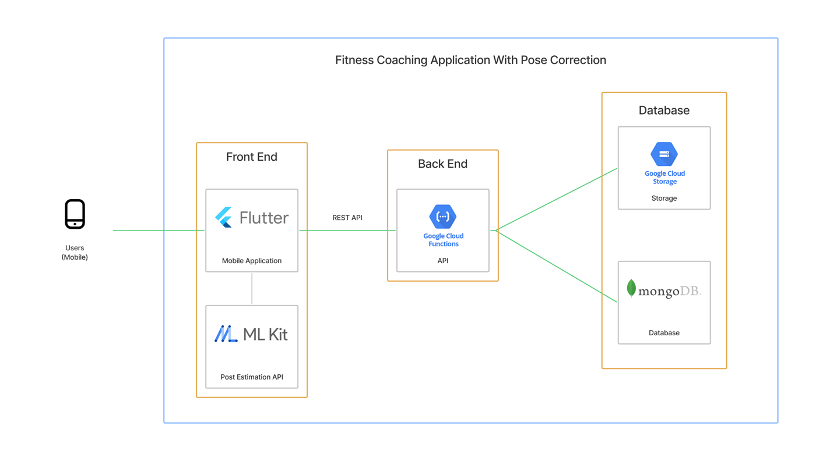
\includegraphics[width=\textwidth]{chapter_3/system overview}
    \caption{ภาพรวมระบบ}
\end{figure}

\section{แผนภาพยูสเคล (Use Case Diagram)}
\begin{figure}
    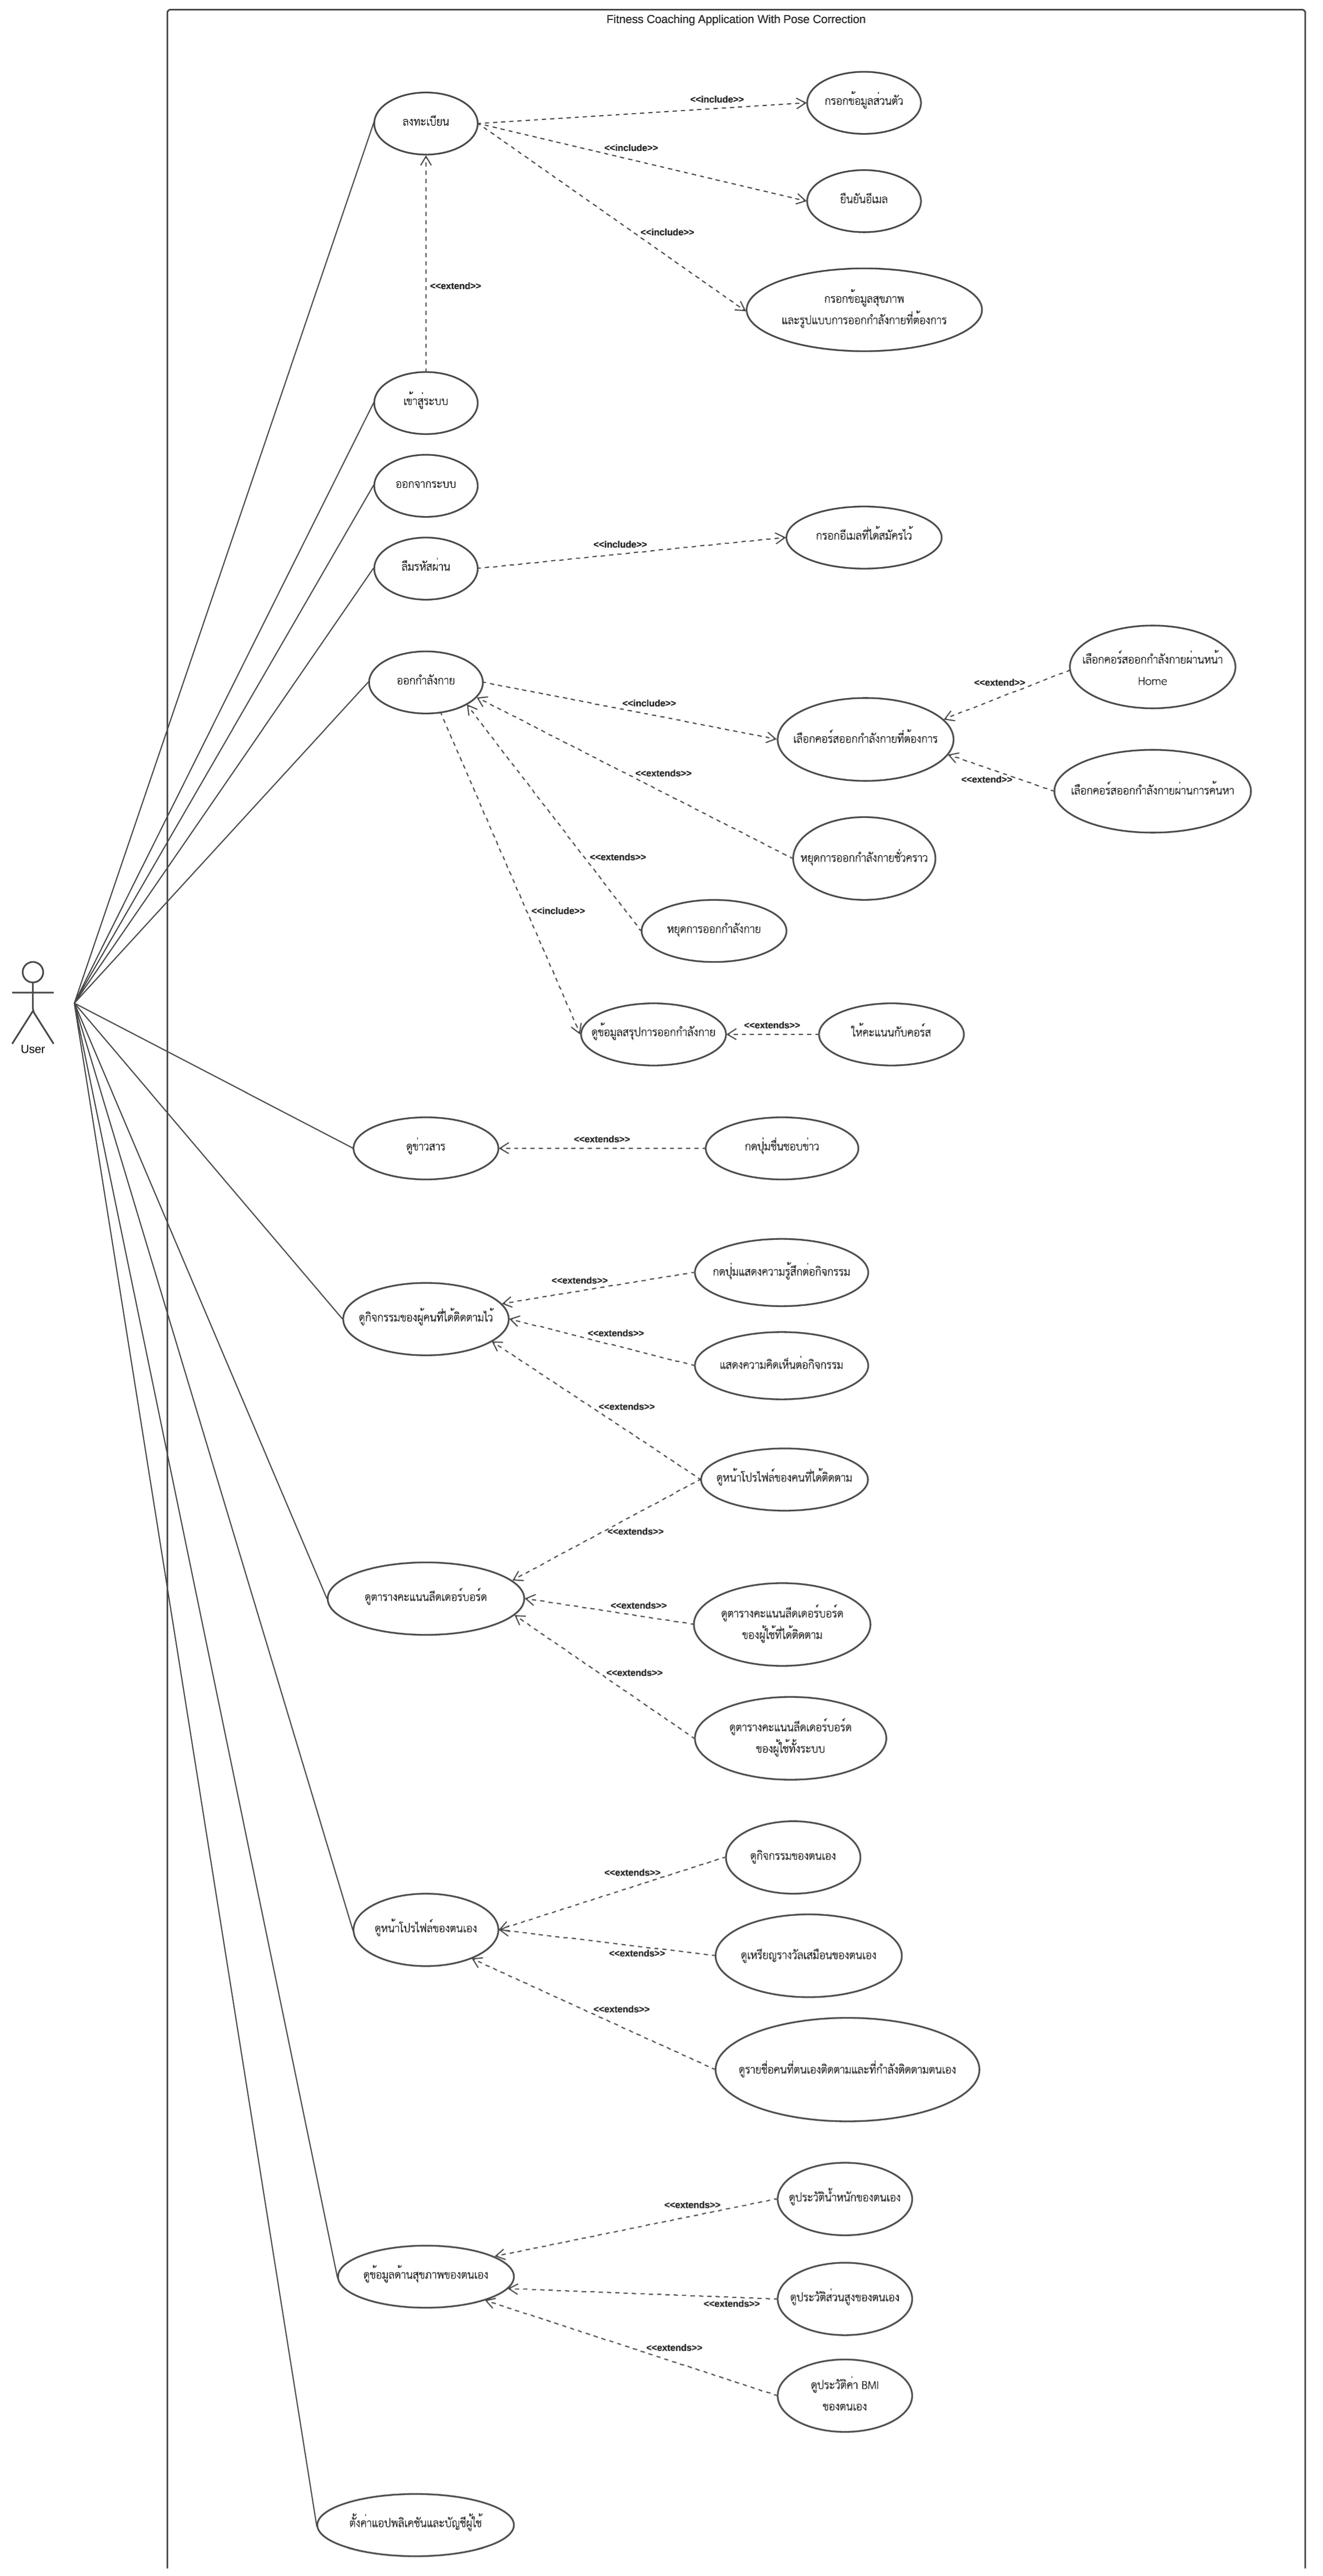
\includegraphics[height=\textheight - 3cm]{chapter_3/use case}
    \caption{แผนภาพยูสเคส}
\end{figure}
จากแผนภาพยูสเคสสามารถอธิบายได้ดังนี้
\begin{enumerate}
    \item ผู้ใช้สามารถลงทะเบียนเข้าใช้งานแอปพลิเคชันได้
    \item ผู้ใช้สามารถเข้าสู่ระบบได้
    \item ผู้ใช้สามารถออกจากระบบได้
    \item ผู้ใช้สามารถทำการกดลืมรหัสผ่านเพื่อตั้งค่ารหัสผ่านใหม่ได้
    \item ผู้ใช้สามารถเข้าสู่การออกกำลังกายได้
    \item ผู้ใช้สามารถดูข่าวสารของแอปพลิเคชันได้
    \item ผู้ใช้สามารถดูกิจกรรมของผู้คนที่ได้ติดตามไว้ได้
    \item ผู้ใช้สามารถดูตารางคะแนนลีดเดอร์บอร์ดได้
    \item ผู้ใช้สามารถดูหน้าโปรไฟล์ของตนเองได้
    \item ผู้ใช้สามารถดูข้อมูลด้านสุขภาพของตนเองได้
    \item ผู้ใช้สามารถตั้งค่าแอปพลิเคชันและตั้งค่าบัญชีผู้ใช้ได้
\end{enumerate}
\clearpage

\begin{table}
    \caption{รายละเอียด ลงทะเบียน}
    \begin{tabularx}{\textwidth}{ | >{\centering\bf} p{3cm} | X |}
        \hline
        Use Case: & ลงทะเบียน \\\hline
        Actor: & ผู้ใช้ \\\hline
        Main Flow: &
            \begin{enumerate}[table]
                \item ผู้ใช้ทำการกรอก email
                \item ผู้ใช้ทำการกรอก password ที่ต้องการ
                \item ผู้ใช้ทำการกรอก password เพื่อยืนยันอีกครั้ง
                \item ผู้ใช้ตรวจสอบการ verify email ที่ email ของตนเอง
                \item ผู้ใช้ทำการกรอก display name ที่ต้องการ
                \item ผู้ใช้ทำการเพิ่ม profile picture (สามารถข้ามได้)
            \end{enumerate}\\\hline
        Exception Flow: &
            \begin{enumerate}[table]
                \item กรณีผู้ใช้ทำการกรอก email ไม่ถูกต้องตามรูปแบบที่กำหนด แอปพลิเคชันจะแสดงข้อความว่า “Please enter a valid email”
                \item กรณีผู้ใช้ทำการกรอก password ทั้งสองช่องไม่ตรงกัน แอปพลิเคชันจะแสดงข้อความว่า “Please confirm your password”
                \item กรณีผู้ใช้ทำการกรอก password ไม่ถูกต้องตามที่เงื่อนไขกำหนด แอปพลิเคชันจะแสดงข้อความว่า “Your password must be at least 6 characters long. Please try another.”
                \item กรณีผู้ใช้ทำการกรอก display name ที่ซ้ำกันในระบบ แอปพลิเคชันจะแสดงข้อความ “This display name is already exist.”
            \end{enumerate}\\\hline
    \end{tabularx}
\end{table}


\begin{table}
    \caption{รายละเอียด เข้าสู่ระบบ}
    \begin{tabularx}{\textwidth}{ | >{\centering\bf} p{3cm} | X |}
        \hline
        Use Case: & เข้าสู่ระบบ \\\hline
        Actor: & ผู้ใช้ \\\hline
        Pre-Condition: &
        \begin{enumerate}[table]
            \item ผู้ใช้ได้เชื่อมต่ออินเทอร์เน็ต
            \item ผู้ใช้ต้องมีบัญชีผู้ใช้อยู่ในระบบ
        \end{enumerate} \\\hline
        
        Main Flow: & 
        \begin{enumerate}[table]
            \item ผู้ใช้กรอก email และ password
            \item ผู้ใช้ทำการกดปุ่มเข้าสู่ระบบ
        \end{enumerate}\\\hline
        Exception Flow: & 
        \begin{enumerate}[table]
            \item กรณีผู้ใช้ทำการกรอก email ไม่ถูกต้องตามรูปแบบที่กำหนด แอปพลิเคชันจะแสดงข้อความว่า “Please enter a valid email”
        \end{enumerate}\\\hline
    \end{tabularx}
\end{table}


\begin{table}
    \caption{รายละเอียด ออกจากระบบ}
    \begin{tabularx}{\textwidth}{ | >{\centering\bf} p{3cm} | X |}
        \hline
        Use Case: & ออกจากระบบ \\\hline
        Actor: & ผู้ใช้ \\\hline
        Pre-Condition: &
        \begin{enumerate}[table]
            \item ผู้ใช้ได้เข้าสู่ระบบเรียบร้อยแล้ว
        \end{enumerate} \\\hline
        
        Main Flow: & 
        \begin{enumerate}[table]
            \item ผู้ใช้กดปุ่มออกจากระบบ
        \end{enumerate}\\\hline
    \end{tabularx}
\end{table}

\begin{table}
    \caption{รายละเอียด ลืมรหัสผ่าน}
    \begin{tabularx}{\textwidth}{ | >{\centering\bf} p{3cm} | X |}
        \hline
        Use Case: & ลืมรหัสผ่าน \\\hline
        Actor: & ผู้ใช้ \\\hline
        Pre-Condition: &
        \begin{enumerate}[table]
            \item ผู้ใช้ได้เชื่อมต่ออินเทอร์เน็ต
            \item ผู้ใช้ต้องมีบัญชีผู้ใช้อยู่ในระบบ
        \end{enumerate} \\\hline
        
        Main Flow: & 
        \begin{enumerate}[table]
            \item ผู้ใช้กรอก email ที่ได้ทำการลงทะเบียนไว้
            \item แอปพลิเคชันส่งอีเมลเพื่อ reset รหัสผ่านไปยังผู้ใช้
            \item ผู้ใช้คลิกลิงค์เพื่อกำหนดรหัสผ่านใหม่
        \end{enumerate}\\\hline
        Exception Flow: & 
        \begin{enumerate}[table]
            \item กรณีผู้ใช้ทำการกรอก password ทั้งสองช่องไม่ตรงกัน แอปพลิเคชันจะแสดงข้อความว่า “Please confirm your password”
            \item กรณีผู้ใช้ทำการกรอก password ไม่ถูกต้องตามที่เงื่อนไขกำหนด แอปพลิเคชันจะแสดงข้อความว่า “Your password must be at least 6 characters long. Please try another.”
        \end{enumerate}\\\hline
    \end{tabularx}
\end{table}


\begin{table}
    \caption{รายละเอียด ออกกำลังกาย}
    \begin{tabularx}{\textwidth}{ | >{\centering\bf} p{3cm} | X |}
        \hline
        Use Case: & ออกกำลังกาย \\\hline
        Actor: & ผู้ใช้ \\\hline
        Pre-Condition: &
        \begin{enumerate}[table]
            \item ผู้ใช้ได้เข้าสู่ระบบเรียบร้อยแล้ว
        \end{enumerate} \\\hline
        
        Main Flow: & 
        \begin{enumerate}[table]
            \item ผู้ใช้กดเข้าหน้าหลักหรือค้นหาคอร์สออกกำลังกายเพื่อเลือกคอร์สออกกำลังกาย
            \item ผู้ใช้กดเลือกคอร์สออกกำลังกายที่ต้องการ
            \item ผู้ใช้วางโทรศัพท์มือถือ โดยให้กล้องหน้ามองเห็นร่างกายของผู้ใช้
            \item ผู้ใช้ออกกำลังกาย โดยทำตามท่าทางที่ทางแอปพลิเคชันได้สอนไว้
            \item ในระหว่างการออกกำลังกาย ผู้ใช้สามารถหยุดการออกกำลังกายชั่วคราว
            \item ในระหว่างการออกกำลังกาย ผู้ใช้สามารถหยุดการออกกำลังกาย
            \item เมื่อจบการออกกำลังกาย แอปพลิเคชันจะแสดงข้อมูลสรุปการออกกำลังกาย
            \item ผู้ใช้ให้คะแนนกับคอร์สออกกำลังกายที่ได้ออกไป
        \end{enumerate}\\\hline
        Exception Flow: & 
        \begin{enumerate}[table]
            \item เมื่อผู้ใช้ออกกำลังกายไม่ถูกต้อง แอปพลิเคชันจะมีเสียงแจ้งผู้ใช้ว่ากำลังออกกำลังกายไม่ถูกต้อง
        \end{enumerate}\\\hline
    \end{tabularx}
\end{table}


\begin{table}
    \caption{รายละเอียด หยุดการออกกำลังกายชั่วคราว}
    \begin{tabularx}{\textwidth}{ | >{\centering\bf} p{3cm} | X |}
        \hline
        Use Case: & หยุดการออกกำลังกายชั่วคราว \\\hline
        Actor: & ผู้ใช้ \\\hline
        Pre-Condition: &
        \begin{enumerate}[table]
            \item ผู้ใช้ได้เข้าสู่ระบบเรียบร้อยแล้ว
            \item ผู้ใช้อยู่ในหน้าการออกกำลังกาย
        \end{enumerate} \\\hline
        
        Main Flow: & 
        \begin{enumerate}[table]
            \item ผู้ใช้กดปุ่ม Pause เพื่อหยุดการออกกำลังกายชั่วคราว
            \item แอปพลิเคชันหยุดการจับเวลาการออกกำลังกายชั่วคราว
            \item ผู้ใช้กดปุ่ม Resume เพื่อเริ่มการออกกำลังกายต่อ
        \end{enumerate}\\\hline
    \end{tabularx}
\end{table}

\begin{table}
    \caption{รายละเอียด หยุดการออกกำลังกาย}
    \begin{tabularx}{\textwidth}{ | >{\centering\bf} p{3cm} | X |}
        \hline
        Use Case: & หยุดการออกกำลังกาย \\\hline
        Actor: & ผู้ใช้ \\\hline
        Pre-Condition: &
        \begin{enumerate}[table]
            \item ผู้ใช้ได้เข้าสู่ระบบเรียบร้อยแล้ว
            \item ผู้ใช้อยู่ในหน้าการออกกำลังกาย
        \end{enumerate} \\\hline
        
        Main Flow: & 
        \begin{enumerate}[table]
            \item ผู้ใช้กดปุ่ม Stop เพื่อหยุดการออกกำลังกาย หรือเมื่อผู้ใช้ออกกำลังกายเสร็จสิ้น
            \item แอปพลิเคชันหยุดการการออกกำลังกาย
        \end{enumerate}\\\hline
    \end{tabularx}
\end{table}

\begin{table}
    \caption{รายละเอียด ดูข่าวสาร}
    \begin{tabularx}{\textwidth}{ | >{\centering\bf} p{3cm} | X |}
        \hline
        Use Case: & ดูข่าวสาร \\\hline
        Actor: & ผู้ใช้ \\\hline
        Pre-Condition: &
        \begin{enumerate}[table]
            \item ผู้ใช้เข้าสู่ระบบเรียบร้อยแล้ว
        \end{enumerate} \\\hline
        
        Main Flow: & 
        \begin{enumerate}[table]
            \item ผู้ใช้กดปุ่มเลือกเข้าสู่หน้า News
            \item แอปพลิเคชันแสดงข้อมูลข่าวสาร
            \item ผู้ใช้เลือกอ่านข้อมูลข่าวสารที่เกี่ยวข้องกับการออกกำลังกาย ตามต้องการ
        \end{enumerate}\\\hline
    \end{tabularx}
\end{table}


\begin{table}
    \caption{รายละเอียด กดปุ่มชื่นชอบข่าว}
    \begin{tabularx}{\textwidth}{ | >{\centering\bf} p{3cm} | X |}
        \hline
        Use Case: & ดูข่าวสาร \\\hline
        Actor: & ผู้ใช้ \\\hline
        Pre-Condition: &
        \begin{enumerate}[table]
            \item ผู้ใช้ได้เข้าสู่ระบบเรียบร้อยแล้ว
            \item ผู้ใช้อยู่หน้าอ่านข้อมูลข่าวสาร          
        \end{enumerate} \\\hline
        
        Main Flow: & 
        \begin{enumerate}[table]
            \item ผู้ใช้ดูข้อมูลข่าวสาร
            \item ผู้ใช้กดปุ่มชื่นชอบข่าวสาร      
        \end{enumerate}\\\hline
    \end{tabularx}
\end{table}


\begin{table}
    \caption{รายละเอียด ดูกิจกรรมของผู้คนที่ได้ติดตามไว้}
    \begin{tabularx}{\textwidth}{ | >{\centering\bf} p{3cm} | X |}
        \hline
        Use Case: & ดูกิจกรรมของผู้คนที่ได้ติดตามไว้ \\\hline
        Actor: & ผู้ใช้ \\\hline
        Pre-Condition: &
        \begin{enumerate}[table]
            \item ผู้ใช้เข้าสู่ระบบเรียบร้อยแล้ว         
        \end{enumerate} \\\hline
        
        Main Flow: & 
        \begin{enumerate}[table]
            \item ผู้ใช้กดปุ่มเลือกเข้าสู่หน้า Activity
            \item ผู้ใช้เลือกดูกิจกรรมของผู้ใช้ที่ได้ติดตามไว้
            \item ผู้ใช้สามารถกดปุ่มแสดงความรู้สึกต่อกิจกรรม
            \item ผู้ใช้สามารถแสดงความคิดเห็นต่อกิจกรรม
            \item ผู้ใช้สามารถดูหน้าโปรไฟล์ของผู้ใช้ที่ได้ติดตามไว้
        \end{enumerate}\\\hline
    \end{tabularx}
\end{table}


\begin{table}
    \caption{รายละเอียด กดปุ่มแสดงความรู้สึกต่อกิจกรรม}
    \begin{tabularx}{\textwidth}{ | >{\centering\bf} p{3cm} | X |}
        \hline
        Use Case: & กดปุ่มแสดงความรู้สึกต่อกิจกรรม \\\hline
        Actor: & ผู้ใช้ \\\hline
        Pre-Condition: &
        \begin{enumerate}[table]
            \item ผู้ใช้ได้เข้าสู่ระบบเรียบร้อยแล้ว
            \item ผู้ใช้เลือกดูกิจกรรมของผู้ใช้ที่ได้ติดตามไว้
                   
        \end{enumerate} \\\hline
        
        Main Flow: & 
        \begin{enumerate}[table]
            \item ผู้ใช้กดปุ่มแสดงความรู้สึกต่อกิจกรรม
        \end{enumerate}\\\hline
    \end{tabularx}
\end{table}


\begin{table}
    \caption{รายละเอียด แสดงความคิดเห็นต่อกิจกรรม}
    \begin{tabularx}{\textwidth}{ | >{\centering\bf} p{3cm} | X |}
        \hline
        Use Case: & แสดงความคิดเห็นต่อกิจกรรม \\\hline
        Actor: & ผู้ใช้ \\\hline
        Pre-Condition: &
        \begin{enumerate}[table]
            \item ผู้ใช้ได้เข้าสู่ระบบเรียบร้อยแล้ว
            \item ผู้ใช้เลือกดูกิจกรรมของผู้ใช้ที่ได้ติดตามไว้      
        \end{enumerate} \\\hline
        
        Main Flow: & 
        \begin{enumerate}[table]
            \item ผู้ใช้กดแสดงความคิดเห็นต่อกิจกรรม
        \end{enumerate}\\\hline
    \end{tabularx}
\end{table}



\begin{table}
    \caption{รายละเอียด ดูตารางคะแนนลีดเดอร์บอร์ด}
    \begin{tabularx}{\textwidth}{ | >{\centering\bf} p{3cm} | X |}
        \hline
        Use Case: & ดูตารางคะแนนลีดเดอร์บอร์ด \\\hline
        Actor: & ผู้ใช้ \\\hline
        Pre-Condition: &
        \begin{enumerate}[table]
            \item ผู้ใช้ได้เข้าสู่ระบบเรียบร้อยแล้ว
            \item ผู้ใช้อยู่ในหน้า Activity
        \end{enumerate} \\\hline
        
        Main Flow: & 
        \begin{enumerate}[table]
            \item ผู้ใช้กดปุ่ม Leaderboard
            \item แอปพลิเคชันแสดงตารางคะแนนลีดเดอร์บอร์ด
            \item ผู้ใช้กดปุ่มเพื่อแสดงตารางคะแนนลีดเดอร์บอร์ดโดยจำแนกตามกลุ่มผู้ใช้ที่ได้ติดตามไว้ และกลุ่มผู้ใช้ทั้งระบบ
            \item ผู้ใช้สามารถกดดูหน้าโปรไฟล์ของผู้ใช้ที่ได้ติดตามไว้
        \end{enumerate}\\\hline
    \end{tabularx}
\end{table}



\begin{table}
    \caption{รายละเอียด ดูตารางคะแนนลีดเดอร์บอร์ดของผู้ใช้ที่ได้ติดตาม}
    \begin{tabularx}{\textwidth}{ | >{\centering\bf} p{3cm} | X |}
        \hline
        Use Case: & ดูตารางคะแนนลีดเดอร์บอร์ดของผู้ใช้ที่ได้ติดตาม \\\hline
        Actor: & ผู้ใช้ \\\hline
        Pre-Condition: &
        \begin{enumerate}[table]
            \item ผู้ใช้ได้เข้าสู่ระบบเรียบร้อยแล้ว
            \item ผู้ใช้อยู่ในหน้าแสดงตารางคะแนนลีดเดอร์บอร์ด         
        \end{enumerate} \\\hline
        
        Main Flow: & 
        \begin{enumerate}[table]
            \item ผู้ใช้กดปุ่มแสดงตารางคะแนนลีดเดอร์บอร์ดโดยจำแนกตามกลุ่มผู้ใช้ที่ได้ติดตามไว้
        \end{enumerate}\\\hline
    \end{tabularx}
\end{table}


\begin{table}
    \caption{รายละเอียด ดูตารางคะแนนลีดเดอร์บอร์ดของผู้ใช้ทั้งระบบ}
    \begin{tabularx}{\textwidth}{ | >{\centering\bf} p{3cm} | X |}
        \hline
        Use Case: & ดูตารางคะแนนลีดเดอร์บอร์ดของผู้ใช้ทั้งระบบ \\\hline
        Actor: & ผู้ใช้ \\\hline
        Pre-Condition: &
        \begin{enumerate}[table]
            \item ผู้ใช้ได้เข้าสู่ระบบเรียบร้อยแล้ว
            \item ผู้ใช้อยู่ในหน้าแสดงตารางคะแนนลีดเดอร์บอร์ด            
        \end{enumerate} \\\hline
        
        Main Flow: & 
        \begin{enumerate}[table]
            \item ผู้ใช้กดปุ่มแสดงตารางคะแนนลีดเดอร์บอร์ดโดยจำแนกตามกลุ่มผู้ใช้ทั้งระบบ
        \end{enumerate}\\\hline
    \end{tabularx}
\end{table}



\begin{table}
    \caption{รายละเอียด ดูหน้าโปรไฟล์ของตนเอง}
    \begin{tabularx}{\textwidth}{ | >{\centering\bf} p{3cm} | X |}
        \hline
        Use Case: & ดูหน้าโปรไฟล์ของตนเอง \\\hline
        Actor: & ผู้ใช้ \\\hline
        Pre-Condition: &
        \begin{enumerate}[table]
            \item ผู้ใช้ได้เข้าสู่ระบบเรียบร้อยแล้ว         
        \end{enumerate} \\\hline
        
        Main Flow: & 
        \begin{enumerate}[table]
            \item ผู้ใช้กดปุ่มเลือกเข้าสู่หน้า Profile
            \item แอปพลิเคชันแสดงข้อมูลสรุปของผู้ใช้
            \item ผู้ใช้ตรวจสอบกิจกรรมของตนเอง
            \item ผู้ใช้ตรวจสอบเหรียญรางวัลเสมือนของตนเอง
            \item ผู้ใช้ตรวจสอบรายชื่อการติดตามกับผู้ใช้อื่น
        \end{enumerate}\\\hline
    \end{tabularx}
\end{table}


\begin{table}
    \caption{รายละเอียด ดูกิจกรรมของตนเอง}
    \begin{tabularx}{\textwidth}{ | >{\centering\bf} p{3cm} | X |}
        \hline
        Use Case: & ดูกิจกรรมของตนเอง \\\hline
        Actor: & ผู้ใช้ \\\hline
        Pre-Condition: &
        \begin{enumerate}[table]
            \item ผู้ใช้ได้เข้าสู่ระบบเรียบร้อยแล้ว
            \item ผู้ใช้อยู่ในหน้า Profile 
        \end{enumerate} \\\hline
        
        Main Flow: & 
        \begin{enumerate}[table]
            \item ผู้ใช้กดปุ่มเลือกเข้าสู่หน้า Profile
            \item แอปพลิเคชันแสดงข้อมูลสรุปของผู้ใช้
            \item ผู้ใช้ตรวจสอบกิจกรรมของตนเอง
            \item ผู้ใช้ตรวจสอบเหรียญรางวัลเสมือนของตนเอง
            \item ผู้ใช้ตรวจสอบรายชื่อการติดตามกับผู้ใช้อื่น
        \end{enumerate}\\\hline
    \end{tabularx}
\end{table}


\begin{table}
    \caption{รายละเอียด ดูเหรียญรางวัลเสมือนของตนเอง}
    \begin{tabularx}{\textwidth}{ | >{\centering\bf} p{3cm} | X |}
        \hline
        Use Case: & ดูเหรียญรางวัลเสมือนของตนเอง \\\hline
        Actor: & ผู้ใช้ \\\hline
        Pre-Condition: &
        \begin{enumerate}[table]
            \item ผู้ใช้ได้เข้าสู่ระบบเรียบร้อยแล้ว
            \item ผู้ใช้อยู่ในหน้า Profile
            
        \end{enumerate} \\\hline
        
        Main Flow: & 
        \begin{enumerate}[table]
            \item ผู้ใช้กดปุ่มแสดงเหรียญรางวัลเสมือนของตนเอง
            \item ผู้ใช้ตรวจสอบเหรียญรางวัลเสมือนของตนเอง
        \end{enumerate}\\\hline
    \end{tabularx}
\end{table}


\begin{table}
    \caption{รายละเอียด ดูรายชื่อคนที่ตนเองติดตามและที่กำลังติดตามตนเอง}
    \begin{tabularx}{\textwidth}{ | >{\centering\bf} p{3cm} | X |}
        \hline
        Use Case: & ดูรายชื่อคนที่ตนเองติดตามและที่กำลังติดตามตนเอง \\\hline
        Actor: & ผู้ใช้ \\\hline
        Pre-Condition: &
        \begin{enumerate}[table]
            \item ผู้ใช้ได้เข้าสู่ระบบเรียบร้อยแล้ว
            \item ผู้ใช้อยู่ในหน้า Profile
        \end{enumerate} \\\hline
        
        Main Flow: & 
        \begin{enumerate}[table]
            \item ผู้ใช้กดข้อความ Follower เพื่อตรวจสอบรายชื่อคนที่กำลังติดตามตนเอง
            \item ผู้ใช้กดข้อความ Following เพื่อตรวจสอบรายชื่อคนที่ตนเองติดตาม
            \item แอปพลิเคชันแสดงรายชื่อคนที่ตนเองติดตามและที่กำลังติดตามตนเอง
            \item ผู้ใช้ตรวจสอบรายชื่อคนที่ตนเองติดตามและที่กำลังติดตามตนเอง
        \end{enumerate} \\\hline
    \end{tabularx}
\end{table}


\begin{table}
    \caption{รายละเอียด ดูข้อมูลด้านสุขภาพของตนเอง}
    \begin{tabularx}{\textwidth}{ | >{\centering\bf} p{3cm} | X |}
        \hline
        Use Case: & ดูข้อมูลด้านสุขภาพของตนเอง \\\hline
        Actor: & ผู้ใช้ \\\hline
        Pre-Condition: &
        \begin{enumerate}[table]
            \item ผู้ใช้ได้เข้าสู่ระบบเรียบร้อยแล้ว
            \item ผู้ใช้อยู่ในหน้า Profile            
        \end{enumerate} \\\hline
        
        Main Flow: & 
        \begin{enumerate}[table]
            \item ผู้ใช้กดปุ่ม Health Stats
            \item แอปพลิเคชันแสดงหน้า Health Stats ซึ่งแสดงข้อมูลด้านสุขภาพ (จำนวนนาทีการออกกำลังกาย, น้ำหนัก, ส่วนสูง, ค่า BMI) ของตนเอง
            \item ผู้ใช้ตรวจสอบข้อมูลด้านสุขภาพของตนเอง  
        \end{enumerate}\\\hline
    \end{tabularx}
\end{table}


\begin{table}
    \caption{รายละเอียด ดูประวัติน้ำหนักของตนเอง}
    \begin{tabularx}{\textwidth}{ | >{\centering\bf} p{3cm} | X |}
        \hline
        Use Case: & ดูประวัติน้ำหนักของตนเอง \\\hline
        Actor: & ผู้ใช้ \\\hline
        Pre-Condition: &
        \begin{enumerate}[table]
            \item ผู้ใช้ได้เข้าสู่ระบบเรียบร้อยแล้ว
            \item ผู้ใช้อยู่ในหน้า Health Stats          
        \end{enumerate} \\\hline
        
        Main Flow: & 
        \begin{enumerate}[table]
            \item ผู้ใช้กดปุ่ม Weight
            \item แอปพลิเคชันแสดงข้อมูลสถิติของค่าน้ำหนักของผู้ใช้ที่ได้บันทึกไว้ โดยแสดงเป็นกราฟเส้นและค่าที่ได้บันทึกไว้
            \item ผู้ใช้ตรวจสอบสถิติค่าน้ำหนักของตนเอง
        \end{enumerate}\\\hline
    \end{tabularx}
\end{table}



\begin{table}
    \caption{รายละเอียด ดูประวัติส่วนสูงของตนเอง}
    \begin{tabularx}{\textwidth}{ | >{\centering\bf} p{3cm} | X |}
        \hline
        Use Case: & ดูประวัติส่วนสูงของตนเอง \\\hline
        Actor: & ผู้ใช้ \\\hline
        Pre-Condition: &
        \begin{enumerate}[table]
            \item ผู้ใช้ได้เข้าสู่ระบบเรียบร้อยแล้ว
            \item ผู้ใช้อยู่ในหน้า Health Stats          
        \end{enumerate} \\\hline
        
        Main Flow: & 
        \begin{enumerate}[table]
            \item ผู้ใช้กดปุ่ม Height
            \item แอปพลิเคชันแสดงข้อมูลสถิติของค่าส่วนสูงของผู้ใช้ที่ได้บันทึกไว้ โดยแสดงเป็นกราฟเส้นและค่าที่ได้บันทึกไว้
            \item ผู้ใช้ตรวจสอบสถิติค่าส่วนสูงของตนเอง   
        \end{enumerate}\\\hline
    \end{tabularx}
\end{table}


\begin{table}
    \caption{รายละเอียด ดูประวัติค่า BMI ของตนเอง}
    \begin{tabularx}{\textwidth}{ | >{\centering\bf} p{3cm} | X |}
        \hline
        Use Case: & ดูประวัติค่า BMI ของตนเอง \\\hline
        Actor: & ผู้ใช้ \\\hline
        Pre-Condition: &
        \begin{enumerate}[table]
            \item ผู้ใช้ได้เข้าสู่ระบบเรียบร้อยแล้ว
            \item ผู้ใช้อยู่ในหน้า Health Stats
        \end{enumerate} \\\hline
        
        Main Flow: & 
        \begin{enumerate}[table]
            \item ผู้ใช้กดปุ่ม BMI
            \item แอปพลิเคชันแสดงข้อมูลสถิติของค่า BMI ของผู้ใช้ที่แอปพลิเคชันคำนวณมาจากค่าน้ำหนักและส่วนสูงที่ผู้ใช้ได้บันทึกไว้
            \item ผู้ใช้ตรวจสอบสถิติค่า BMI ของตนเอง
        \end{enumerate}\\\hline
    \end{tabularx}
\end{table}



\begin{table}
    \caption{รายละเอียด ตั้งค่าแอปพลิเคชันและบัญชีผู้ใช้}
    \begin{tabularx}{\textwidth}{ | >{\centering\bf} p{3cm} | X |}
        \hline
        Use Case: & ตั้งค่าแอปพลิเคชันและบัญชีผู้ใช้ \\\hline
        Actor: & ผู้ใช้ \\\hline
        Pre-Condition: &
        \begin{enumerate}[table]
            \item ผู้ใช้ได้เข้าสู่ระบบเรียบร้อยแล้ว
            \item ผู้ใช้อยู่ในหน้า Profile            
        \end{enumerate} \\\hline
        
        Main Flow: & 
        \begin{enumerate}[table]
            \item ผู้ใช้กดปุ่ม Settings
            \item แอปพลิเคชันแสดงหน้า Settings ในการตั้งค่าแอปพลิเคชันและบัญชีผู้ใช้
            \item ผู้ใช้ตรวจสอบการตั้งค่าแอปพลิเคชันและบัญชีผู้ใช้
            \item ผู้ใช้กำหนดค่าของการตั้งค่าแอปพลิเคชันและบัญชีผู้ใช้            
        \end{enumerate}\\\hline
    \end{tabularx}
\end{table}
\clearpage

\section{แผนผังการทำงานแบบลำดับปฏิสัมพันธ์ (Sequence Diagram)}
การออกแบบแผนผังการทำงานแบบลำดับปฏิสัมพันธ์ ดังนี้

\begin{figure}
    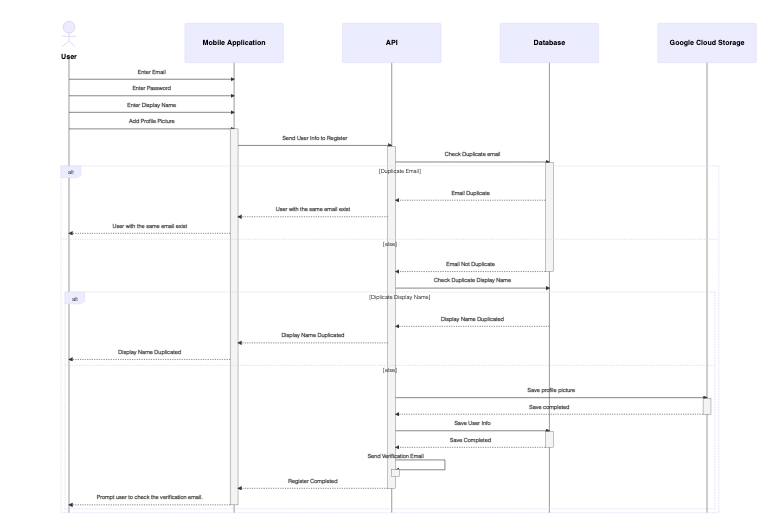
\includegraphics[width=\textwidth]{chapter_3/sequence/Register-1.md.png}
    \caption{การทำงานในส่วนการลงทะเบียนผู้ใช้}
\end{figure}

\begin{figure}
    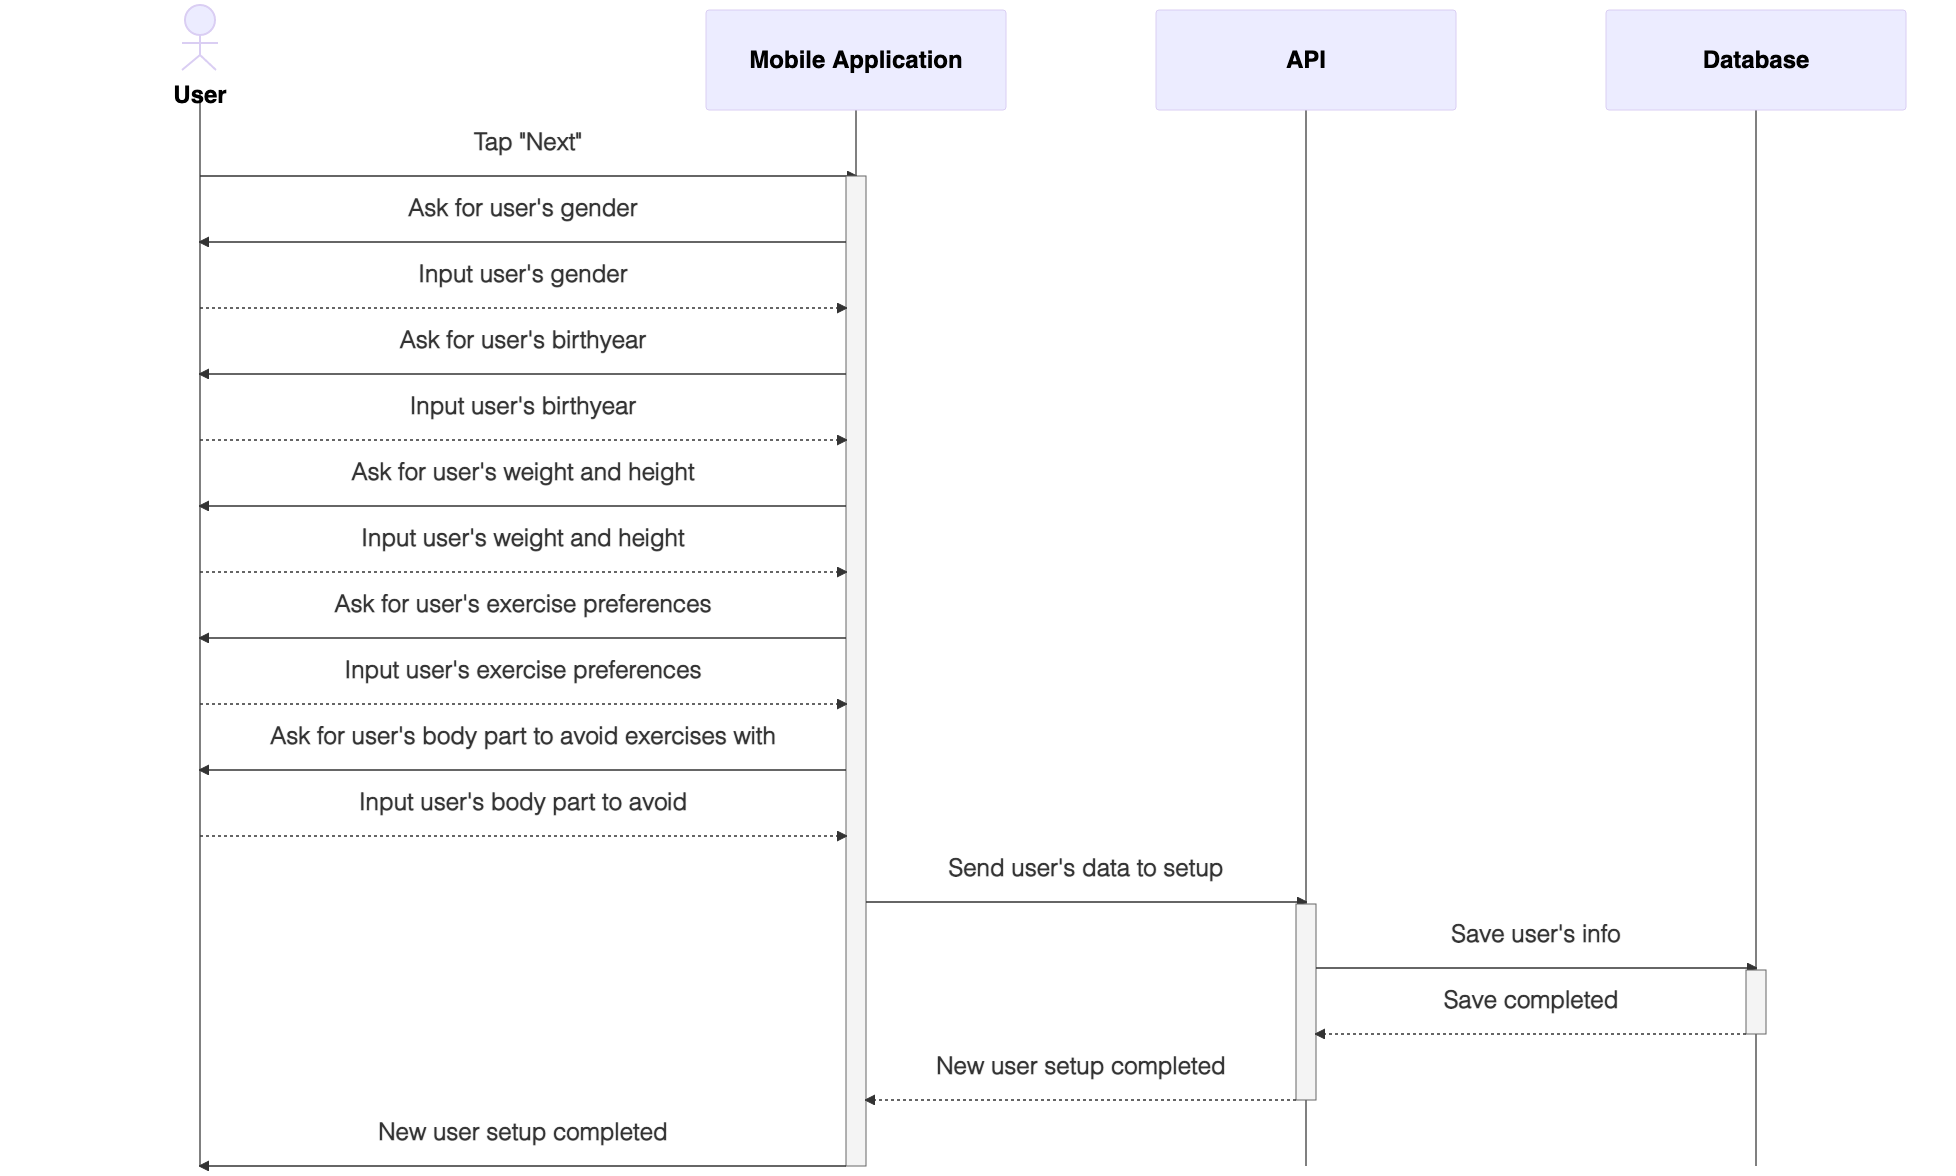
\includegraphics[width=\textwidth]{chapter_3/sequence/New User Setup-1.md.png}
    \caption{การทำงานในส่วนการตอบคำถามความต้องการออกกำลังกาย}
\end{figure}

\begin{figure}
    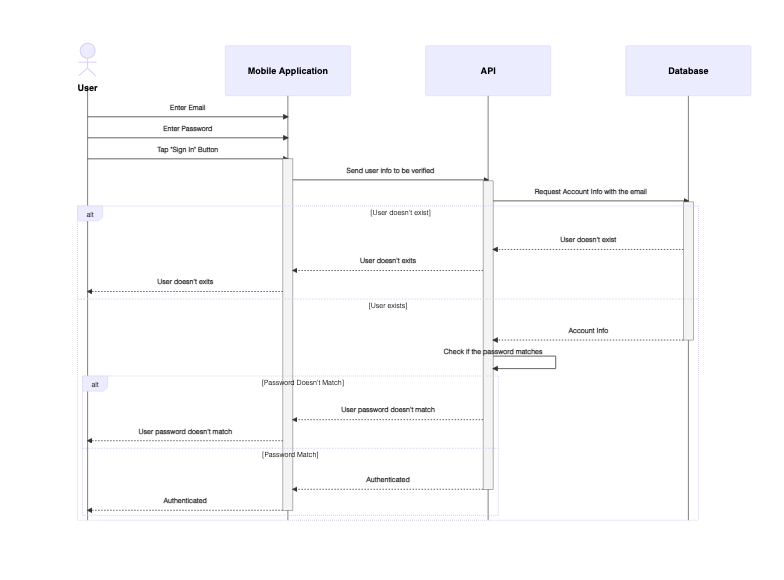
\includegraphics[width=\textwidth]{chapter_3/sequence/Sign In-1.md.png}
    \caption{การทำงานในส่วนการเข้าสู่ระบบ}
\end{figure}

\begin{figure}
    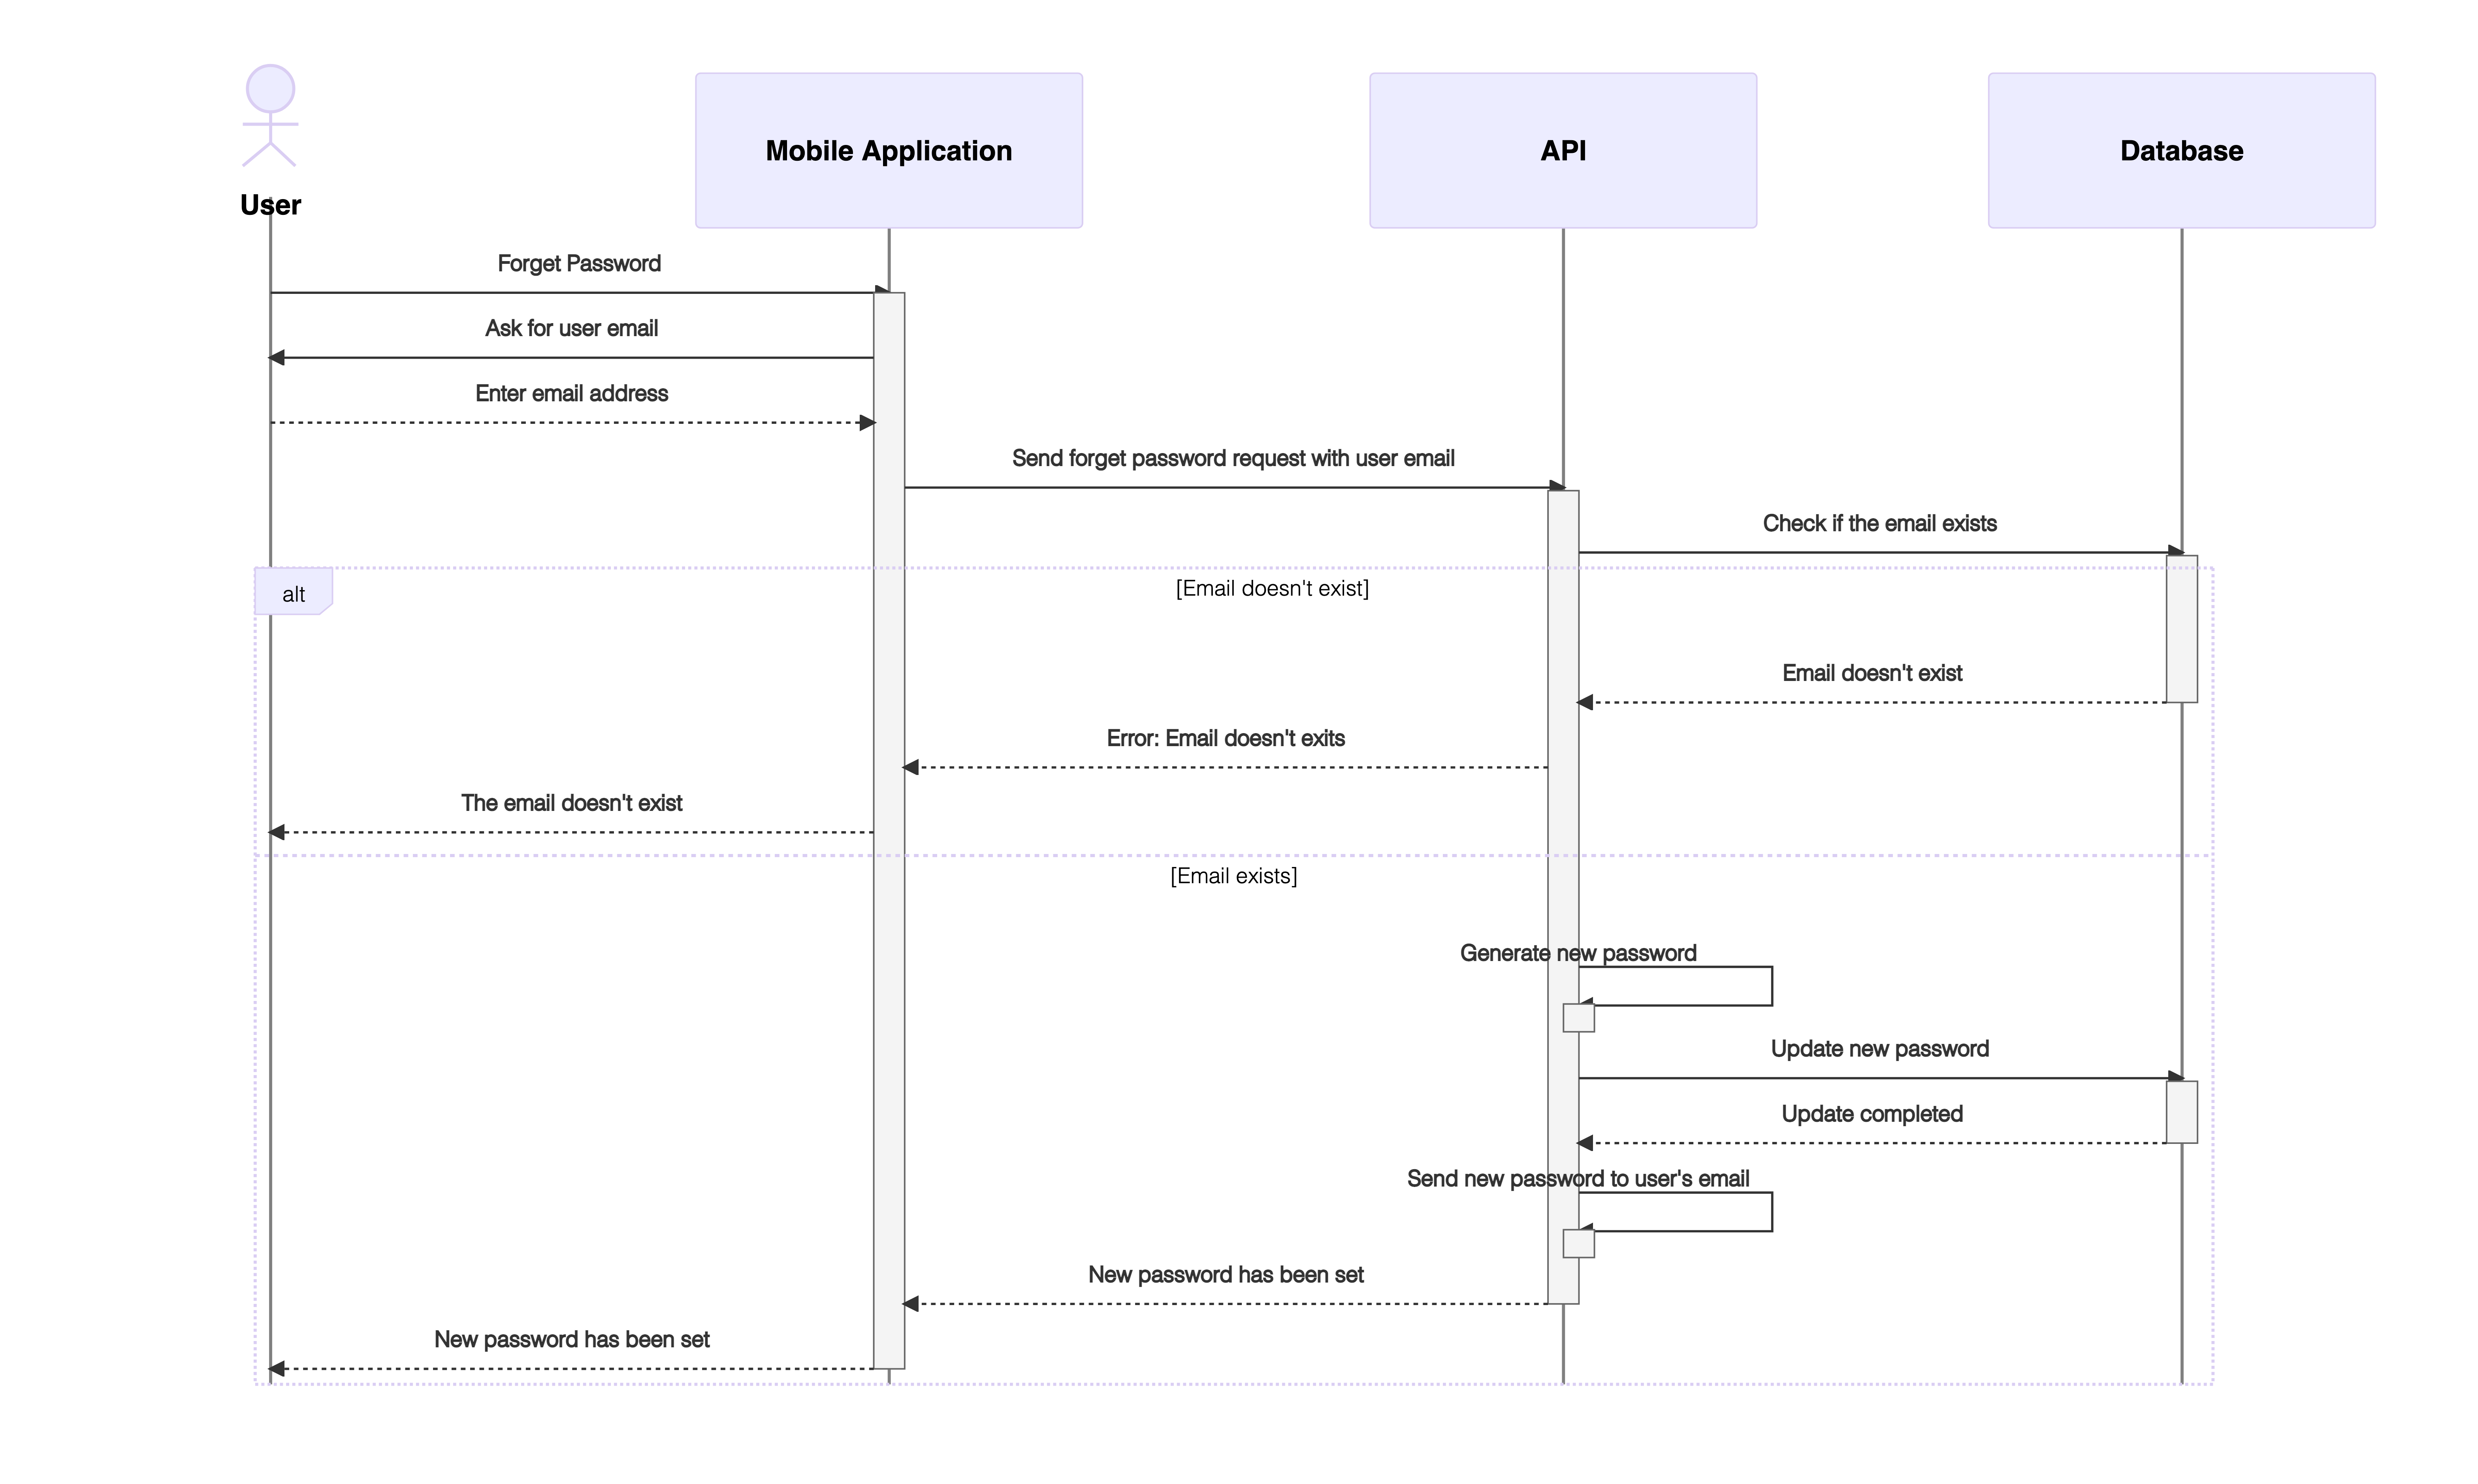
\includegraphics[width=\textwidth]{chapter_3/sequence/Forget Password-1.md.png}
    \caption{การทำงานในส่วนการลืมรหัสผ่าน}
\end{figure}

\begin{figure}
    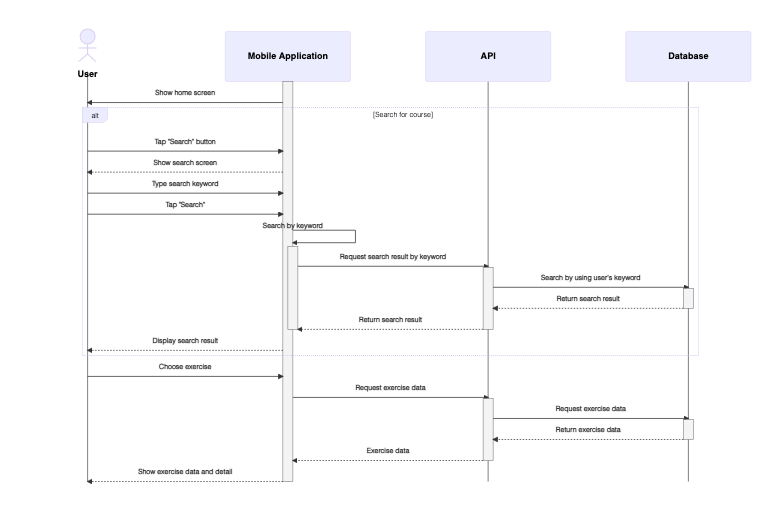
\includegraphics[width=\textwidth]{chapter_3/sequence/Exercise Course Selection-1.md.png}
    \caption{การทำงานในส่วนการเลือกคอร์สออกกำลังกาย}
\end{figure}

\begin{figure}
    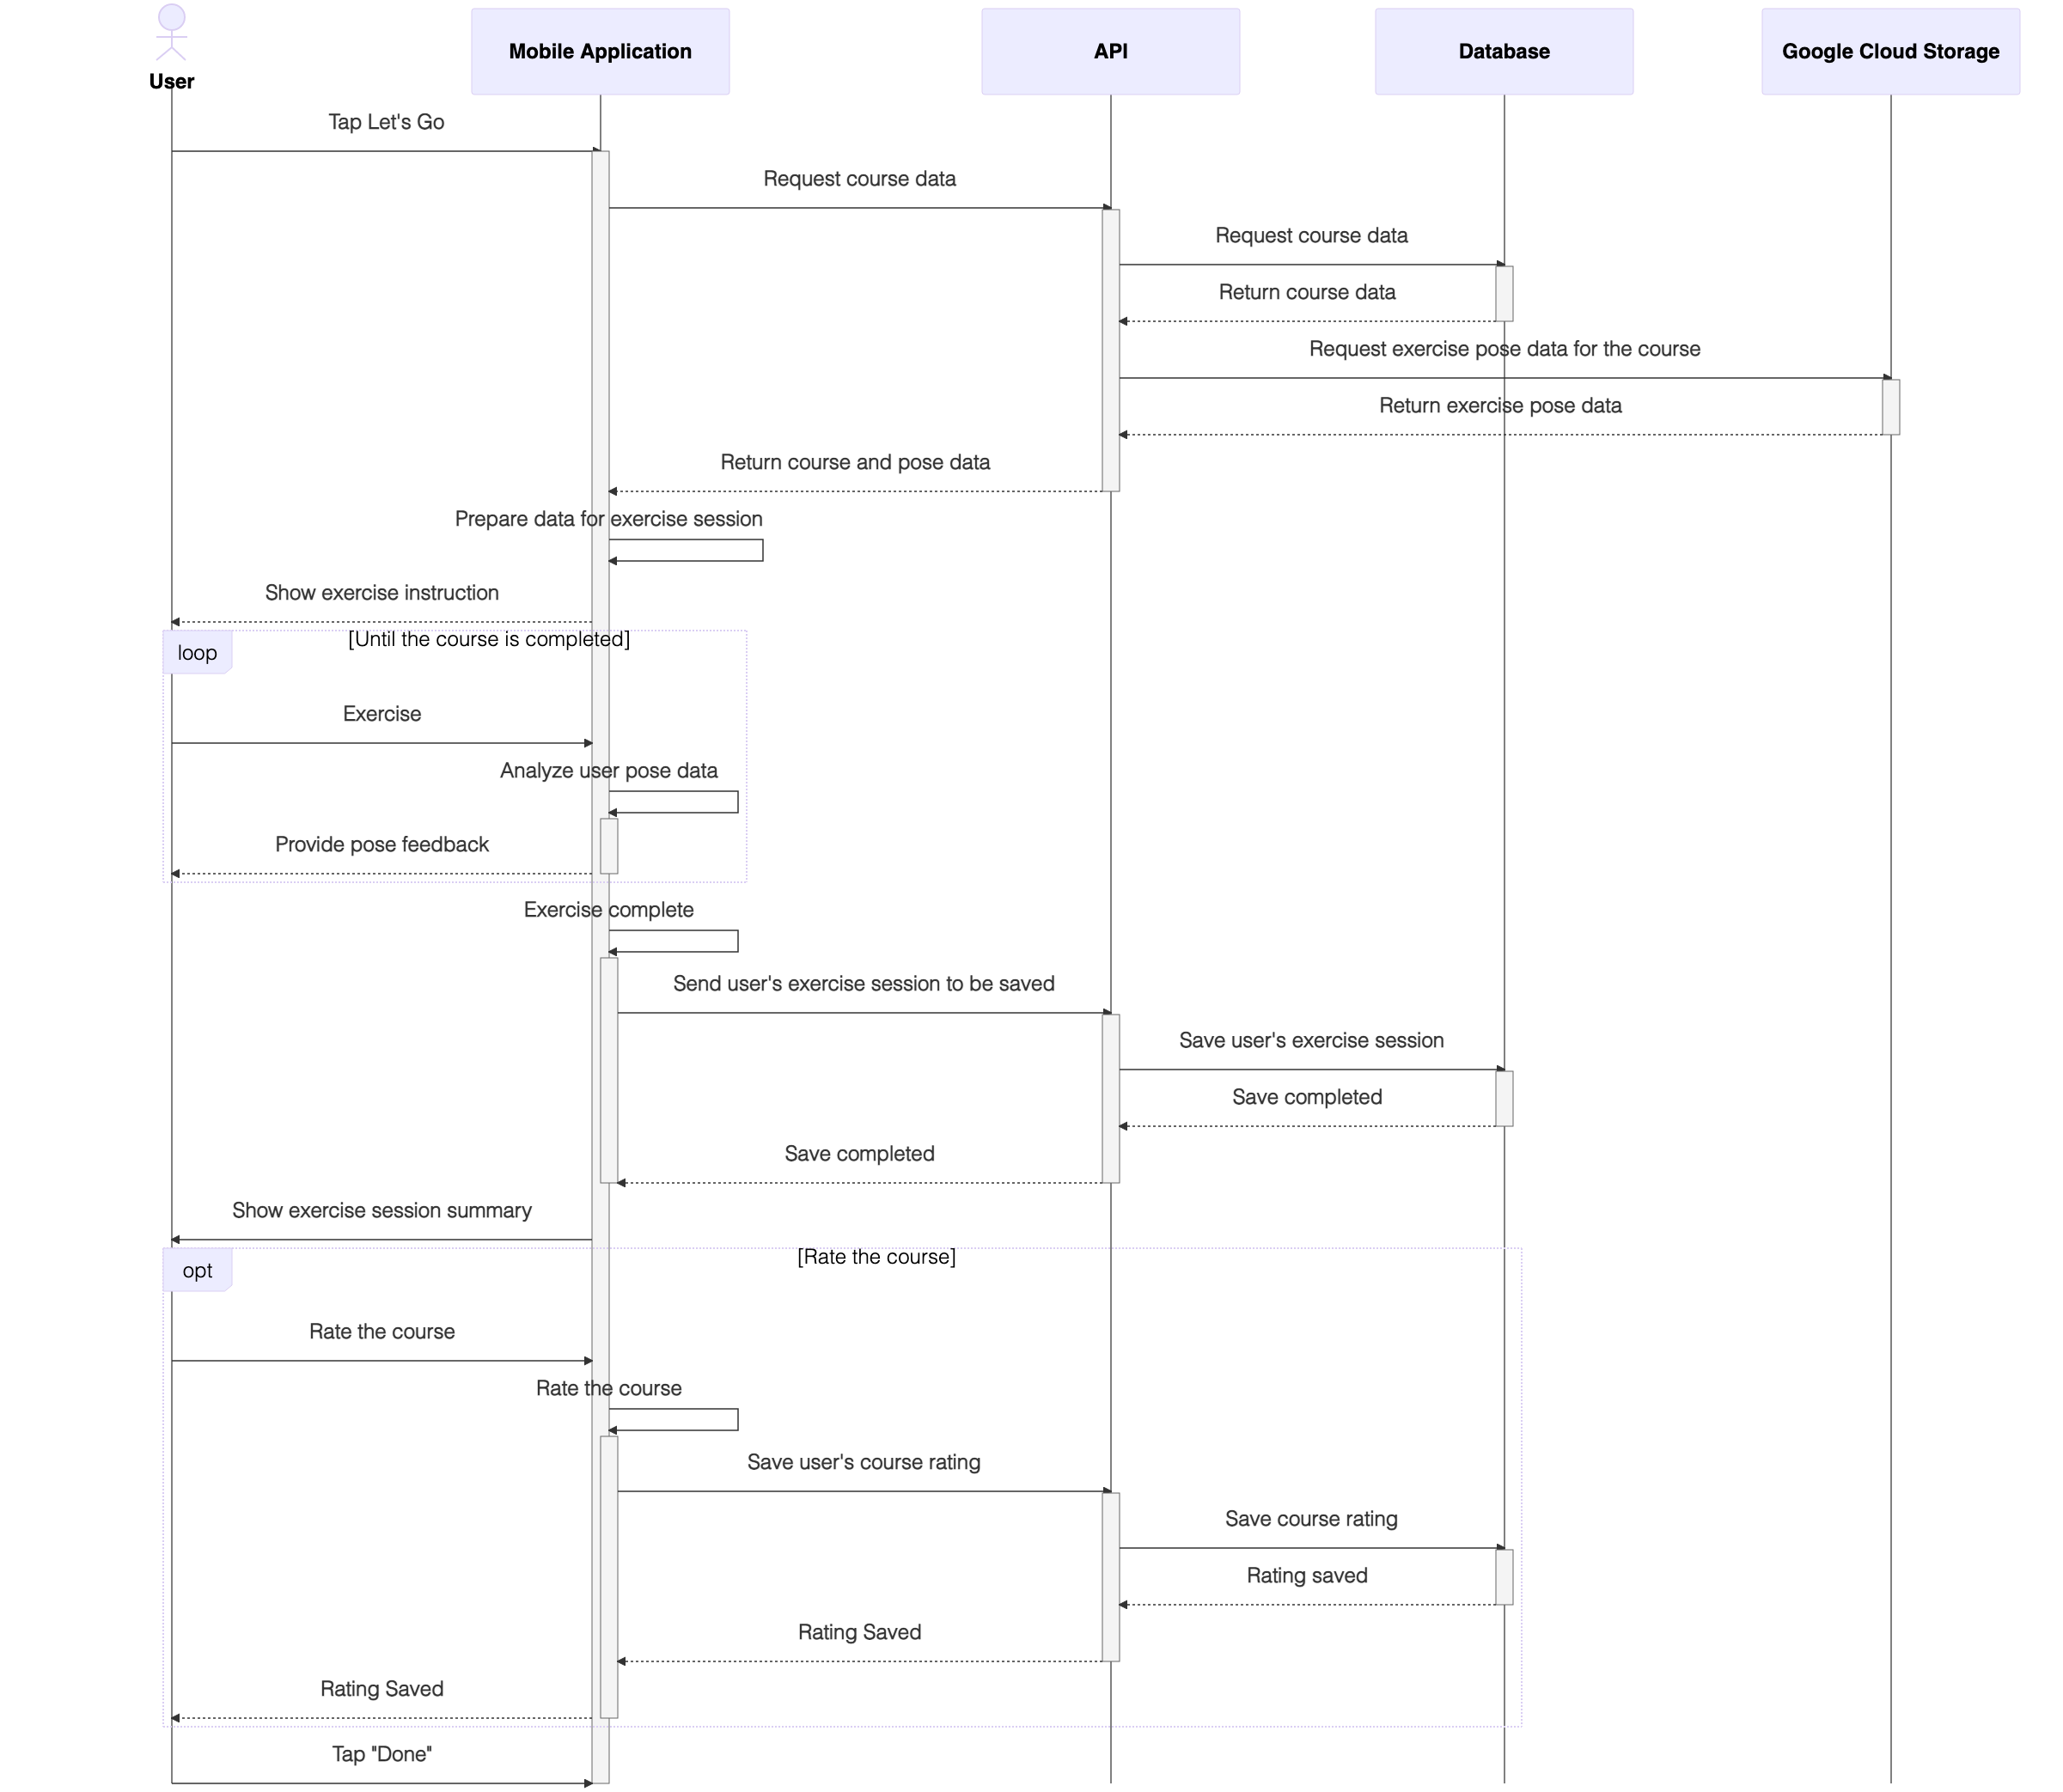
\includegraphics[width=\textwidth]{chapter_3/sequence/Exercise-1.md.png}
    \caption{การทำงานในส่วนการออกกำลังกาย}
\end{figure}

\begin{figure}
    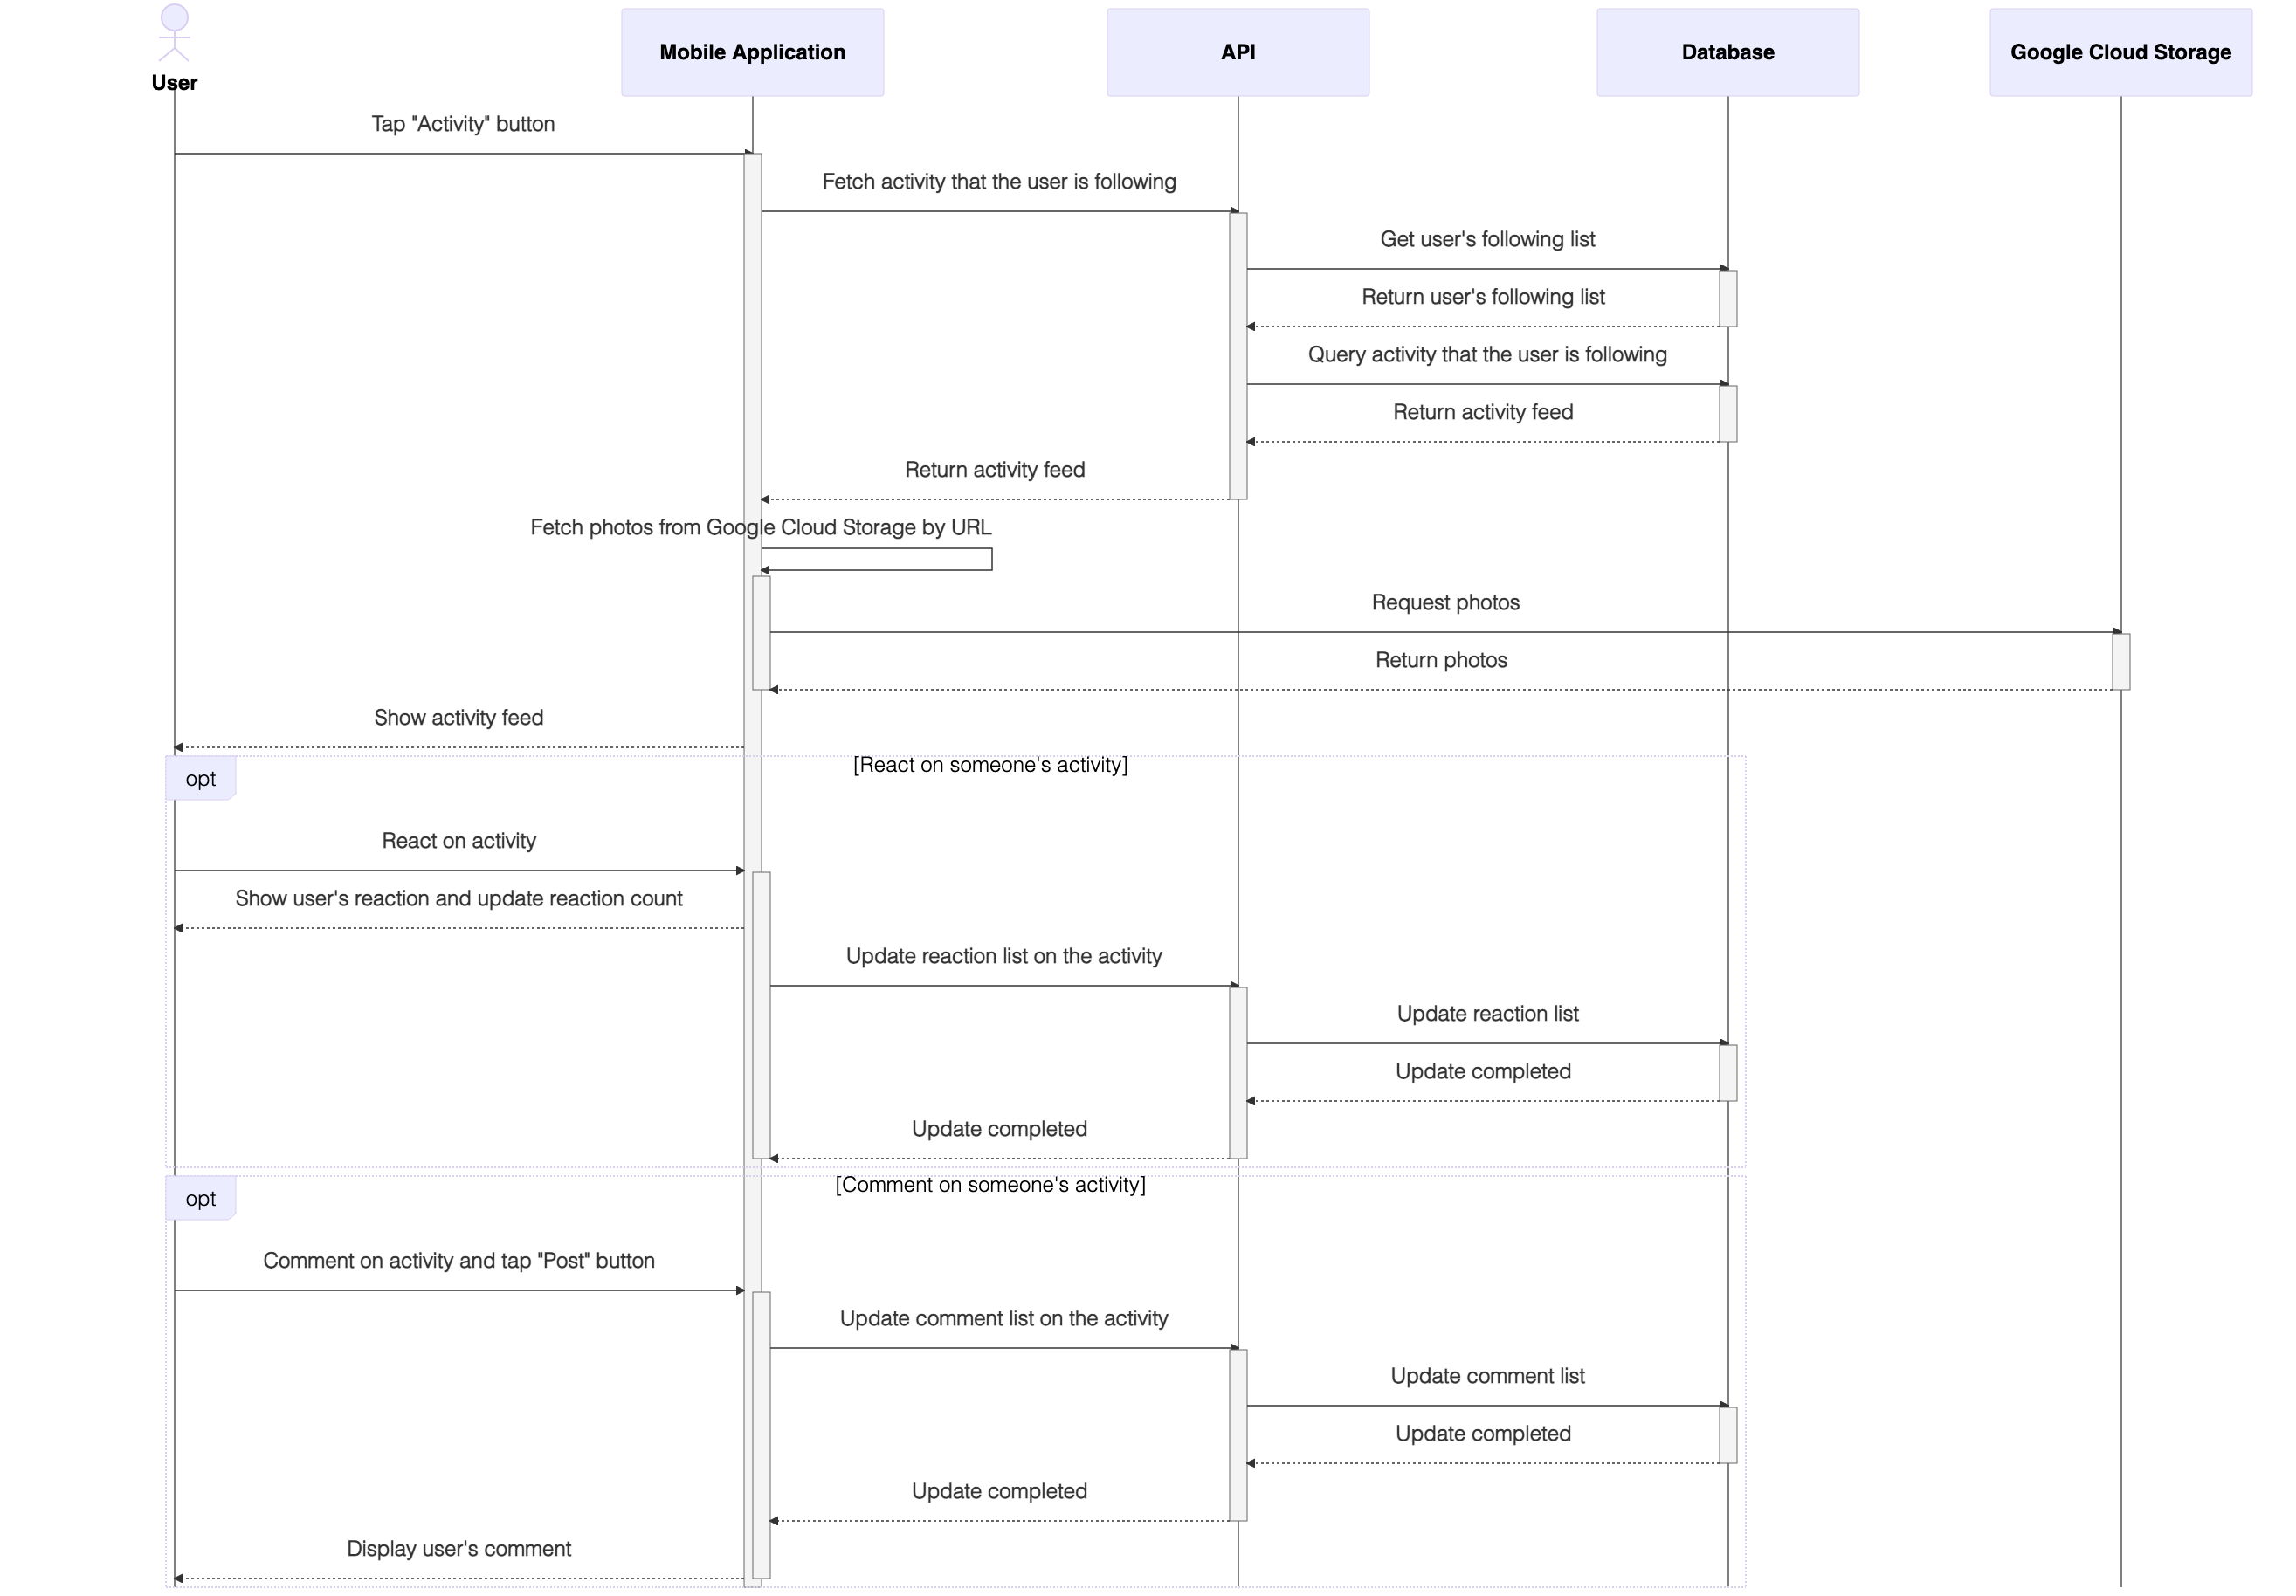
\includegraphics[width=\textwidth]{chapter_3/sequence/Activity-1.md.png}
    \caption{การทำงานในส่วนกิจกรรมของผู้ใช้}
\end{figure}

\begin{figure}
    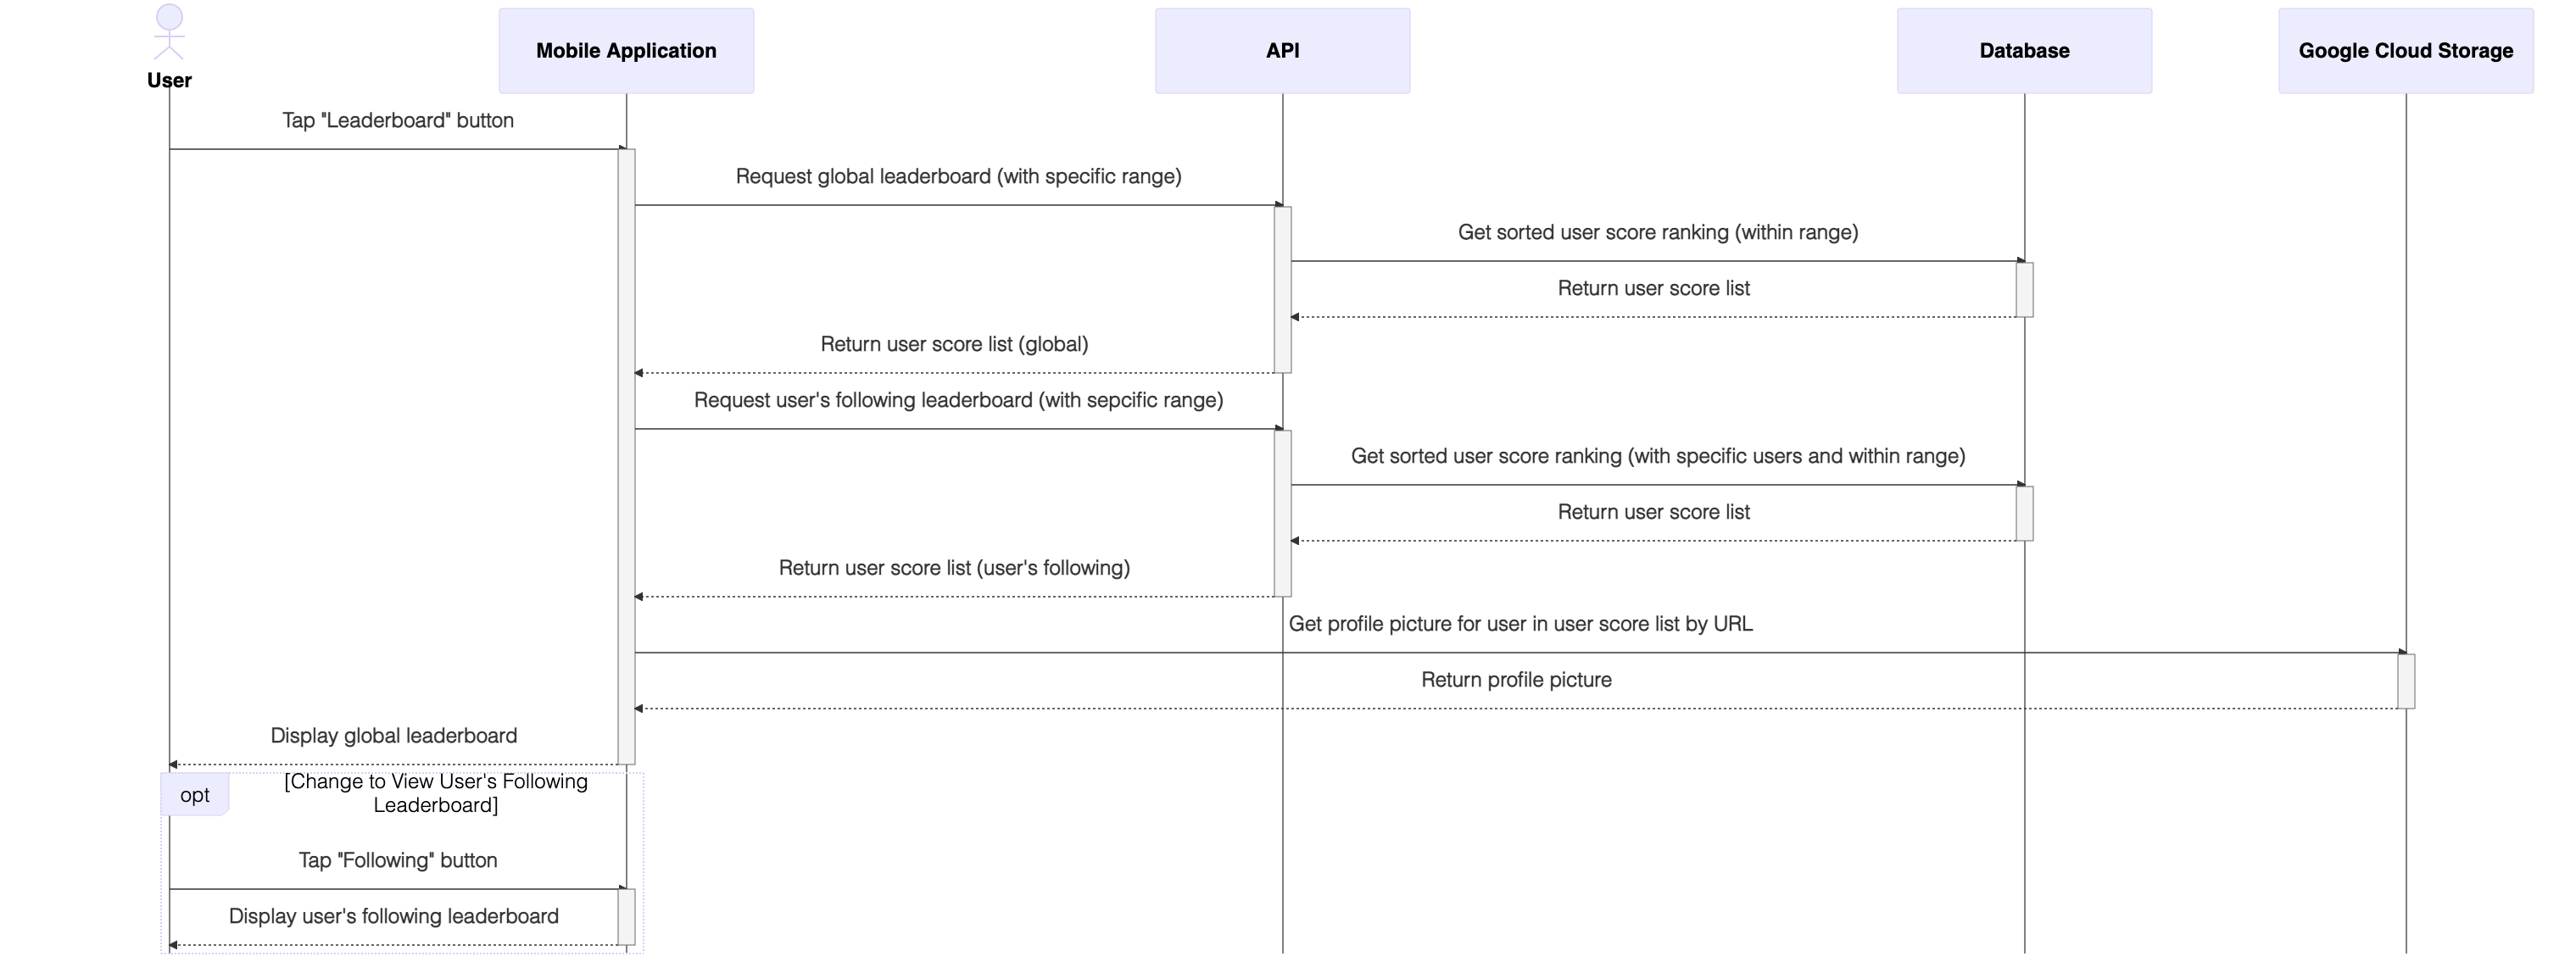
\includegraphics[width=\textwidth]{chapter_3/sequence/Leaderboard-1.md.png}
    \caption{การทำงานในส่วนตารางคะแนน Leaderboard}
\end{figure}

\begin{figure}
    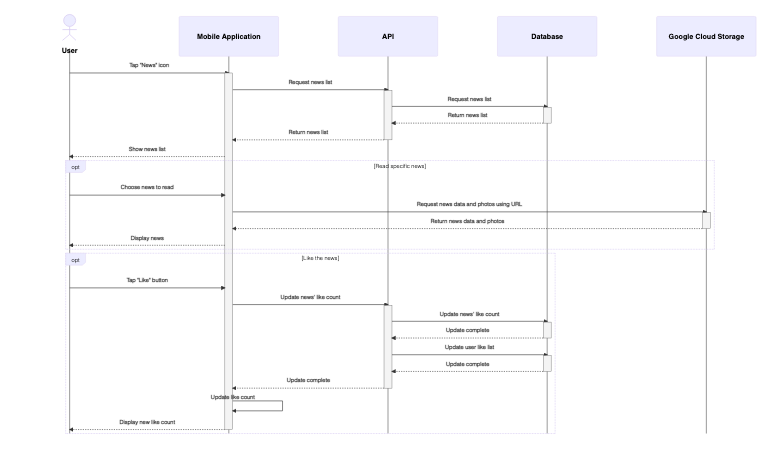
\includegraphics[width=\textwidth]{chapter_3/sequence/News-1.md.png}
    \caption{การทำงานในส่วนข้อมูลข่าวสารของแอปพลิเคชัน}
\end{figure}

\begin{figure}
    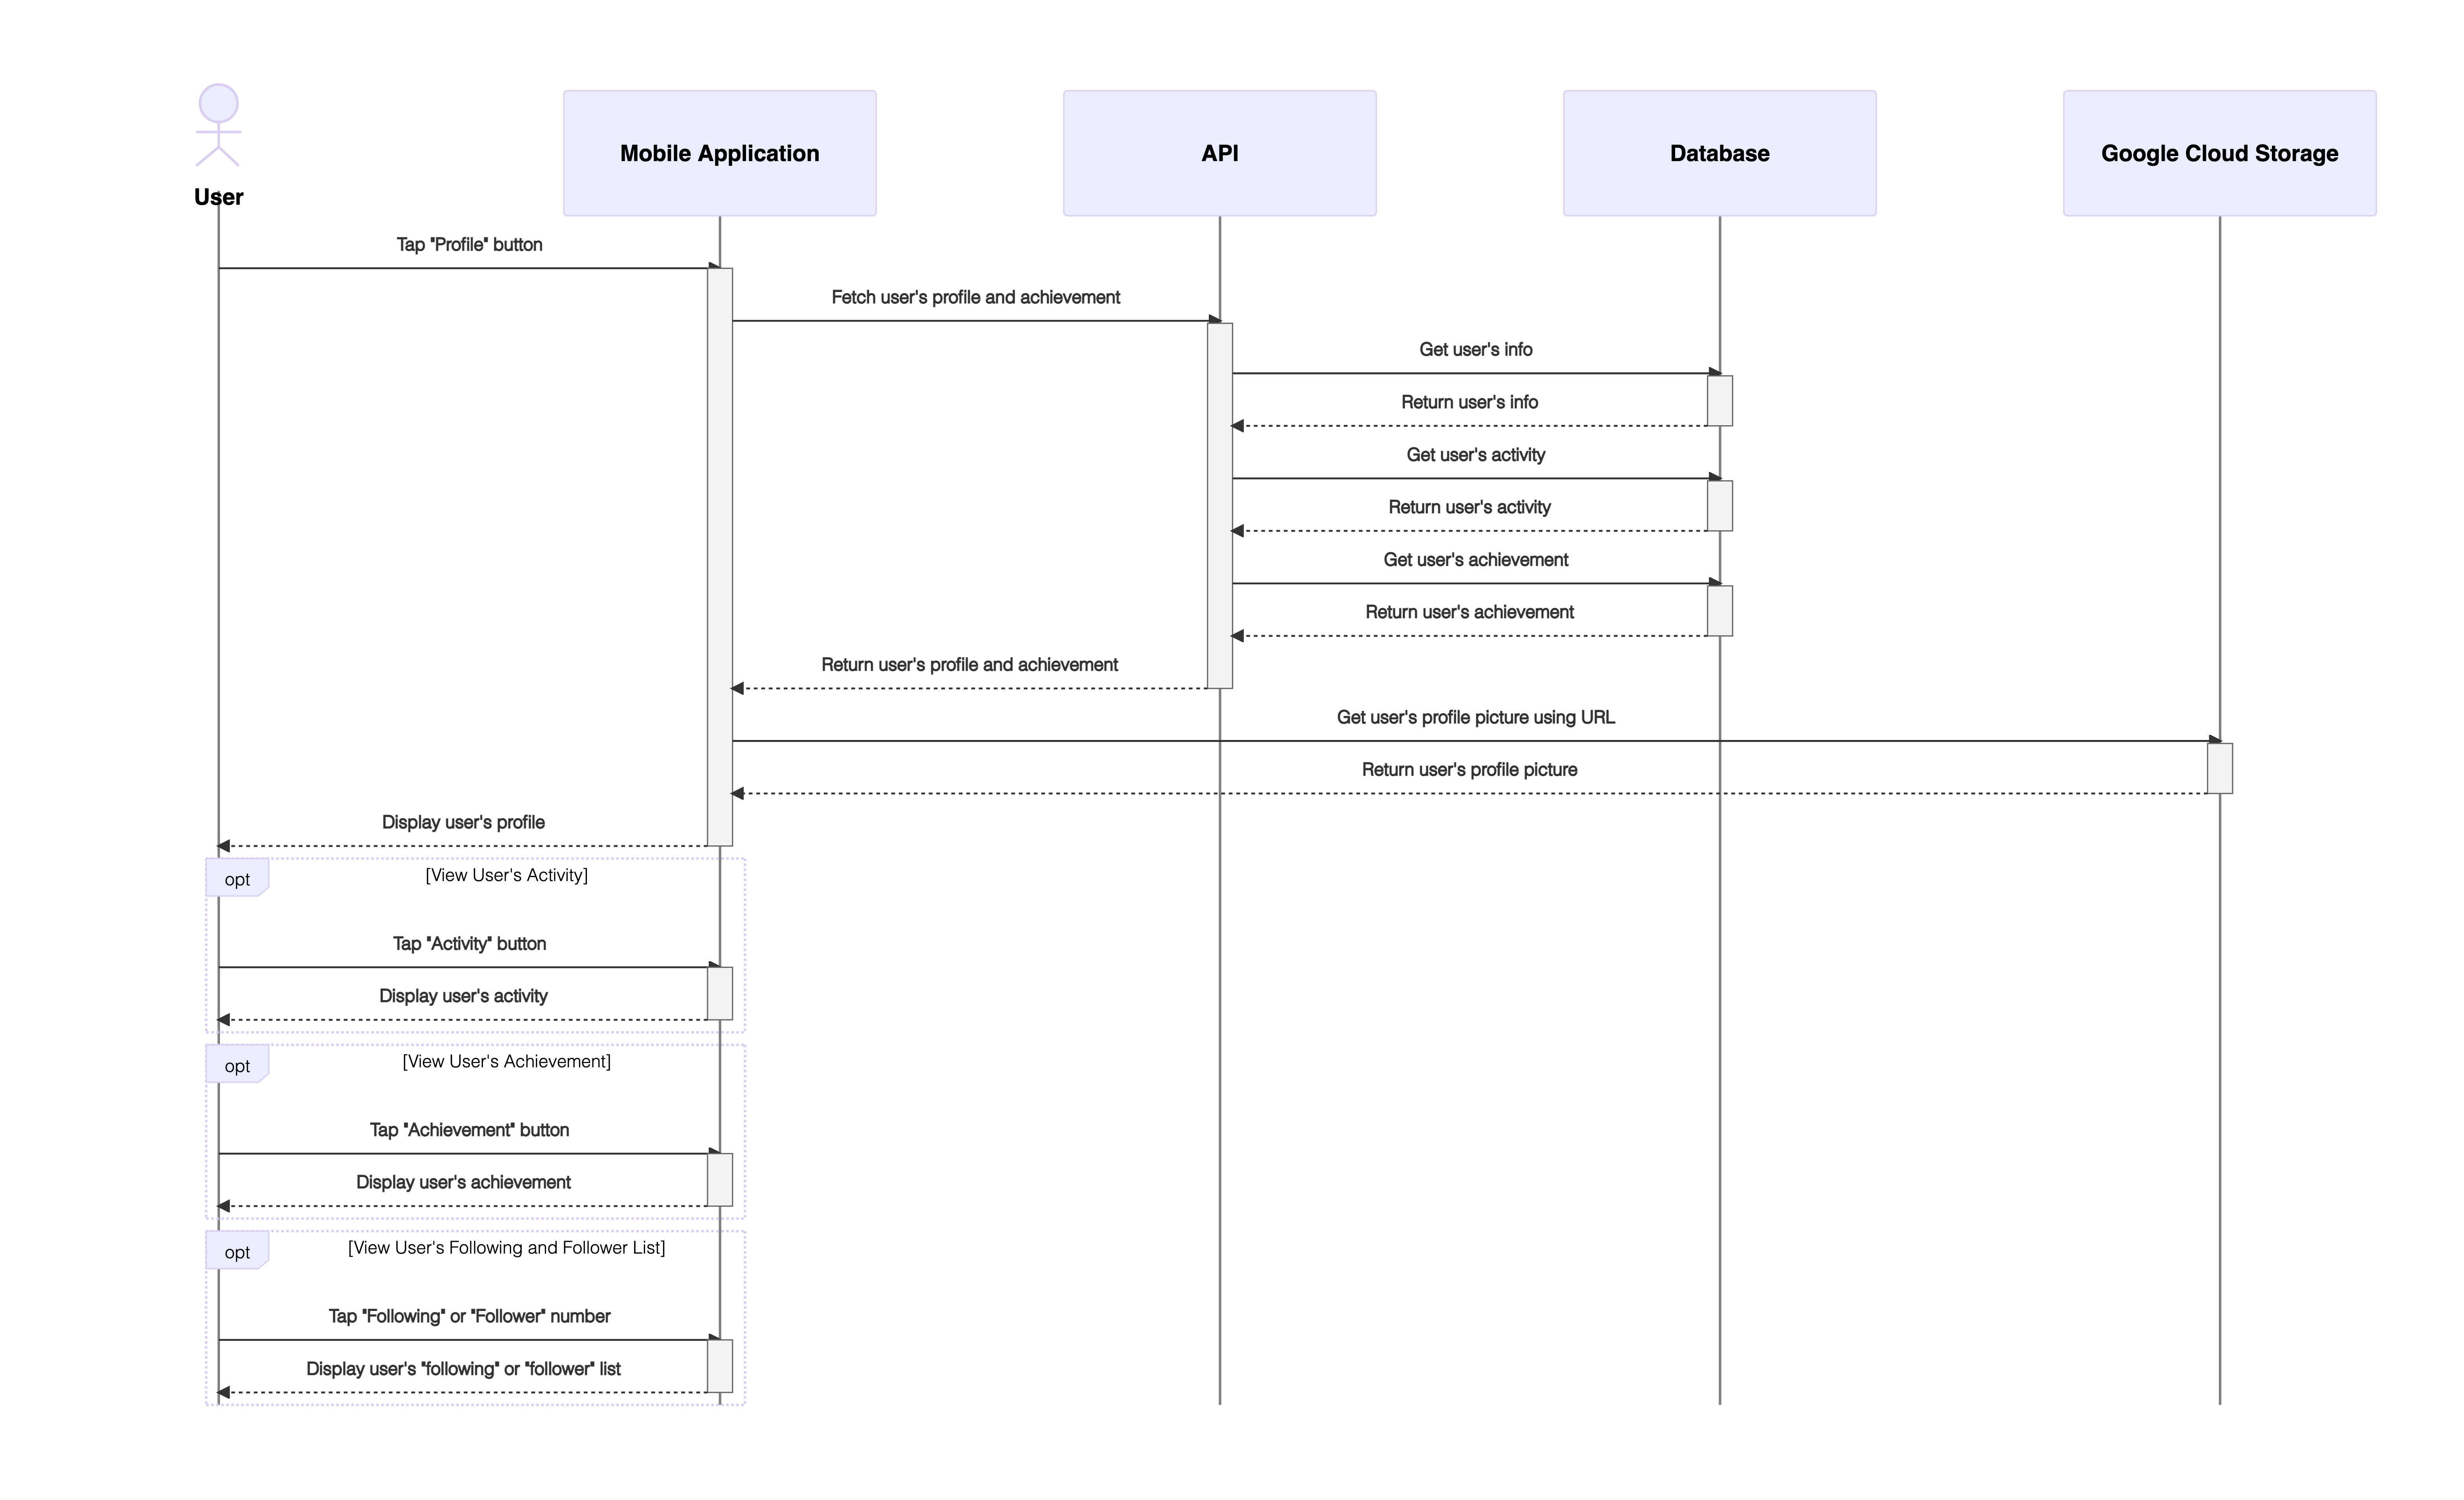
\includegraphics[width=\textwidth]{chapter_3/sequence/User Profile-1.md.png}
    \caption{การทำงานในส่วนข้อมูลของผู้ใช้}
\end{figure}

\begin{figure}
    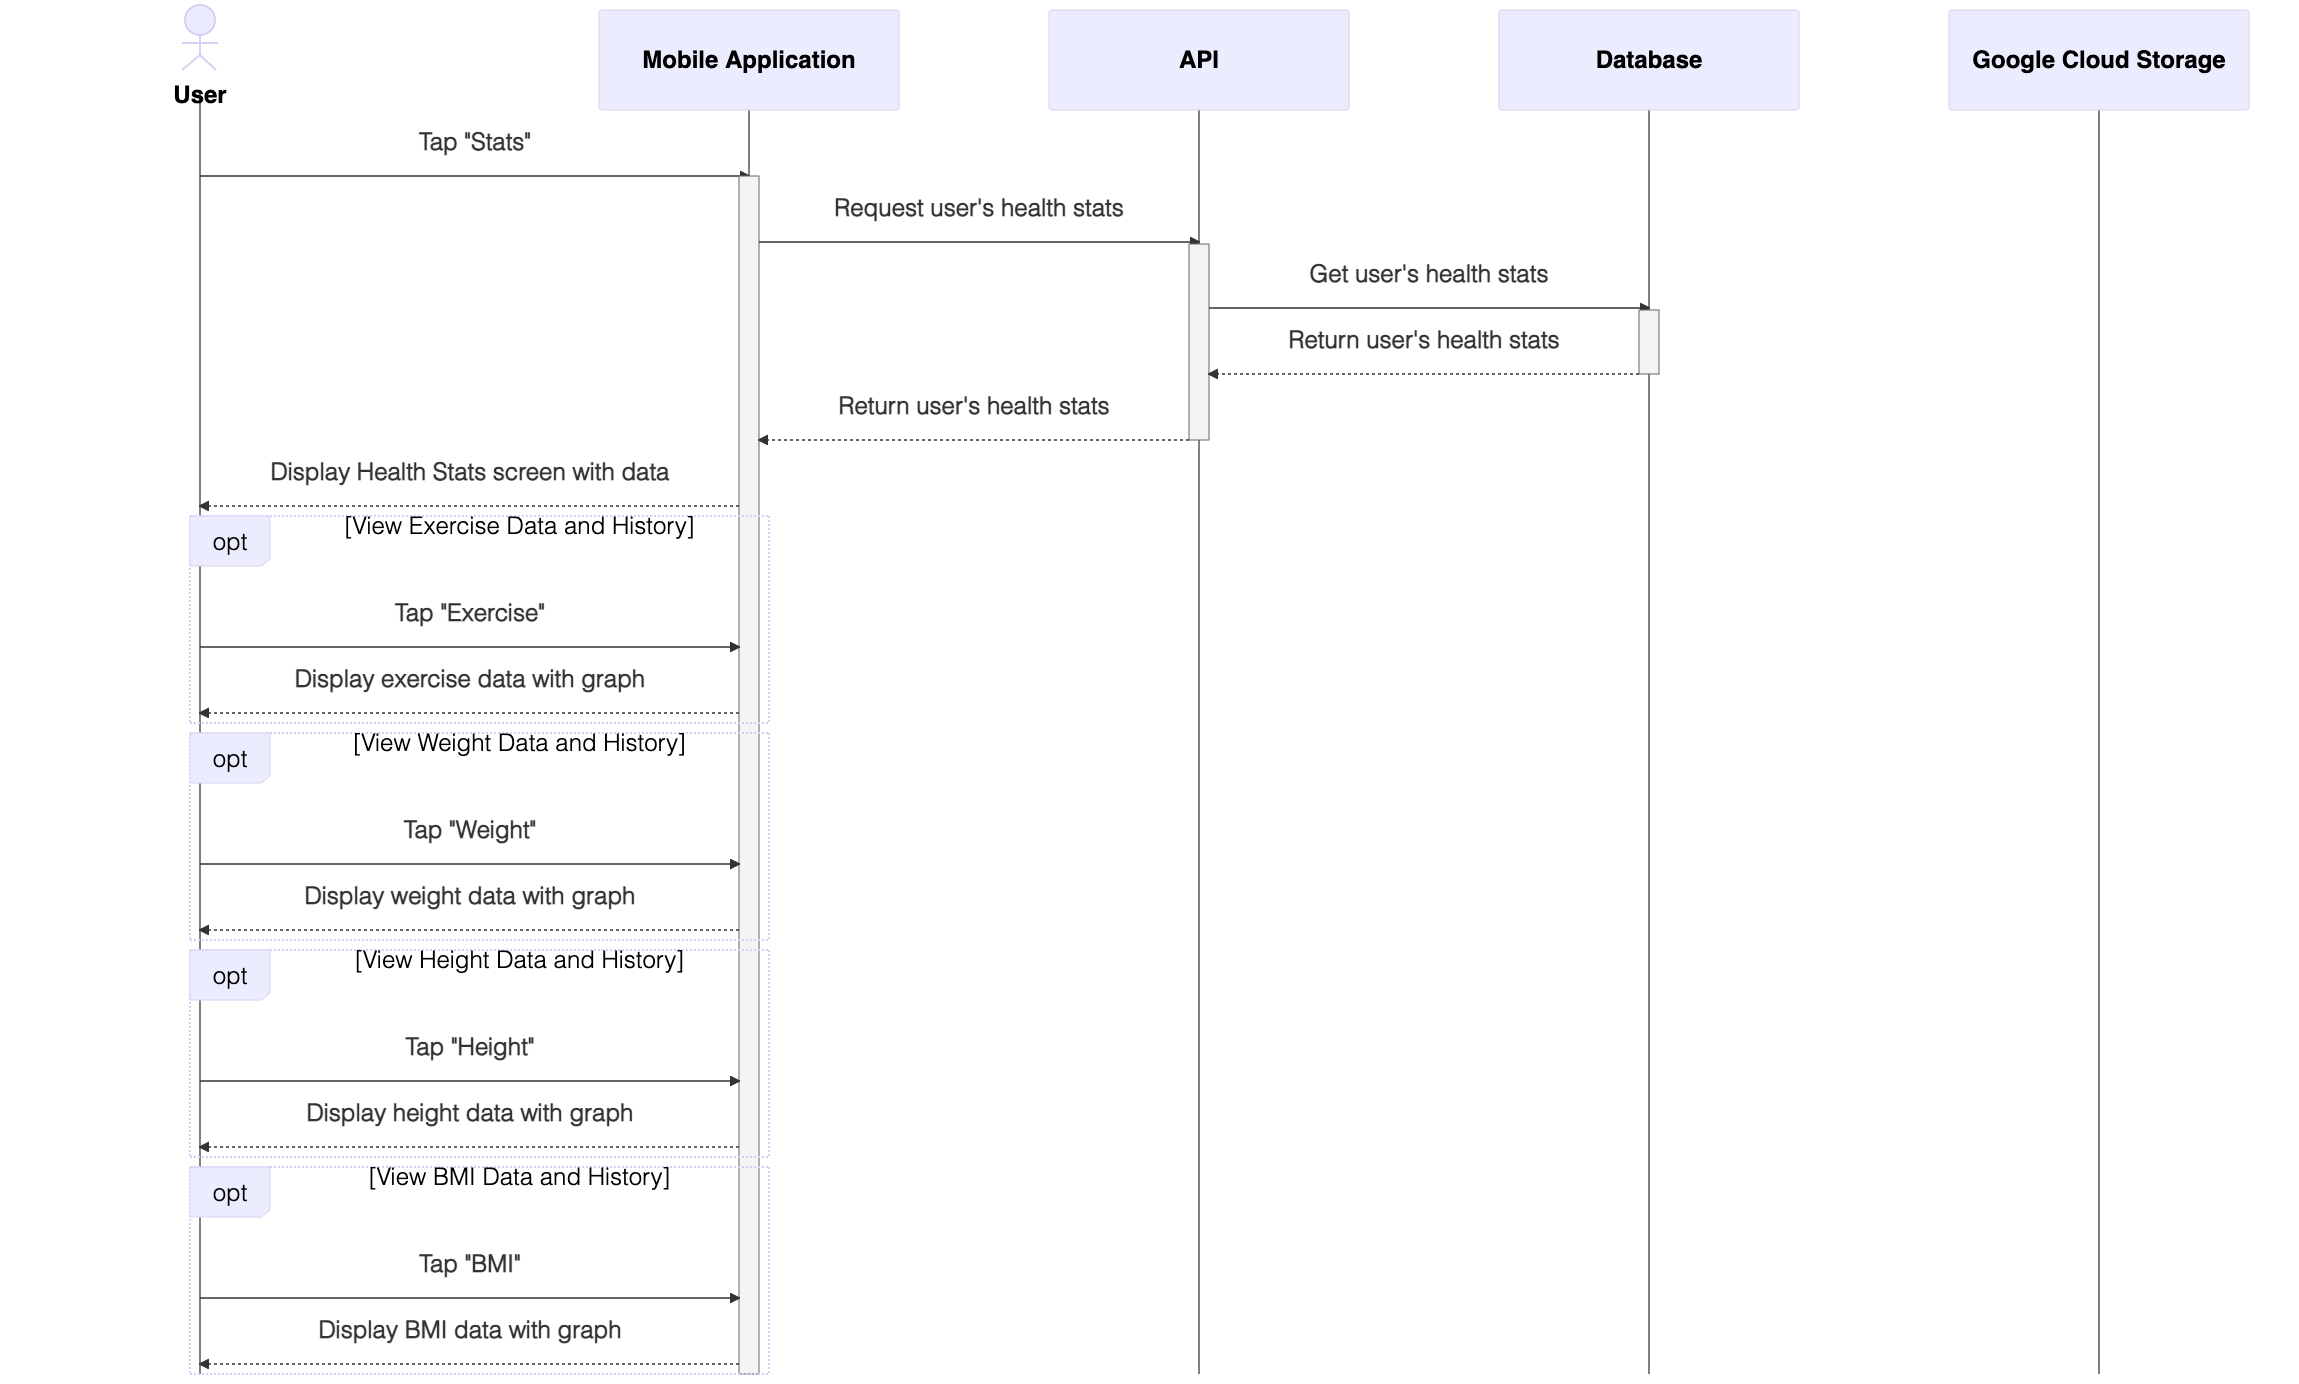
\includegraphics[width=\textwidth]{chapter_3/sequence/View Personal Health Stats-1.md.png}
    \caption{การทำงานในส่วนข้อมูลสุขภาพของผู้ใช้}
\end{figure}

\begin{figure}
    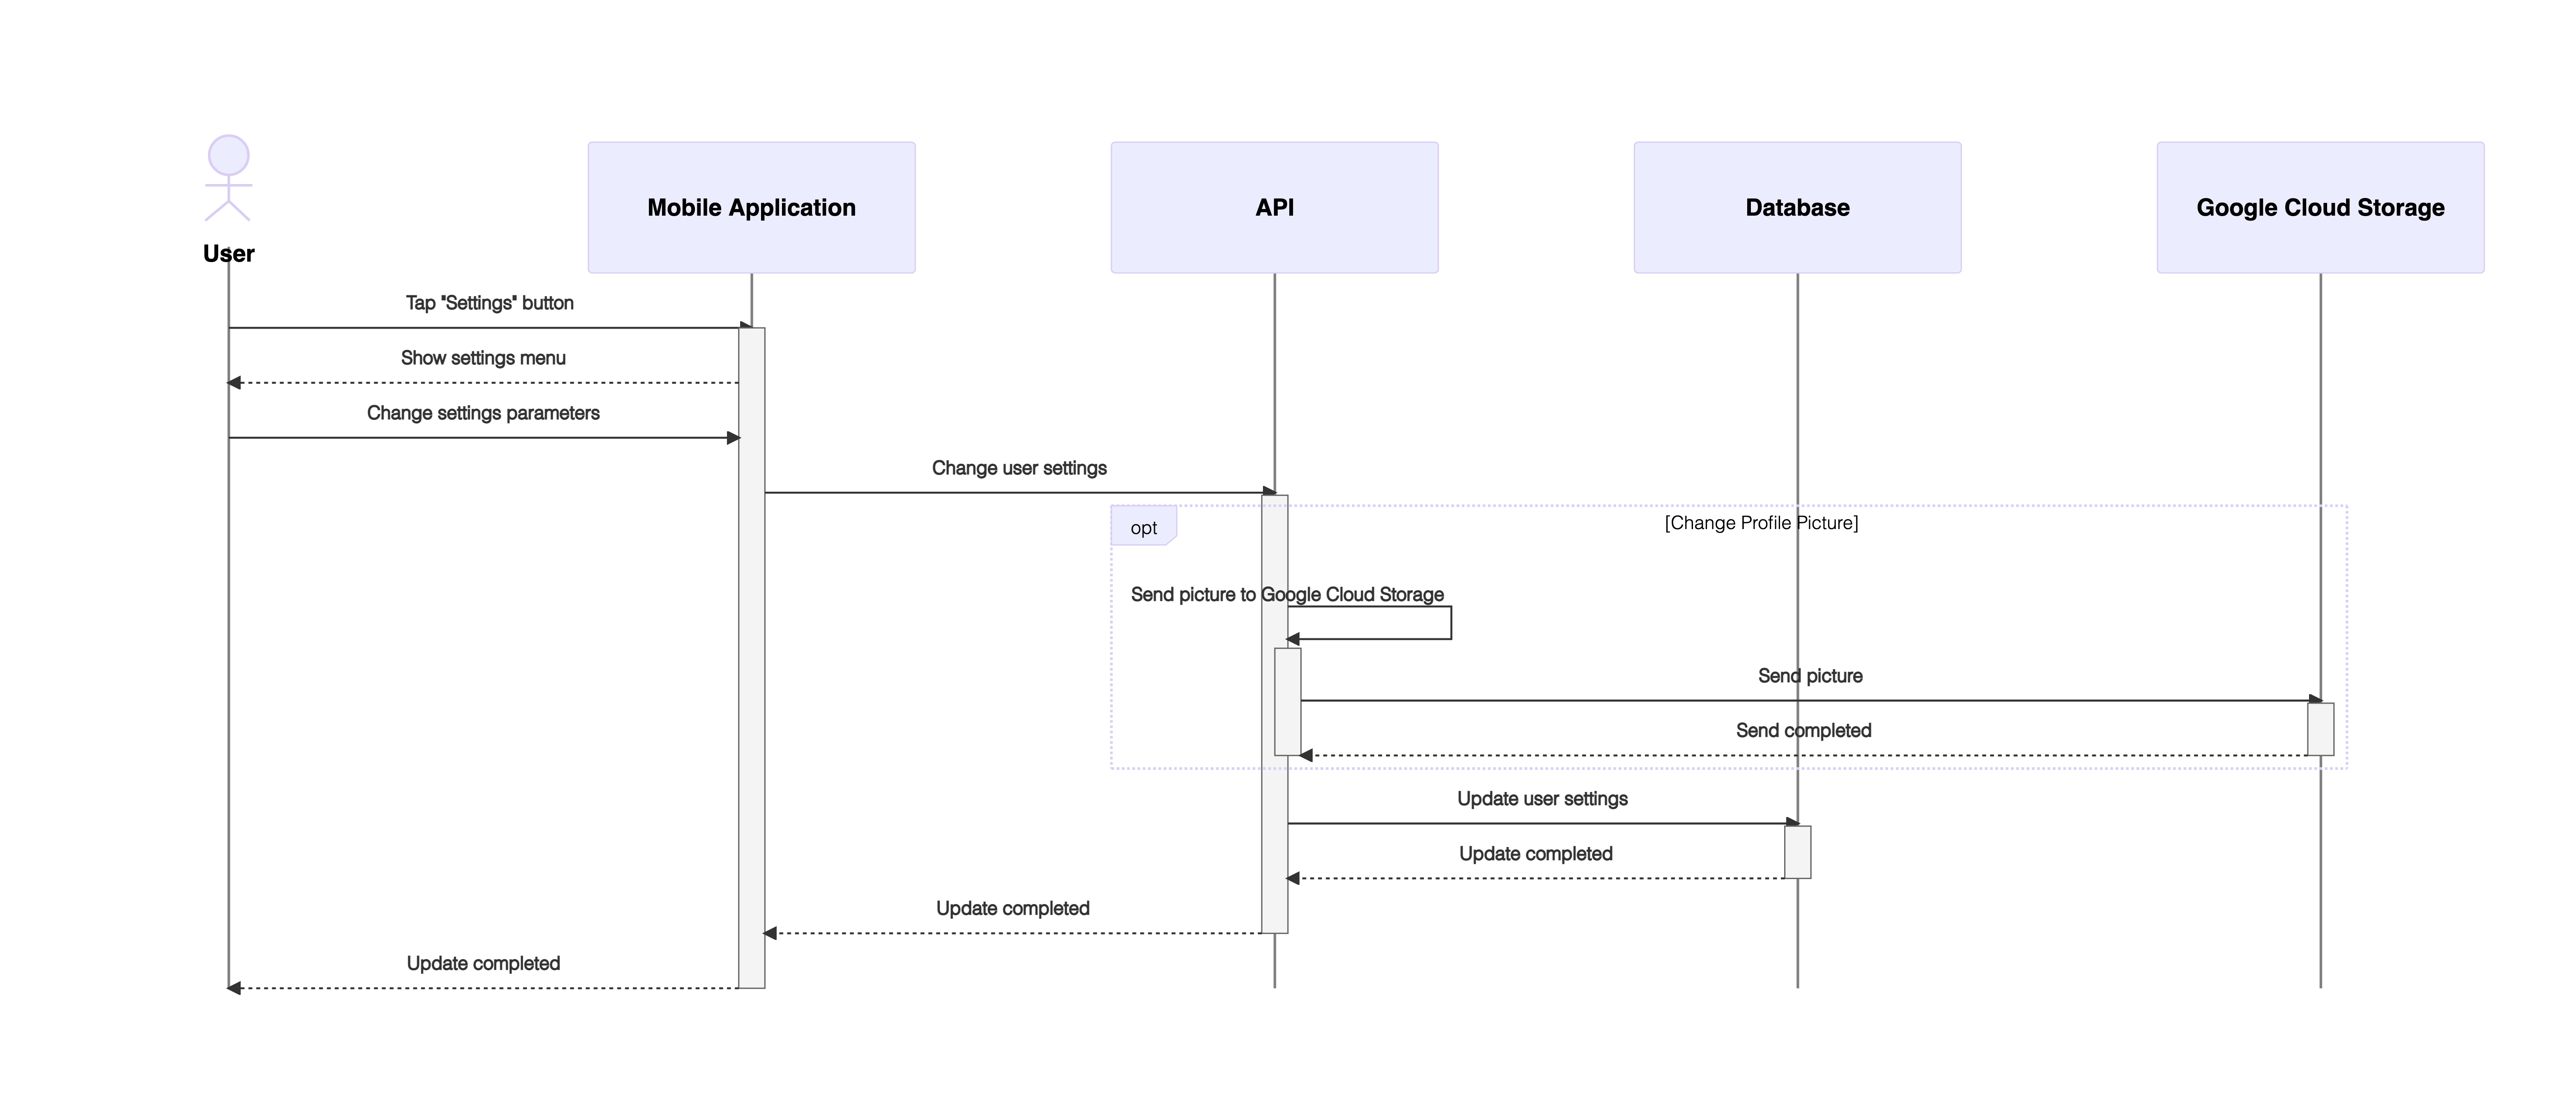
\includegraphics[width=\textwidth]{chapter_3/sequence/User Settings-1.md.png}
    \caption{การทำงานในส่วนการตั้งค่าบัญชีผู้ใช้}
\end{figure}

\clearpage

\section{การออกแบบส่วนติดต่อของผู้ใช้ (User Interface)}

การออกแบบส่วนติดต่อของผู้ใช้ในแอปพลิเคชัน มีดังนี้
\subsection{หน้าเข้าสู่ระบบ}
หน้าเข้าสู่ระบบ จะแสดงขึ้นเมื่อผู้ใช้เข้าสู่แอปพลิเคชัน ผู้ใช้จะต้องกรอก Email และ Password ที่ได้ลงทะเบียนไว้ จากนั้นจึงกด Sign In เพื่อเข้าสู่ระบบ
\begin{figure}
    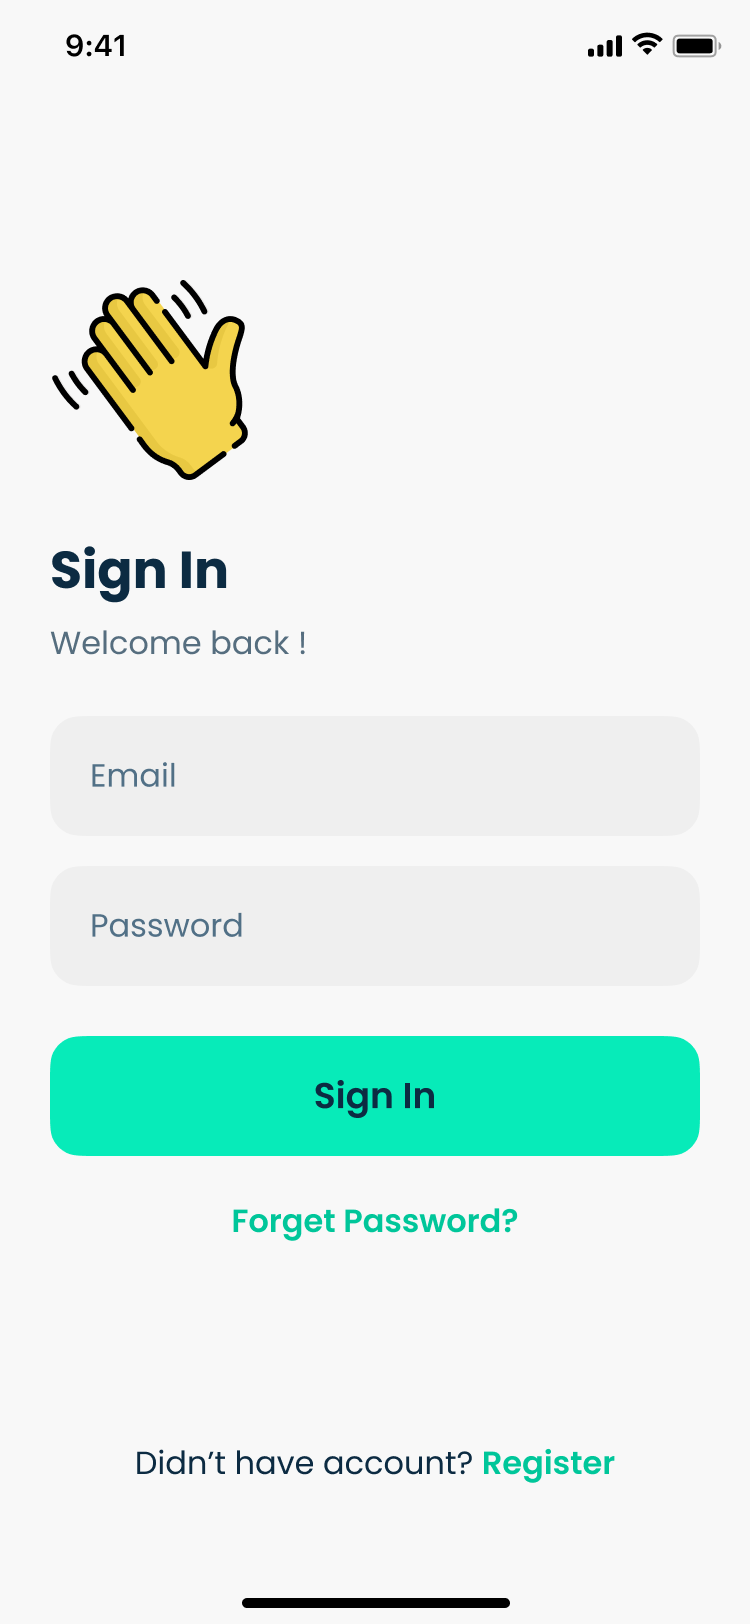
\includegraphics[height=10cm]{chapter_3/ui/Sign In.png}
    \caption{หน้าเข้าสู่ระบบ}
\end{figure}

\subsection{หน้าลงทะเบียน}
หน้าลงทะเบียน จะให้ผู้ใช้กรอกข้อมูลต่าง ๆ ดังนี้
\begin{enumerate}
    \item Email ที่จะใช้ลงทะเบียน
    \item Password ของบัญชี
\end{enumerate}
\begin{figure}
    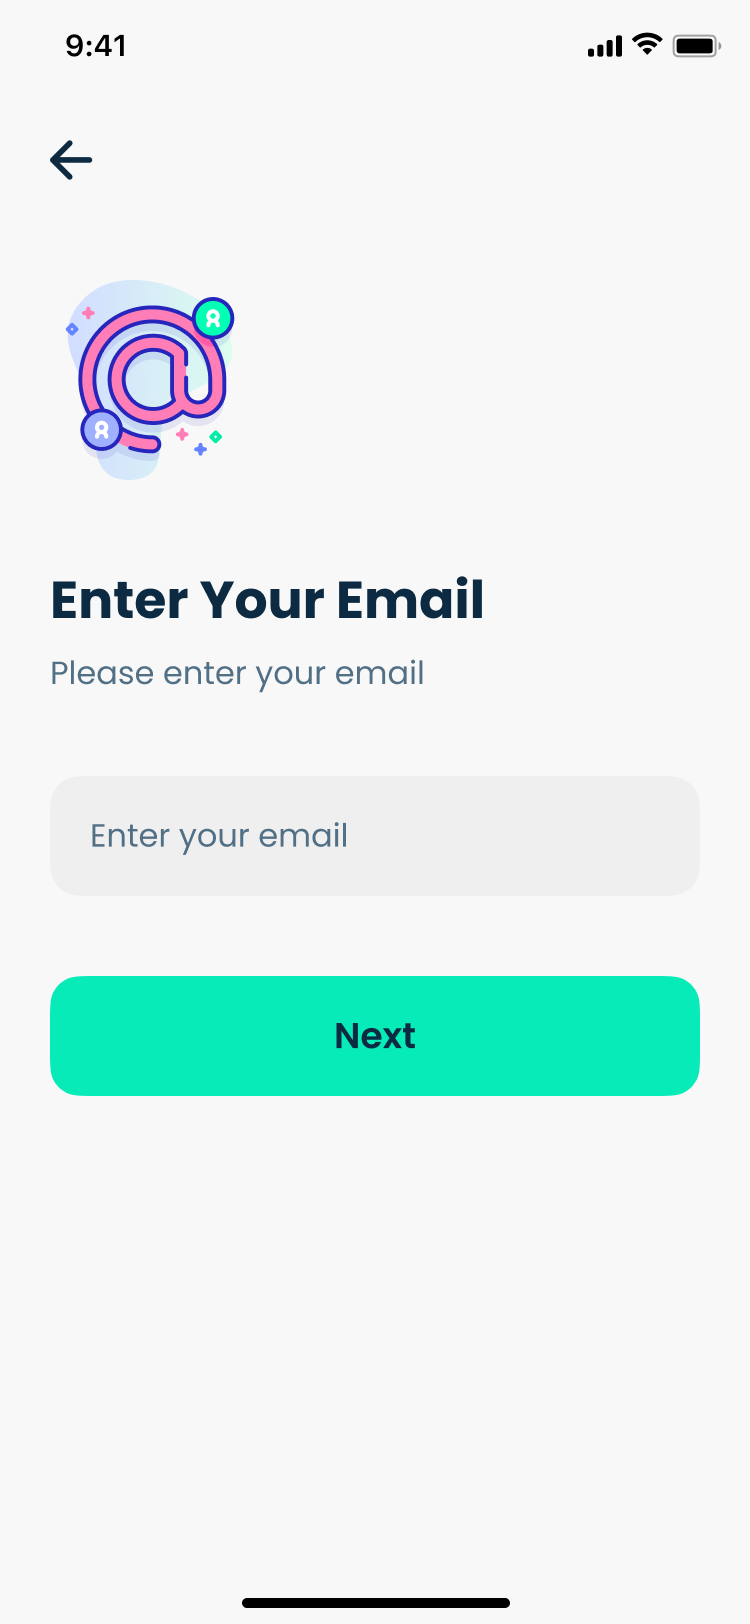
\includegraphics[height=10cm]{chapter_3/ui/Register/Email.png}
    \caption{หน้าการกรอก Email ที่จะใช้ลงทะเบียน}
\end{figure}
\begin{figure}
    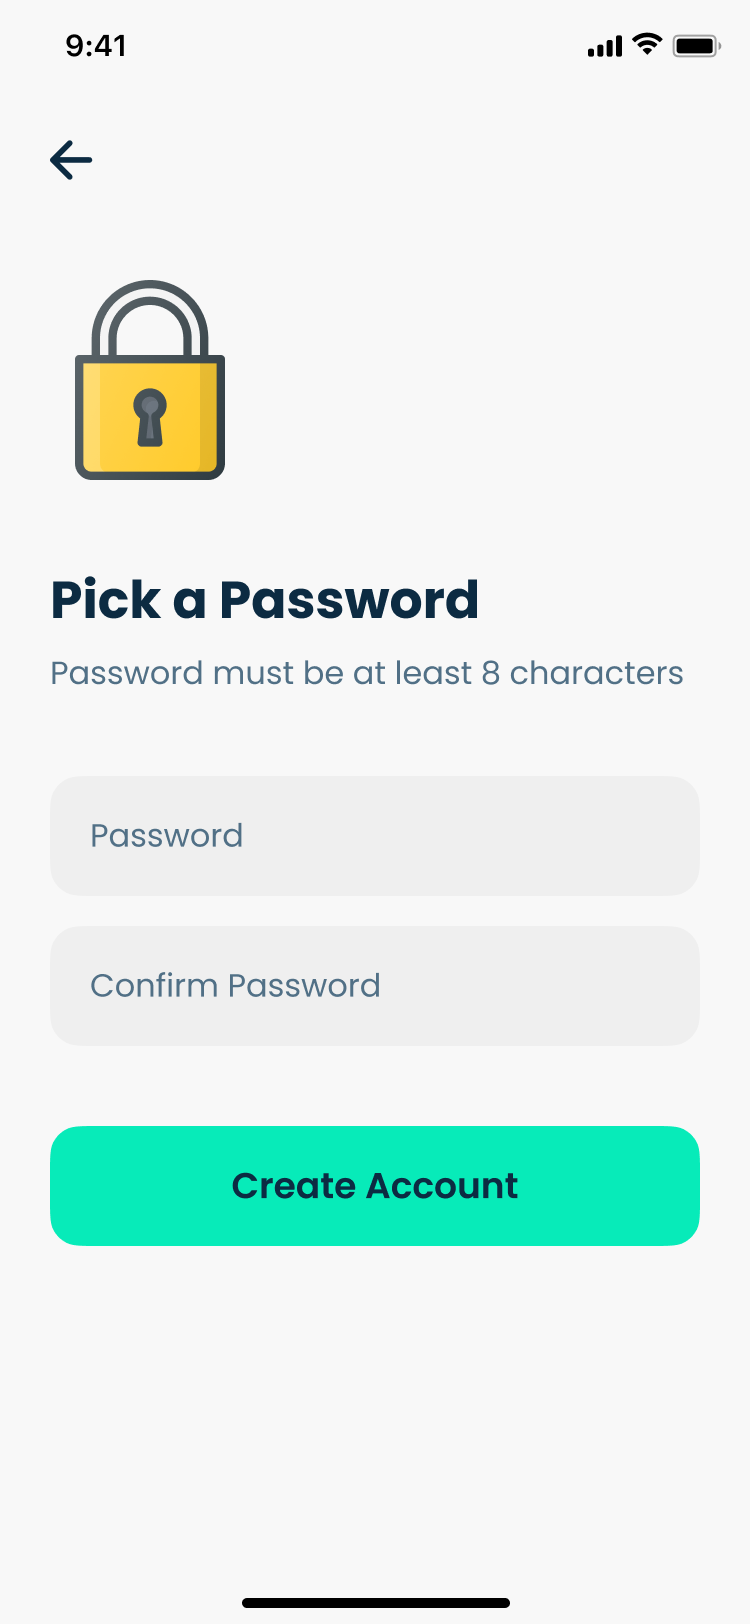
\includegraphics[height=10cm]{chapter_3/ui/Register/Password.png}
    \caption{หน้าการกำหนดรหัสผ่าน}
\end{figure}
\begin{figure}
    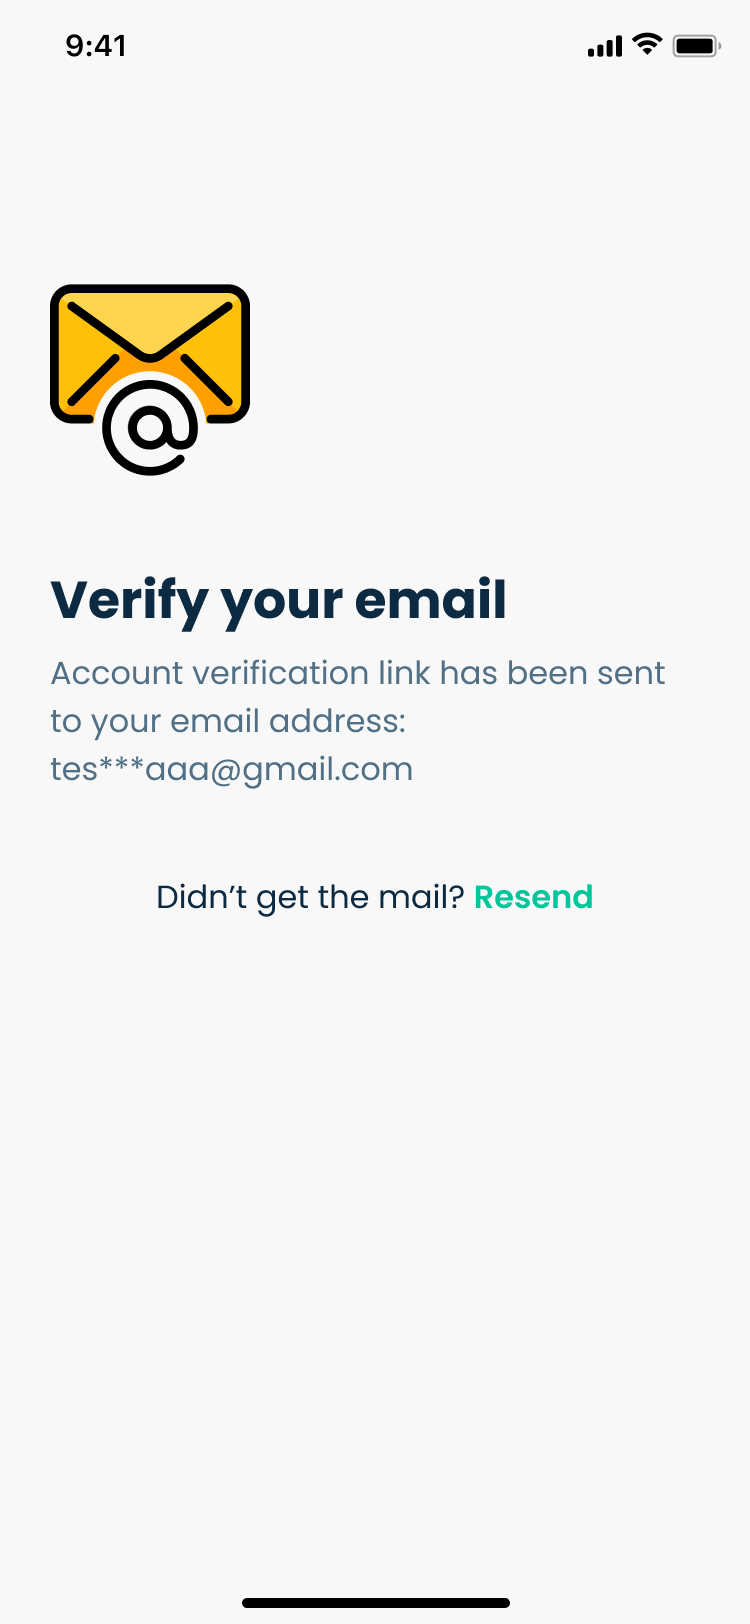
\includegraphics[height=10cm]{chapter_3/ui/Register/Email Verification.png}
    \caption{หน้าการ Verify อีเมล}
\end{figure}
\indent จากนั้น ระบบจะแจ้งให้ผู้ใช้ยืนยัน Email ที่ได้กรอกไว้ ซึ่งจะให้ผู้ใช้ตรวจสอบ Email ที่ระบบได้ส่งไป เมื่อผู้ใช้ยืนยันตัวตนเรียบร้อยแล้ว 
แอปพลิเคชันจะให้ผู้ใช้กรอกข้อมูล ดังนี้
\begin{enumerate}
    \item Display Name สำหรับบัญชีผู้ใช้ ซึ่งจะใช้ในการให้ผู้อื่นสามารถค้นหาบัญชีได้
    \item Profile Picture ให้ผู้ใช้อัปโหลดรูปโปรไฟล์ของตัวเอง ซึ่งผู้ใช้สามารถข้ามขั้นตอนนี้ได้
\end{enumerate}
\begin{figure}
    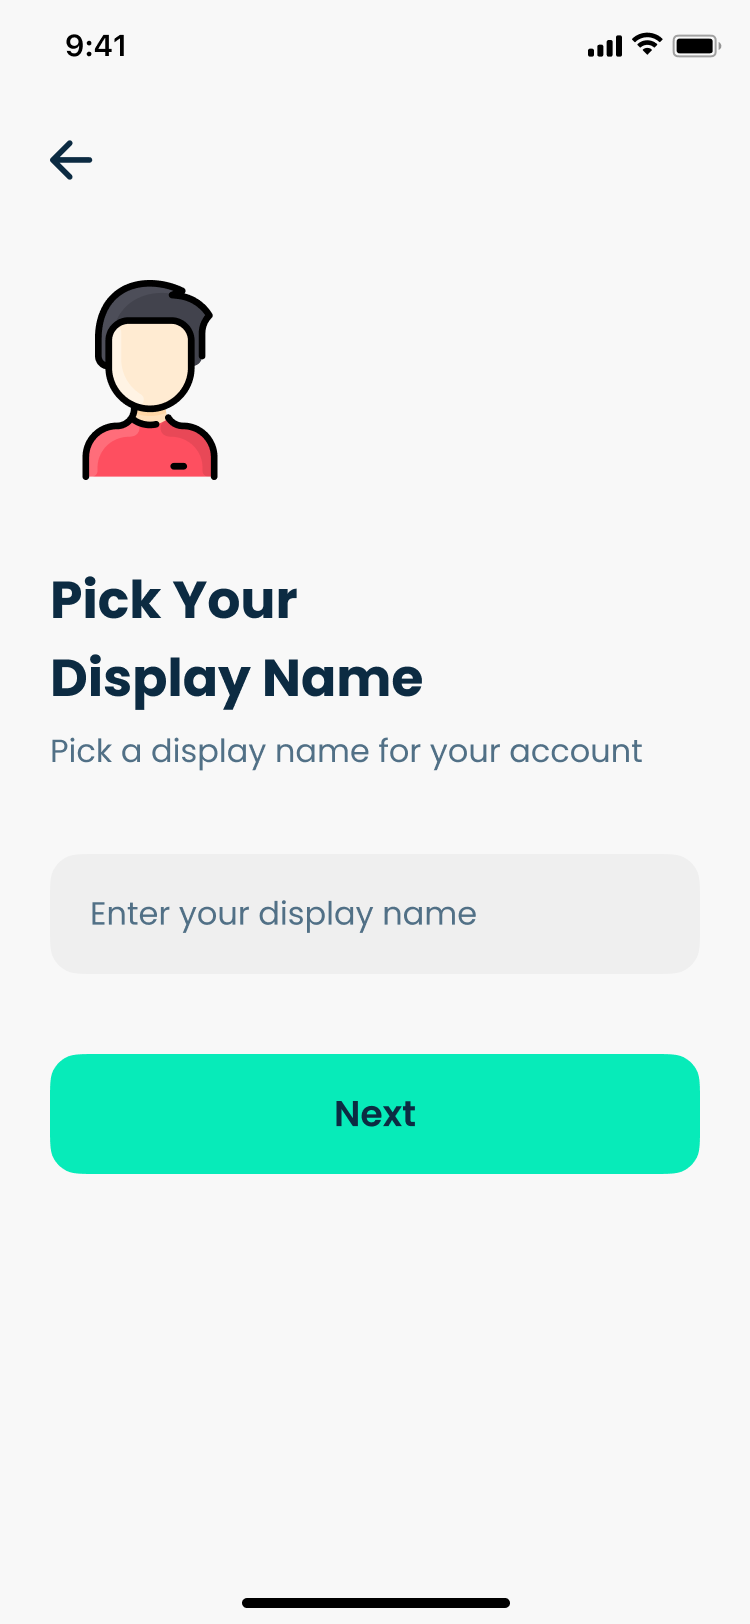
\includegraphics[height=10cm]{chapter_3/ui/Register/Display Name.png}
    \caption{หน้าการกรอก Display Name}
\end{figure}
\begin{figure}
    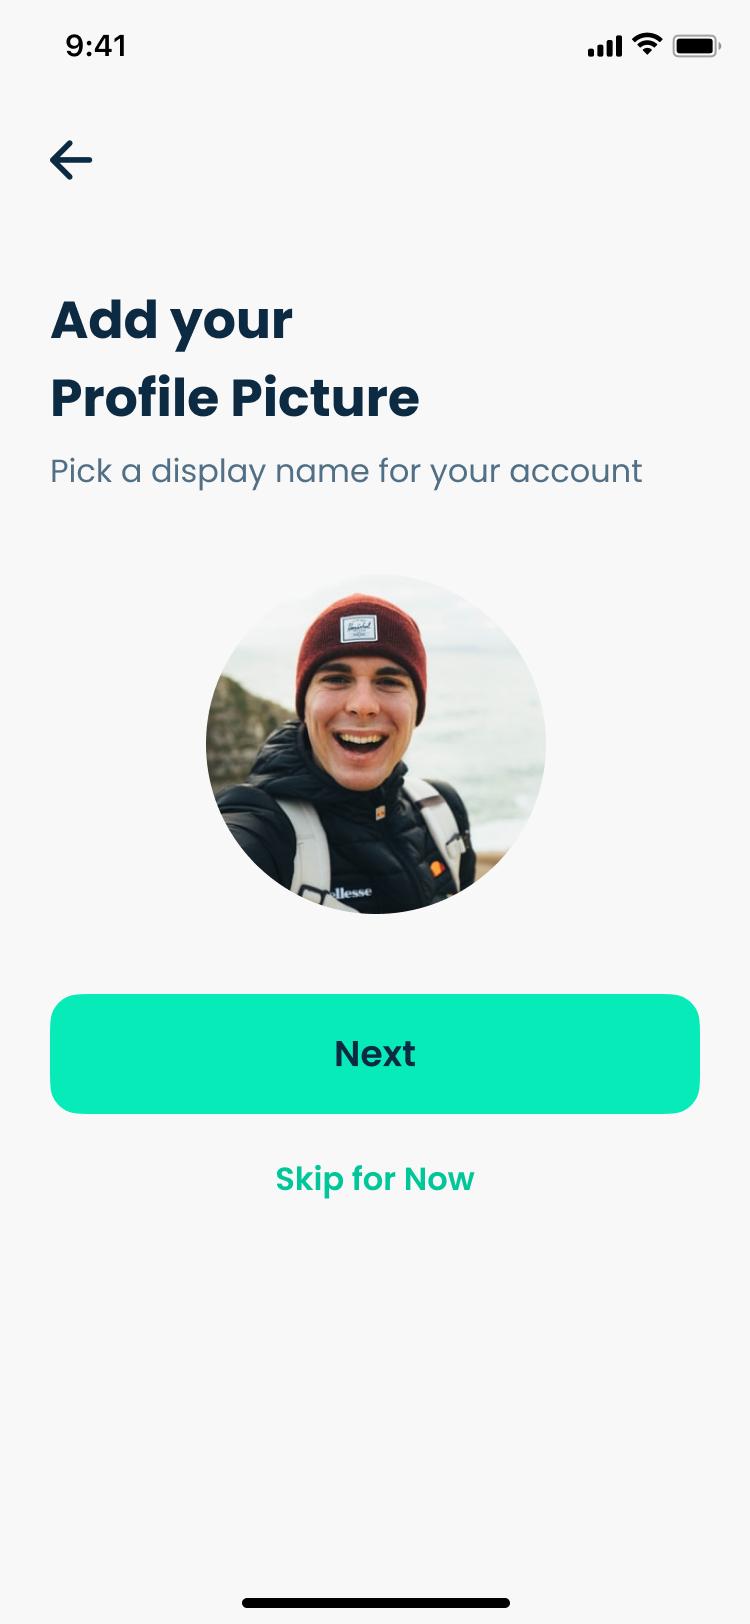
\includegraphics[height=10cm]{chapter_3/ui/Register/Profile Picture.png}
    \caption{หน้าการเพิ่มรูปภาพของผู้ใช้}
\end{figure}

\subsection{หน้าหลังจากการลงทะเบียน}
เมื่อผู้ใช้ลงทะเบียนเรียบร้อยแล้ว ระบบจะถามคำถามต่าง ๆ เพื่อให้ระบบทราบถึงความต้องการในการออกกำลังกาย และสามารถแนะนำคอร์สออกกำลังกายได้แม่นยำมากขึ้น ซึ่งระบบจะถามคำถาม ดังนี้
\begin{enumerate}
    \item เพศของผู้ใช้
    \item ปีเกิดของผู้ใช้
    \item น้ำหนักและส่วนสูงของผู้ใช้
    \item ประเภทของการออกกำลังกายที่ชื่นชอบ
    \item ส่วนของร่างกายที่ต้องการหลีกเลี่ยง
\end{enumerate}

\begin{figure}
    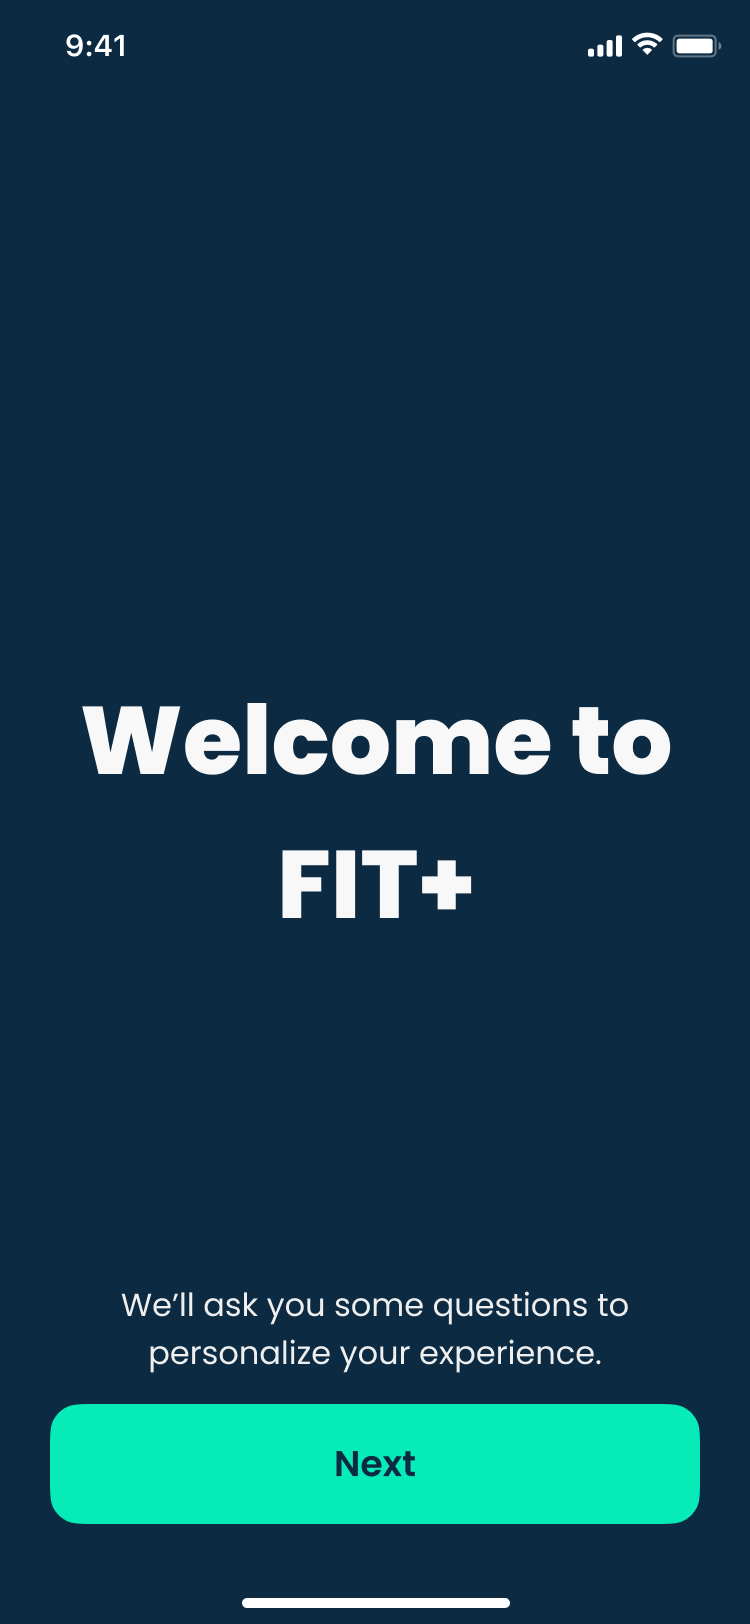
\includegraphics[height=10cm]{chapter_3/ui/New User Setup/000 - Welcome.png}
    \caption{หน้าหลังจากการยืนยันตัวตนเรียบร้อยแล้ว}
\end{figure}
\begin{figure}
    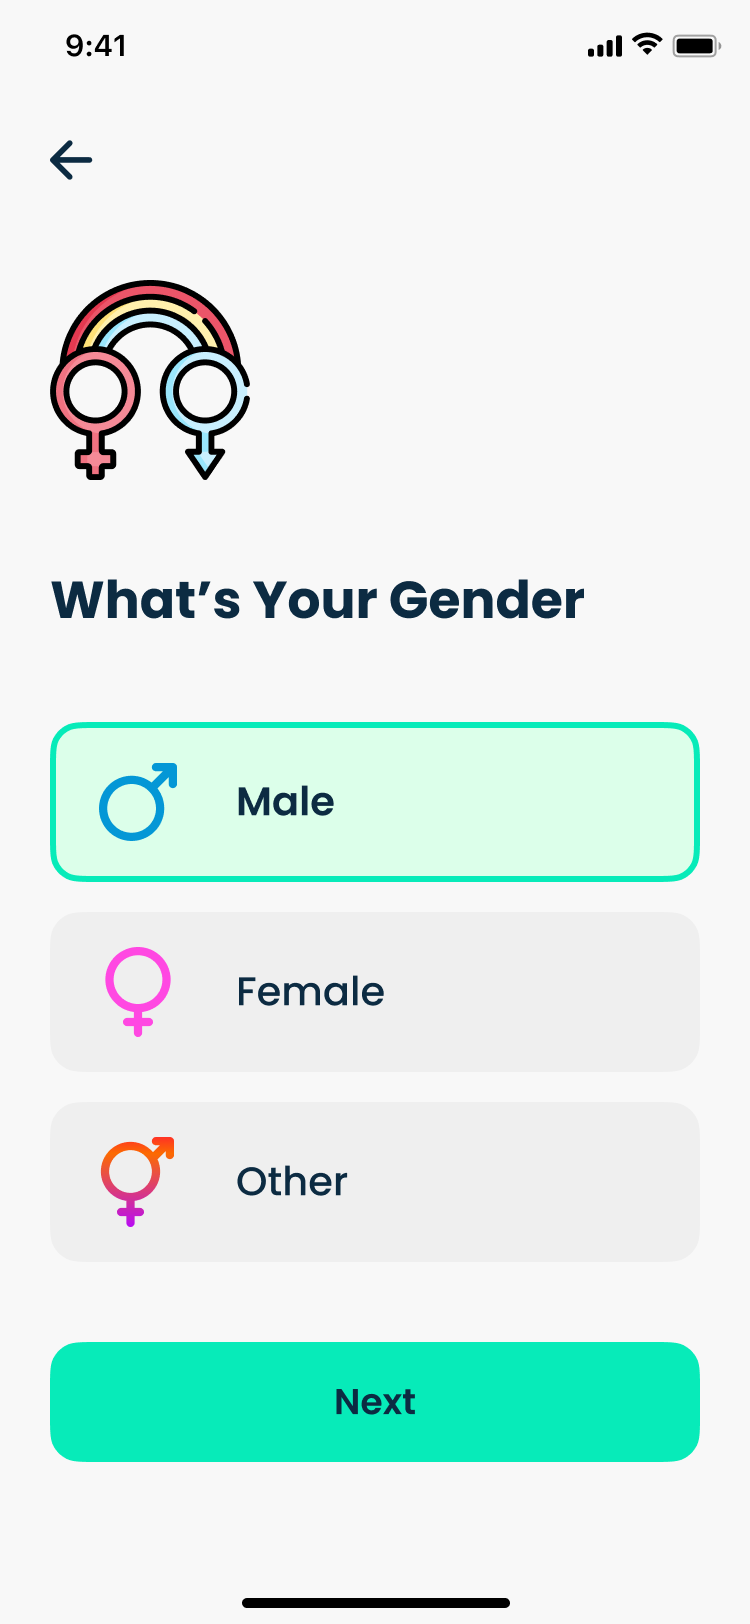
\includegraphics[height=10cm]{chapter_3/ui/New User Setup/001 - Gender.png}
    \caption{หน้าการระบุเพศ}
\end{figure}
\begin{figure}
    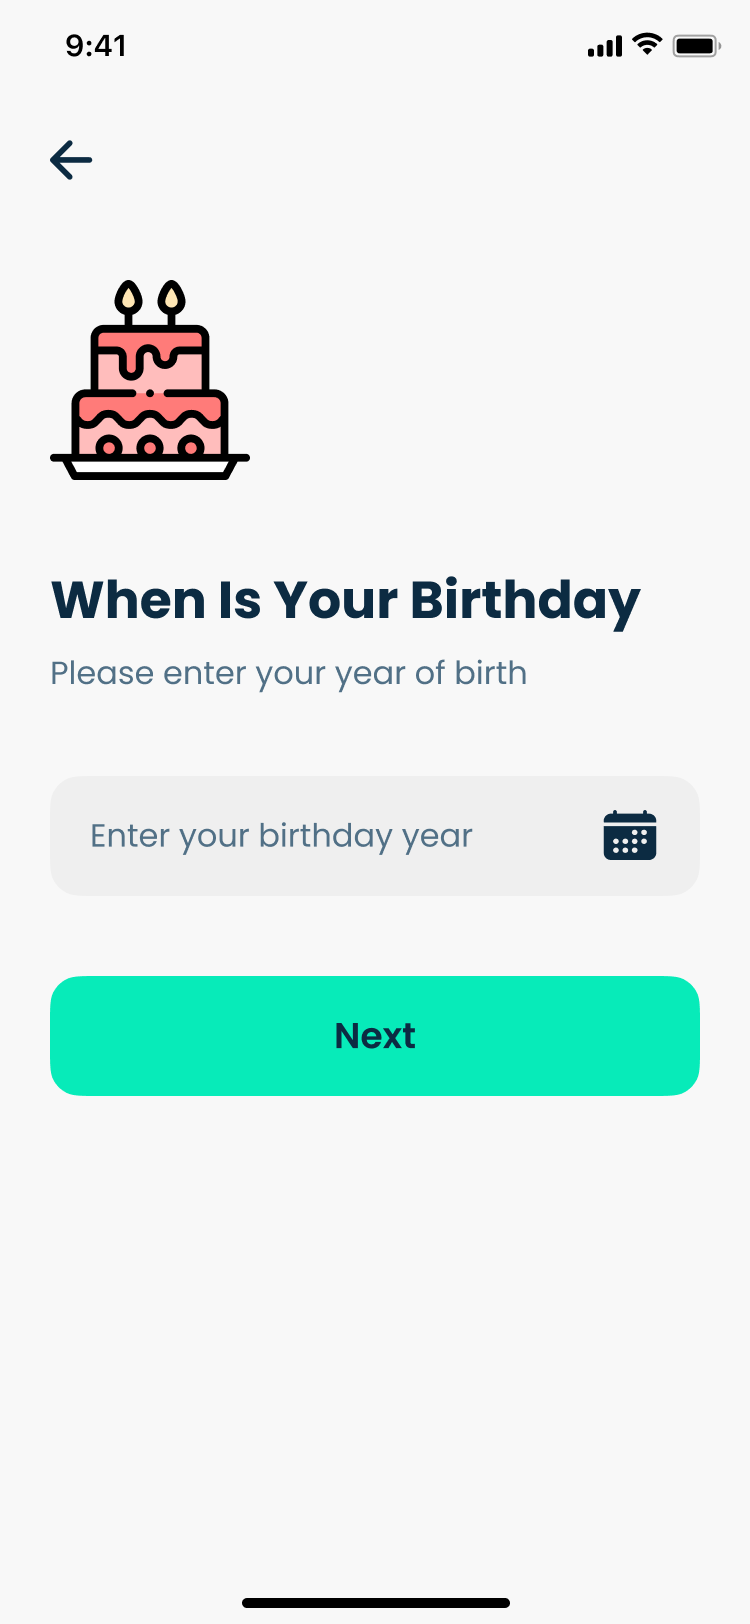
\includegraphics[height=10cm]{chapter_3/ui/New User Setup/002 - Birthday.png}
    \caption{หน้าการกรอกข้อมูลวันเกิด}
\end{figure}
\begin{figure}
    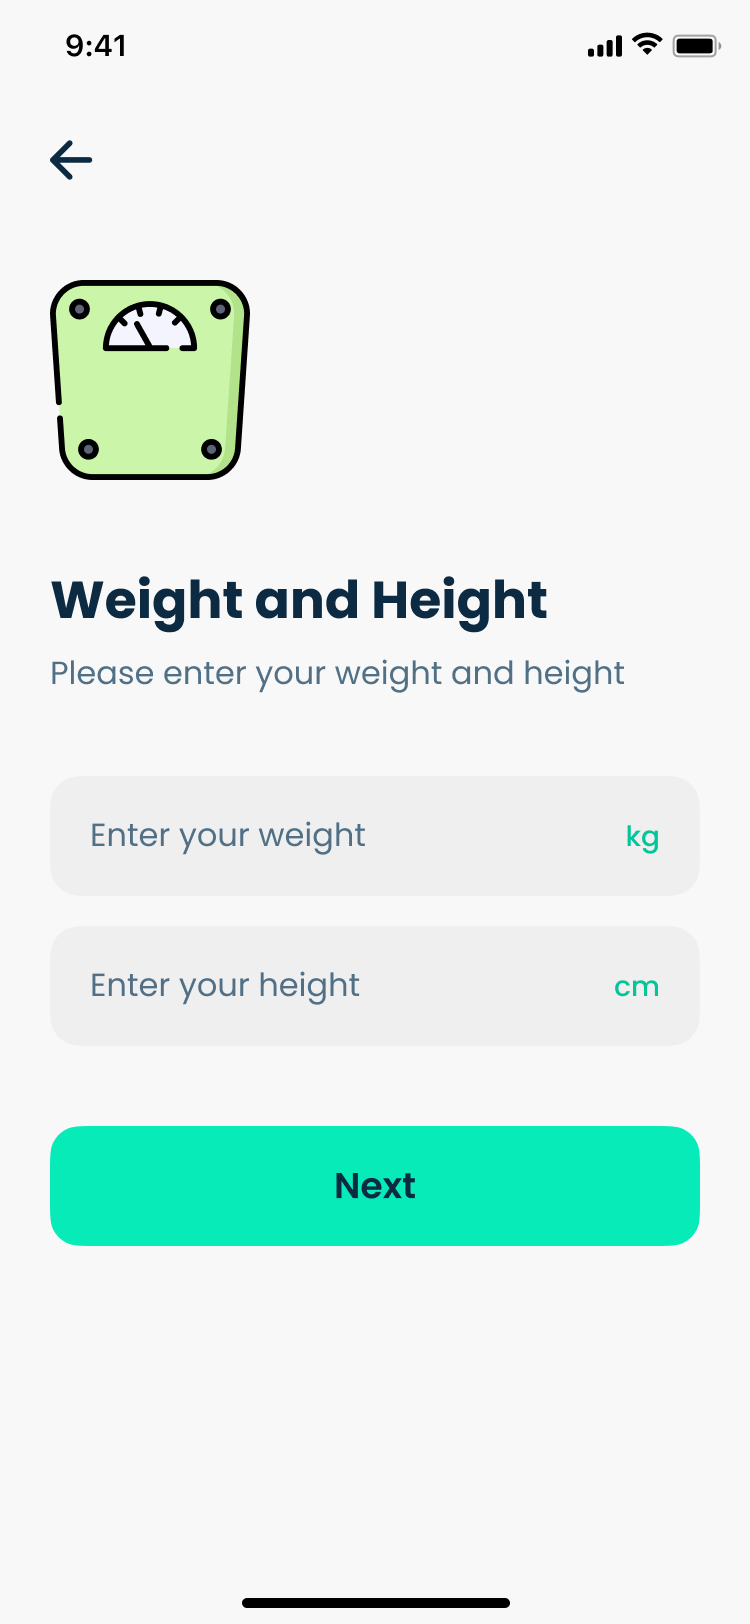
\includegraphics[height=10cm]{chapter_3/ui/New User Setup/003 - Weight and Height.png}
    \caption{หน้าการกรอกข้อมูลน้ำหนักและส่วนสูง}
\end{figure}
\begin{figure}
    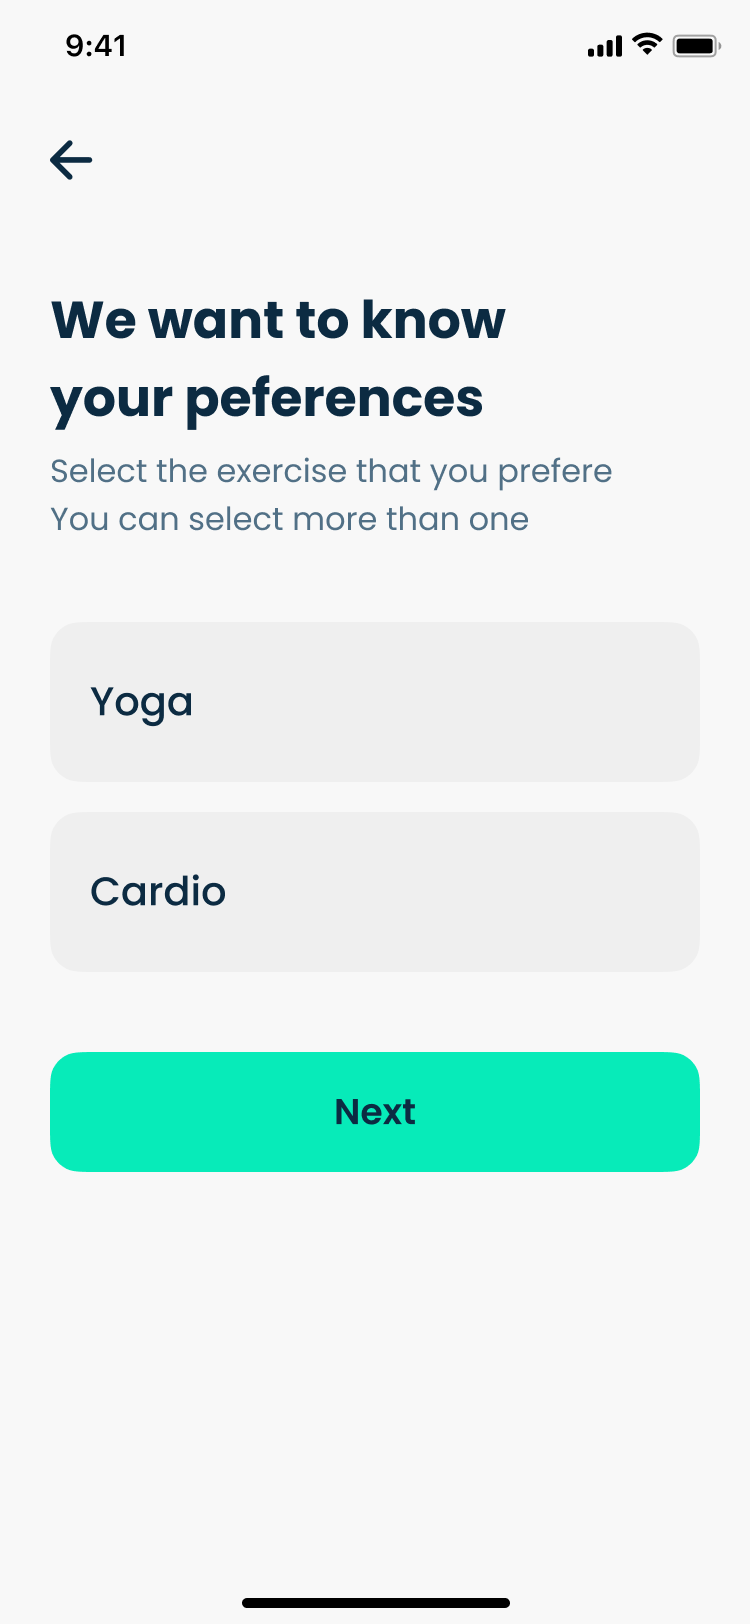
\includegraphics[height=10cm]{chapter_3/ui/New User Setup/004 - Exercise Preferences.png}
    \caption{หน้าการระบุประเภทของการออกกำลังกายที่ชื่นชอบ}
\end{figure}
\begin{figure}
    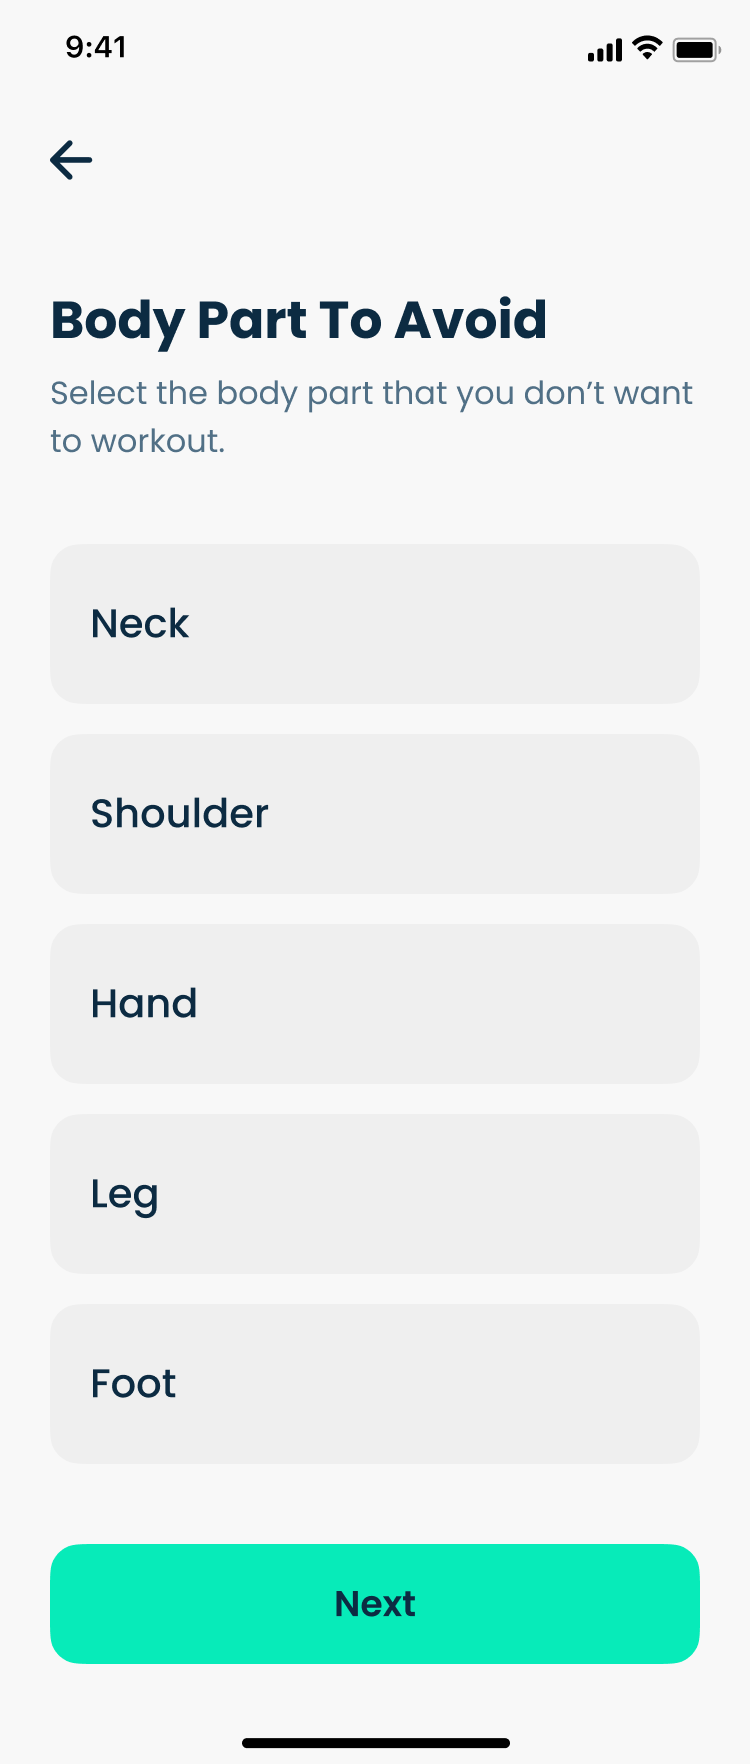
\includegraphics[height=10cm]{chapter_3/ui/New User Setup/005 - Exercise Preferences.png}
    \caption{หน้าการระบุส่วนของร่างกายที่ต้องการหลีกเลี่ยง}
\end{figure}
\begin{figure}
    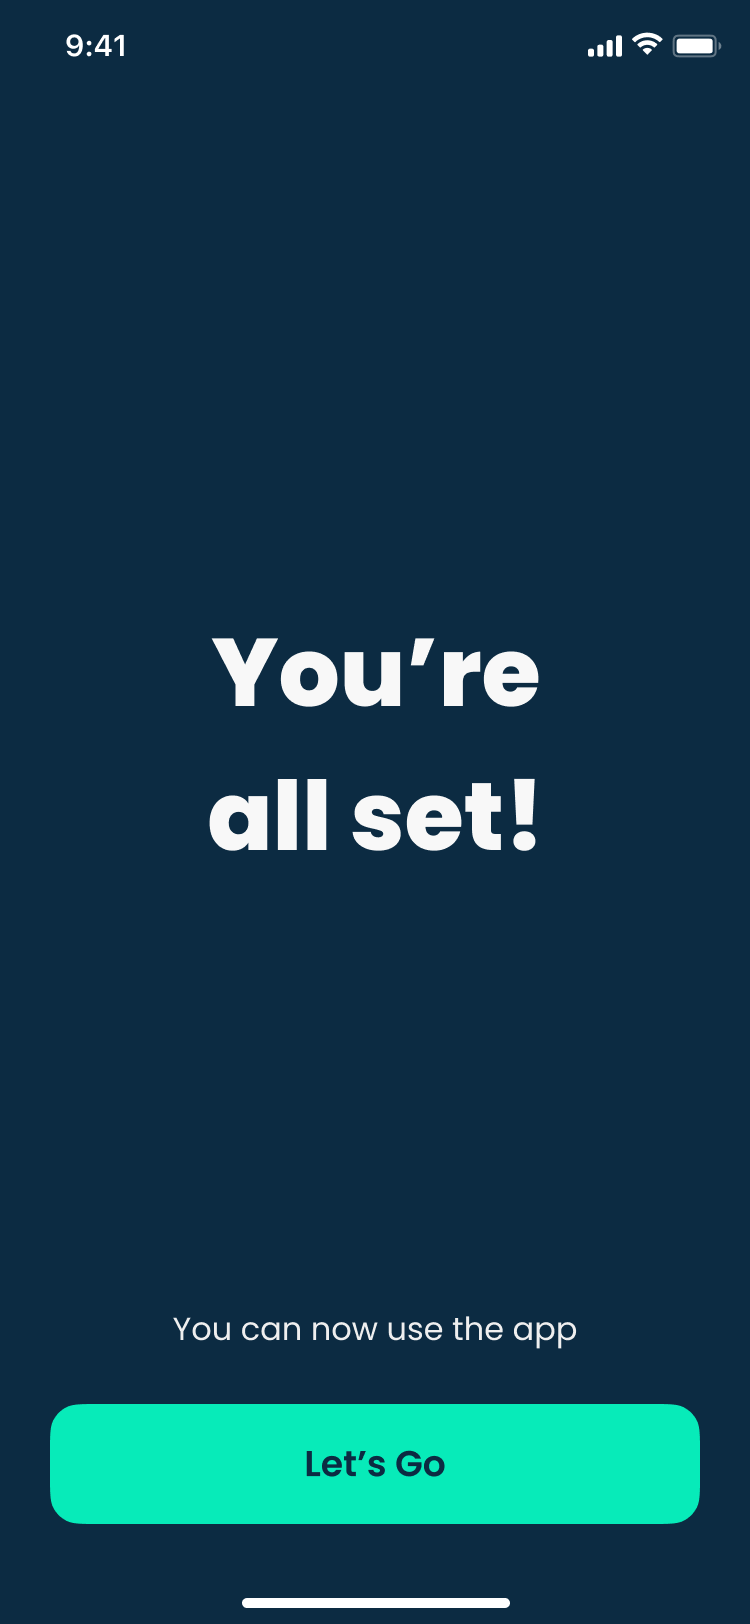
\includegraphics[height=10cm]{chapter_3/ui/New User Setup/006 - Complete.png}
    \caption{หน้าหลังจากการตอบคำถามความต้องการออกกำลังกาย}
\end{figure}

\subsection{หน้าแรกของแอปพลิเคชัน}
หน้าแรกของแอปพลิเคชัน จะแสดงผลคอร์สต่าง ๆ ที่เป็นที่นิยม และเหมาะสมสำหรับผู้ใช้ และแถบ Banner สำหรับการประชาสัมพันธ์คอร์สหรือข่าวสารต่าง ๆ ของทางแอปพลิเคชัน และด้านมุมบนขวาจะมีปุ่มค้นหา โดยจะสามารถค้นหาคอร์ส และบัญชีผู้ใช้ในระบบได้
\begin{figure}
    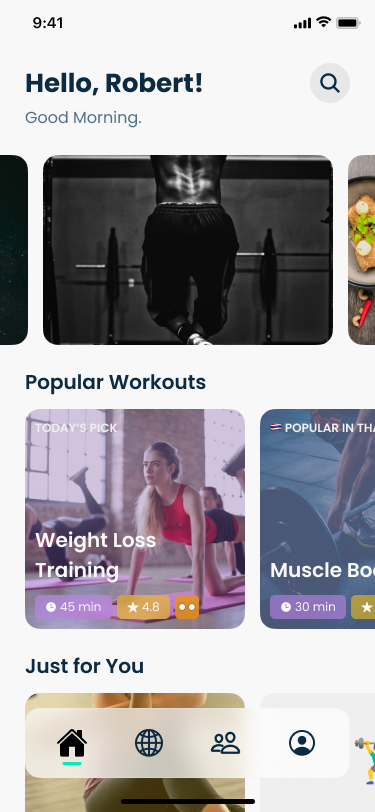
\includegraphics[height=10cm]{chapter_3/ui/Home.png}
    \caption{หน้าแรกของแอปพลิเคชัน}
\end{figure}

\subsection{หน้ากิจกรรมของผู้ใช้}
หน้ากิจกรรมของผู้ใช้ จะแสดงความเคลื่อนไหวต่าง ๆ ของบุคคลที่ผู้ใช้ได้ติดตามไว้ ผู้ใช้สามารถกด Reaction และ Comment กิจกรรมของบุคคลนั้น ๆ ได้ ด้านมุมขววาบนจะเป็นปุ่มตารางคะแนน Leaderboard ซึ่งจะสามารถให้ผู้ใช้ดูคะแนนสะสมของบัญชีที่ผู้ใช้ติดตามได้ และสามารถเปรียบเทียบคะแนนกับผู้ใช้ทั้งหมดในระบบได้
\begin{figure}
    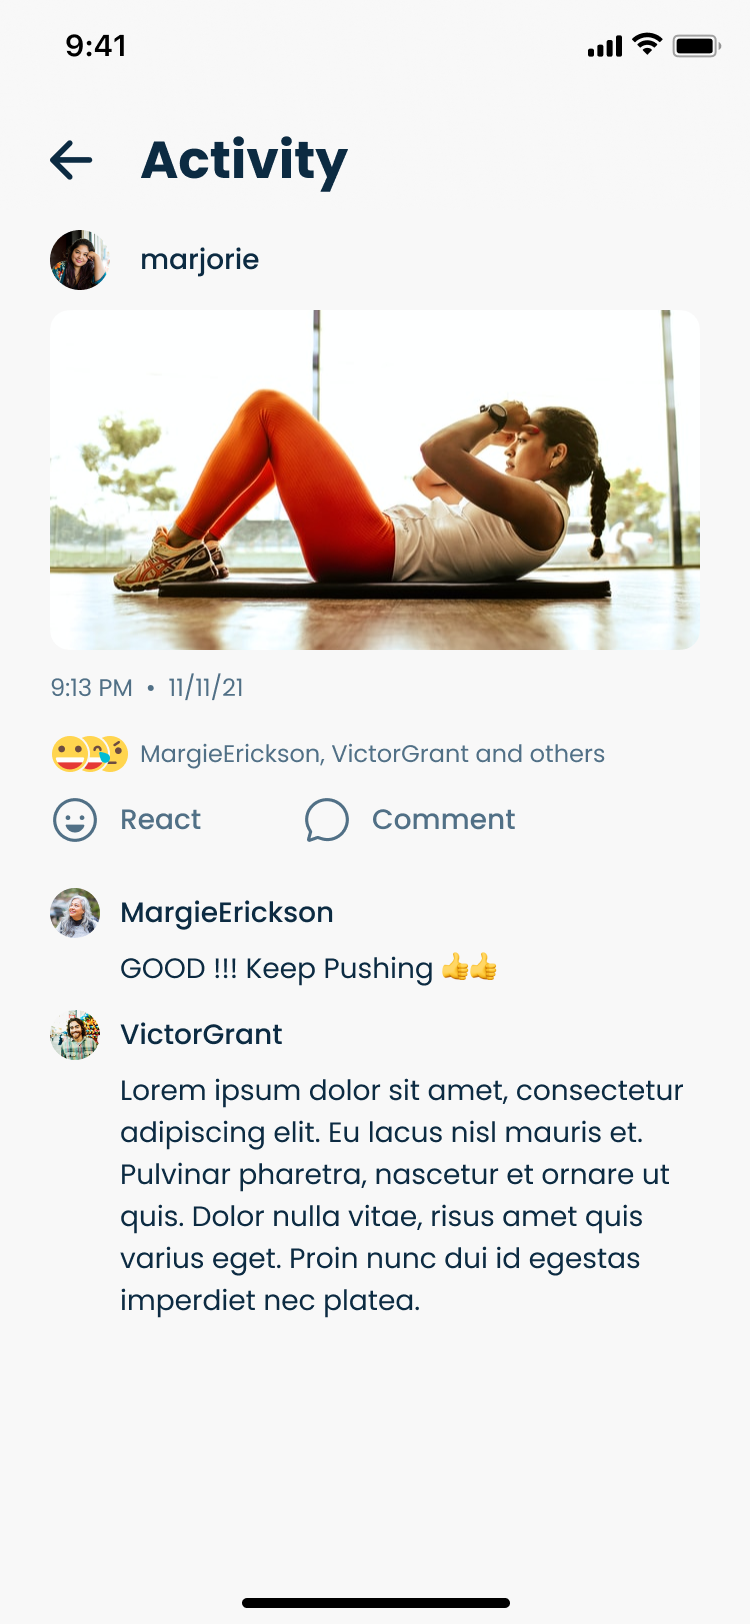
\includegraphics[height=10cm]{chapter_3/ui/Social/Activity.png}
    \caption{หน้ากิจกรรมของผู้ใช้}
\end{figure}
\begin{figure}
    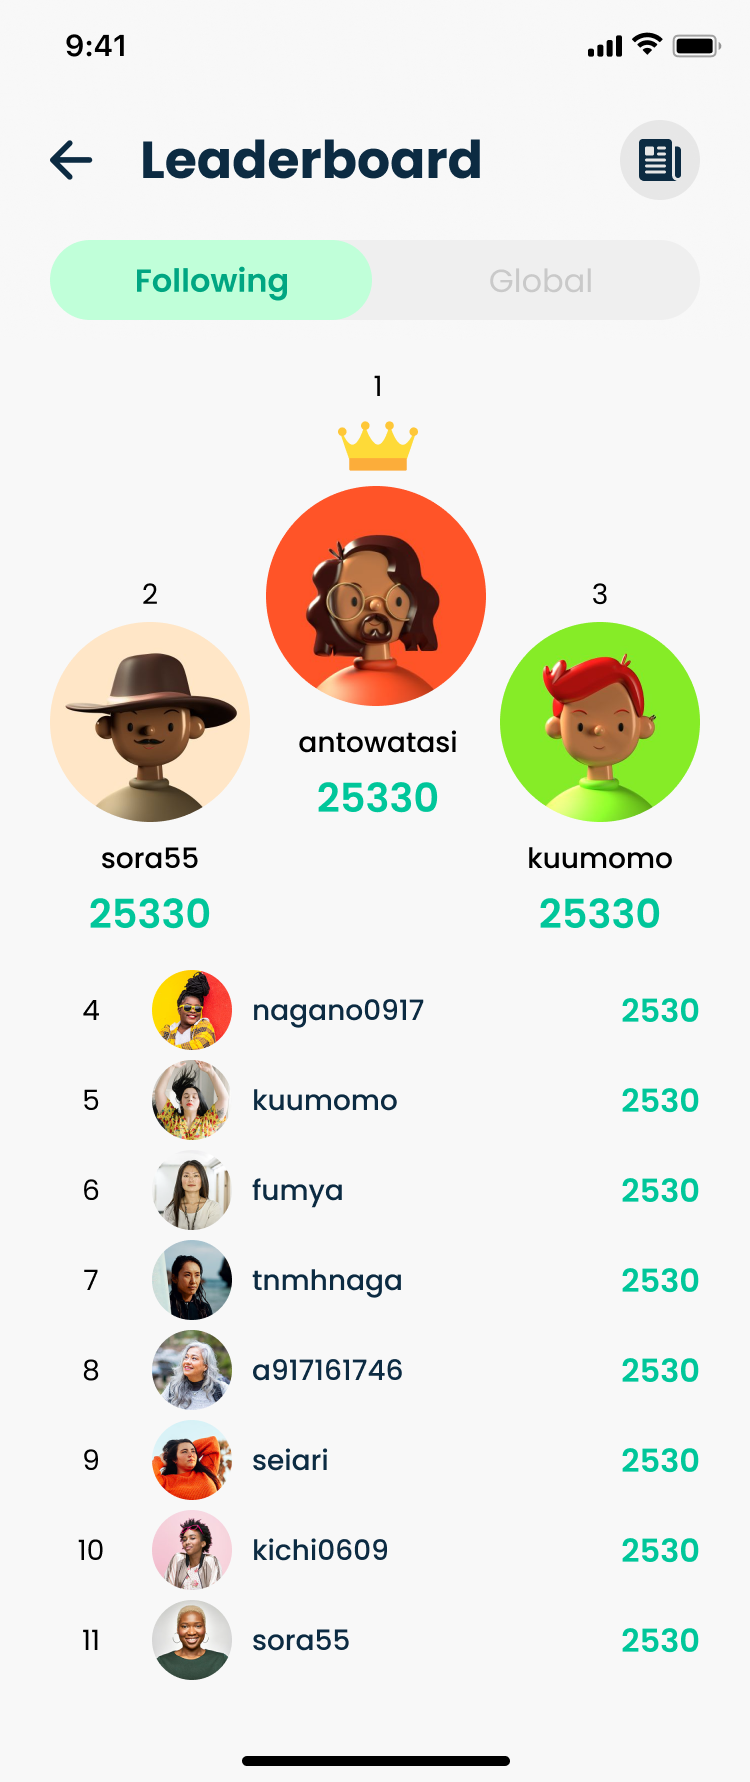
\includegraphics[height=10cm]{chapter_3/ui/Social/Leaderboard.png}
    \caption{หน้าตารางคะแนน Leaderboard}
\end{figure}

\subsection{หน้าข่าวสาร}
หน้าข่าวสารของแอปพลิเคชัน ซึ่งจะให้ผู้ใช้สามารถดูข่าวสารด้านการออกกำลังกายได้ และสามารถกดปุ่มชื่นชอบบทความได้
\begin{figure}
    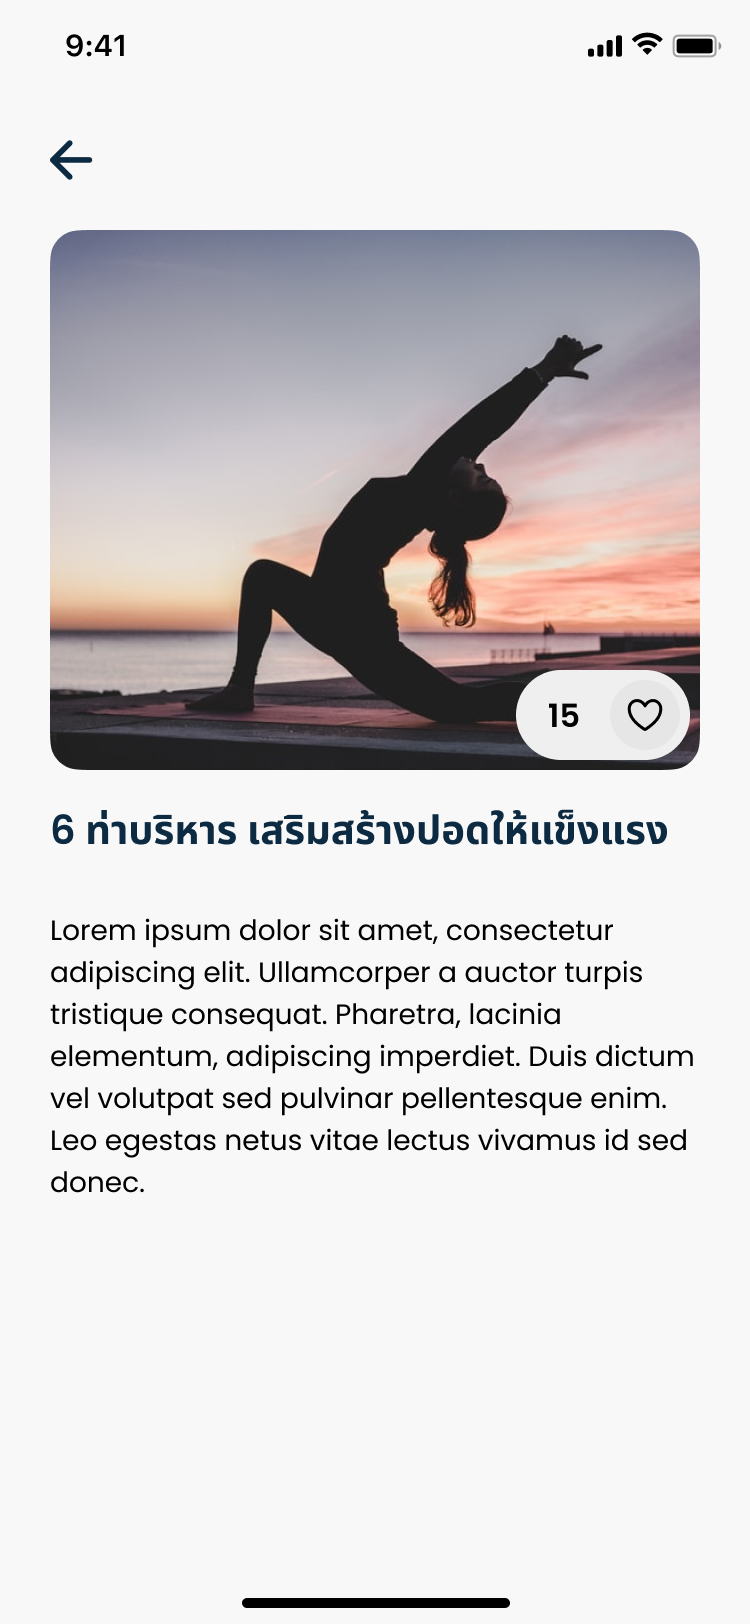
\includegraphics[height=10cm]{chapter_3/ui/News.png}
    \caption{หน้าข่าวสารของแอปพลิเคชัน}
\end{figure}

\subsection{หน้าการออกกำลังกาย}
หน้าการออกกำลังกาย ในหน้าแรกจะแสดงรายละเอียดคอร์ส รวมถึงคะแนนจากผู้ใช้ ระยะเวลาที่ใช้ และระดับความยากของคอร์ส เมื่อผู้ใช้กดปุ่มเริ่มการออกกำลังกาย ระบบจะแนะนำให้ผู้ใช้ทำท่าทางตามที่กำหนด โดยจะมีรายละเอียดแสดงอยู่ทางด้านบน และจะมีการแสดงข้อความแนะนำการปรับปรุงท่าทางการออกกำลังกายให้แก่ผู้ใช้
\begin{figure}
    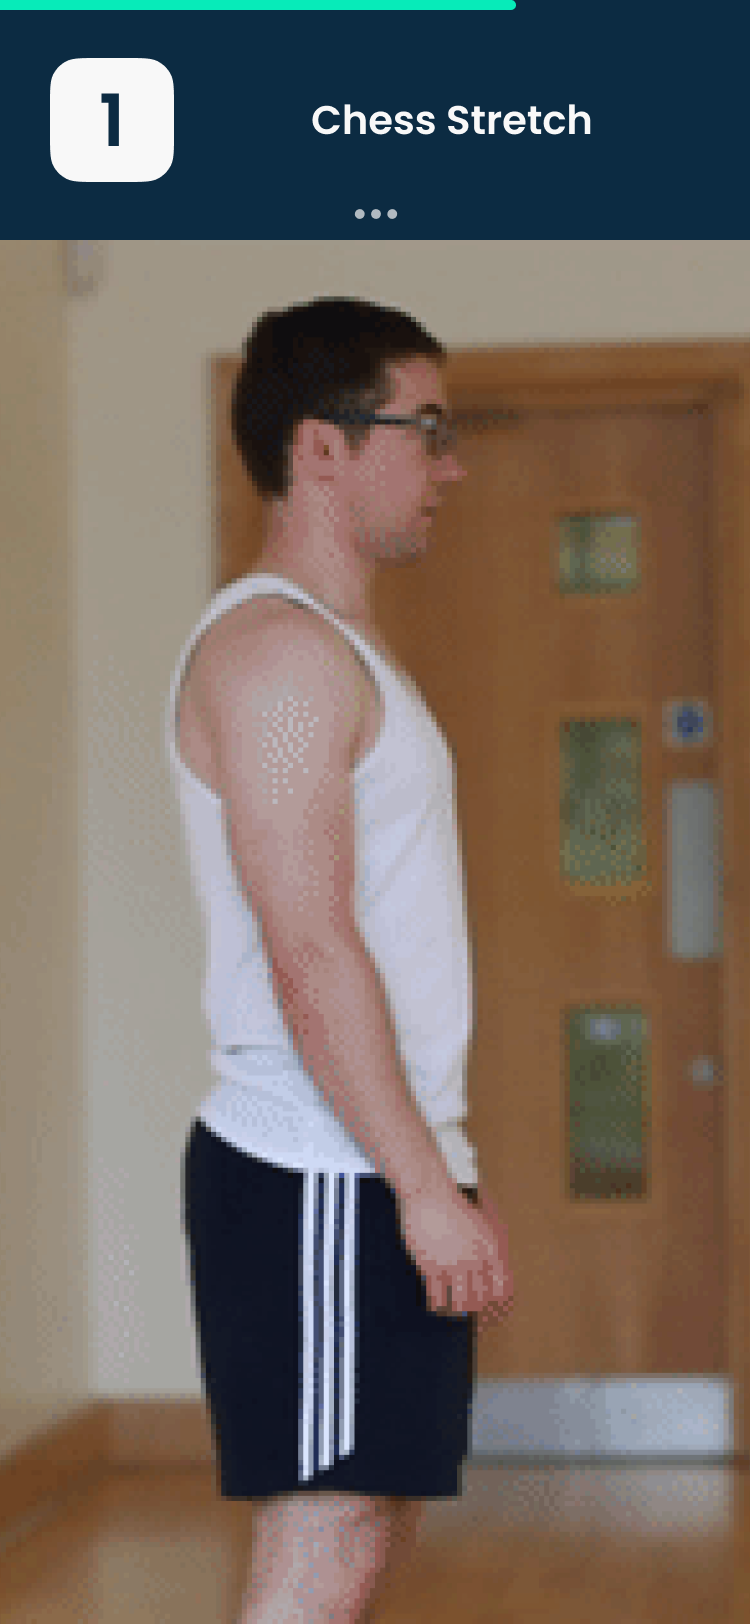
\includegraphics[height=10cm]{chapter_3/ui/Exercise/Step Begin.png}
    \caption{หน้าการสอนท่าทางให้แก่ผู้ใช้}
\end{figure}

\begin{figure}
    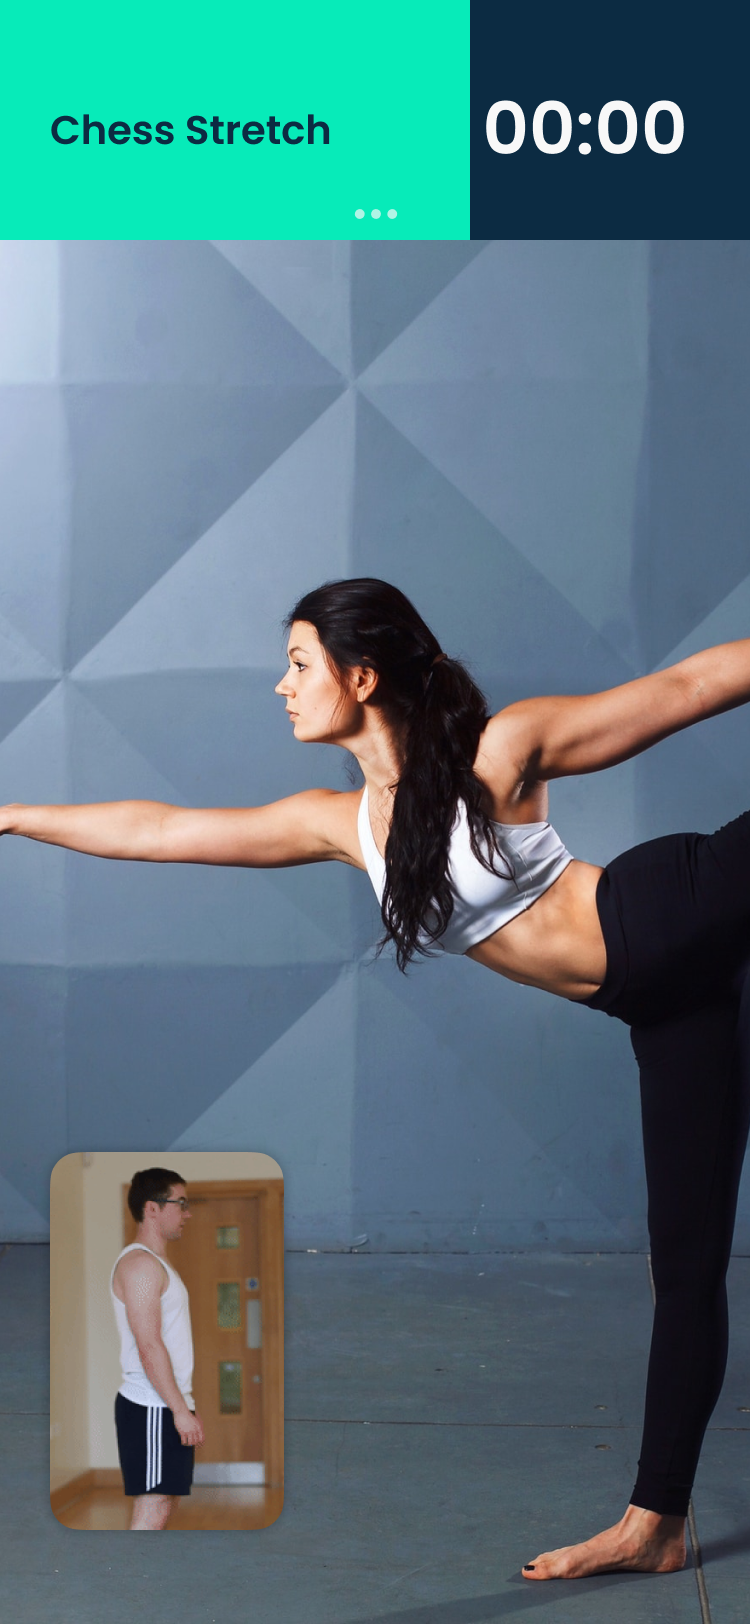
\includegraphics[height=10cm]{chapter_3/ui/Exercise/Step Counting.png}
    \caption{หน้าการออกกำลังกายที่จับเวลาให้ผู้ใช้ออกท่าทางค้างไว้ในเวลาที่กำหนด}
\end{figure}

\begin{figure}
    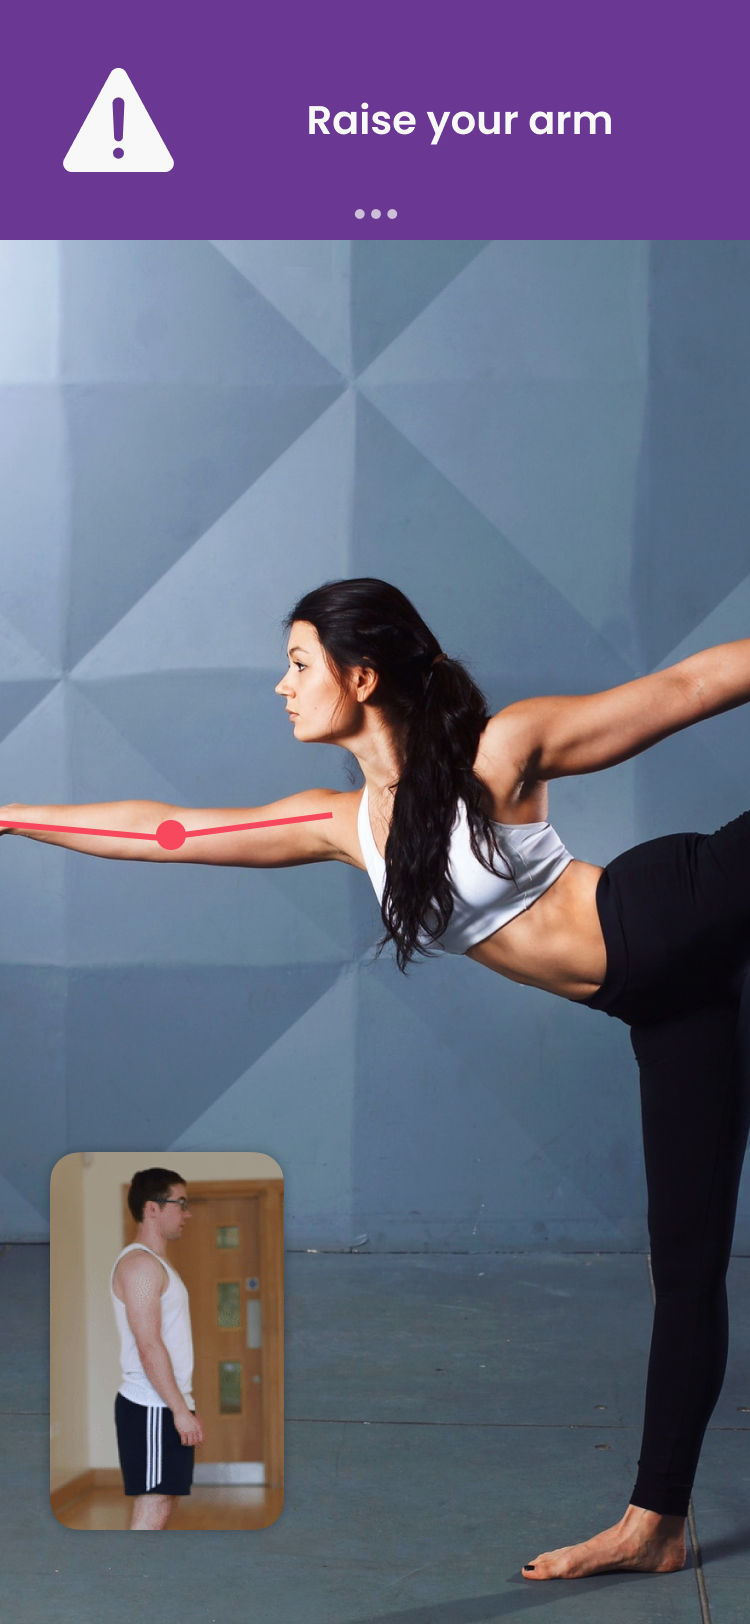
\includegraphics[height=10cm]{chapter_3/ui/Exercise/Warning.png}
    \caption{หน้าการแนะนำการปรับปรุงท่าทางให้แก่ผู้ใช้}
\end{figure}

\begin{figure}
    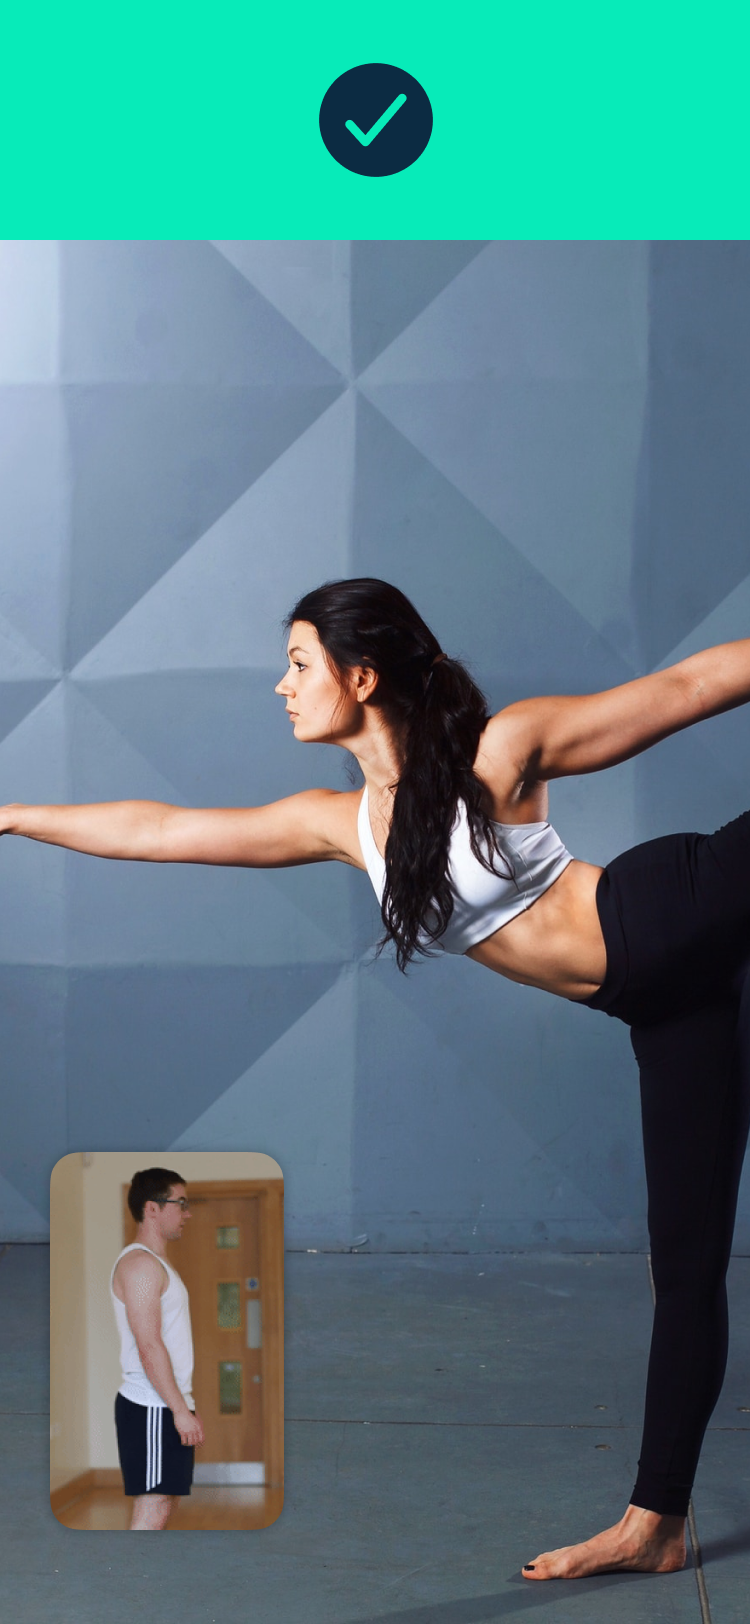
\includegraphics[height=10cm]{chapter_3/ui/Exercise/Step Finish.png}
    \caption{หน้าเมื่อเสร็จสิ้นการออกกำลังกาย}
\end{figure}

\subsection{หน้าบัญชีผู้ใช้}
หน้าบัญชีของผู้ใช้ ให้ผู้ใช้สามารถดูข้อมูลส่วนตัวของตนเองได้ รวมถึงดูเหรียญรางวัลเสมือนของตนเองได้

\begin{figure}
    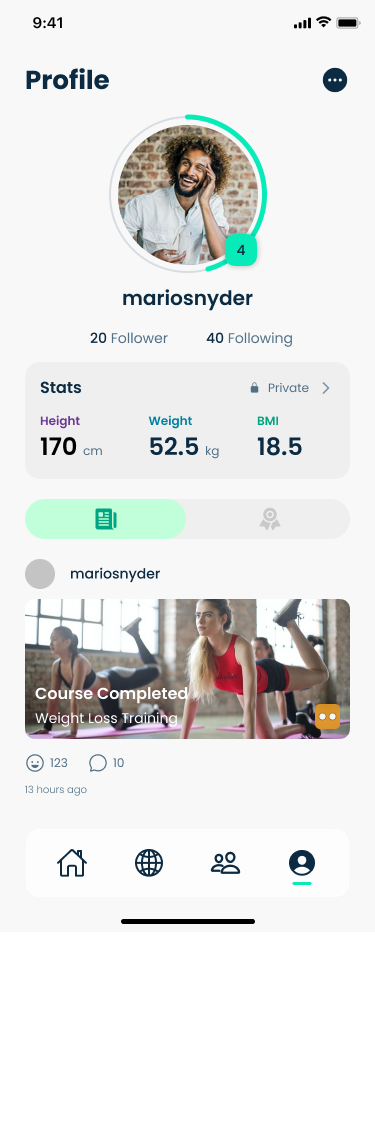
\includegraphics[height=10cm]{chapter_3/ui/Profile.png}
    \caption{หน้าบัญชีของผู้ใช้}
\end{figure}


\clearpage

\section{การออกแบบส่วนโครงสร้างระบบฐานข้อมูล (Database Schema)}
% TODO: Change the schema
การออกแบบส่วนโครงสร้างระบบฐานข้อมูล (Database Schema) ดังนี้
\begin{figure}
    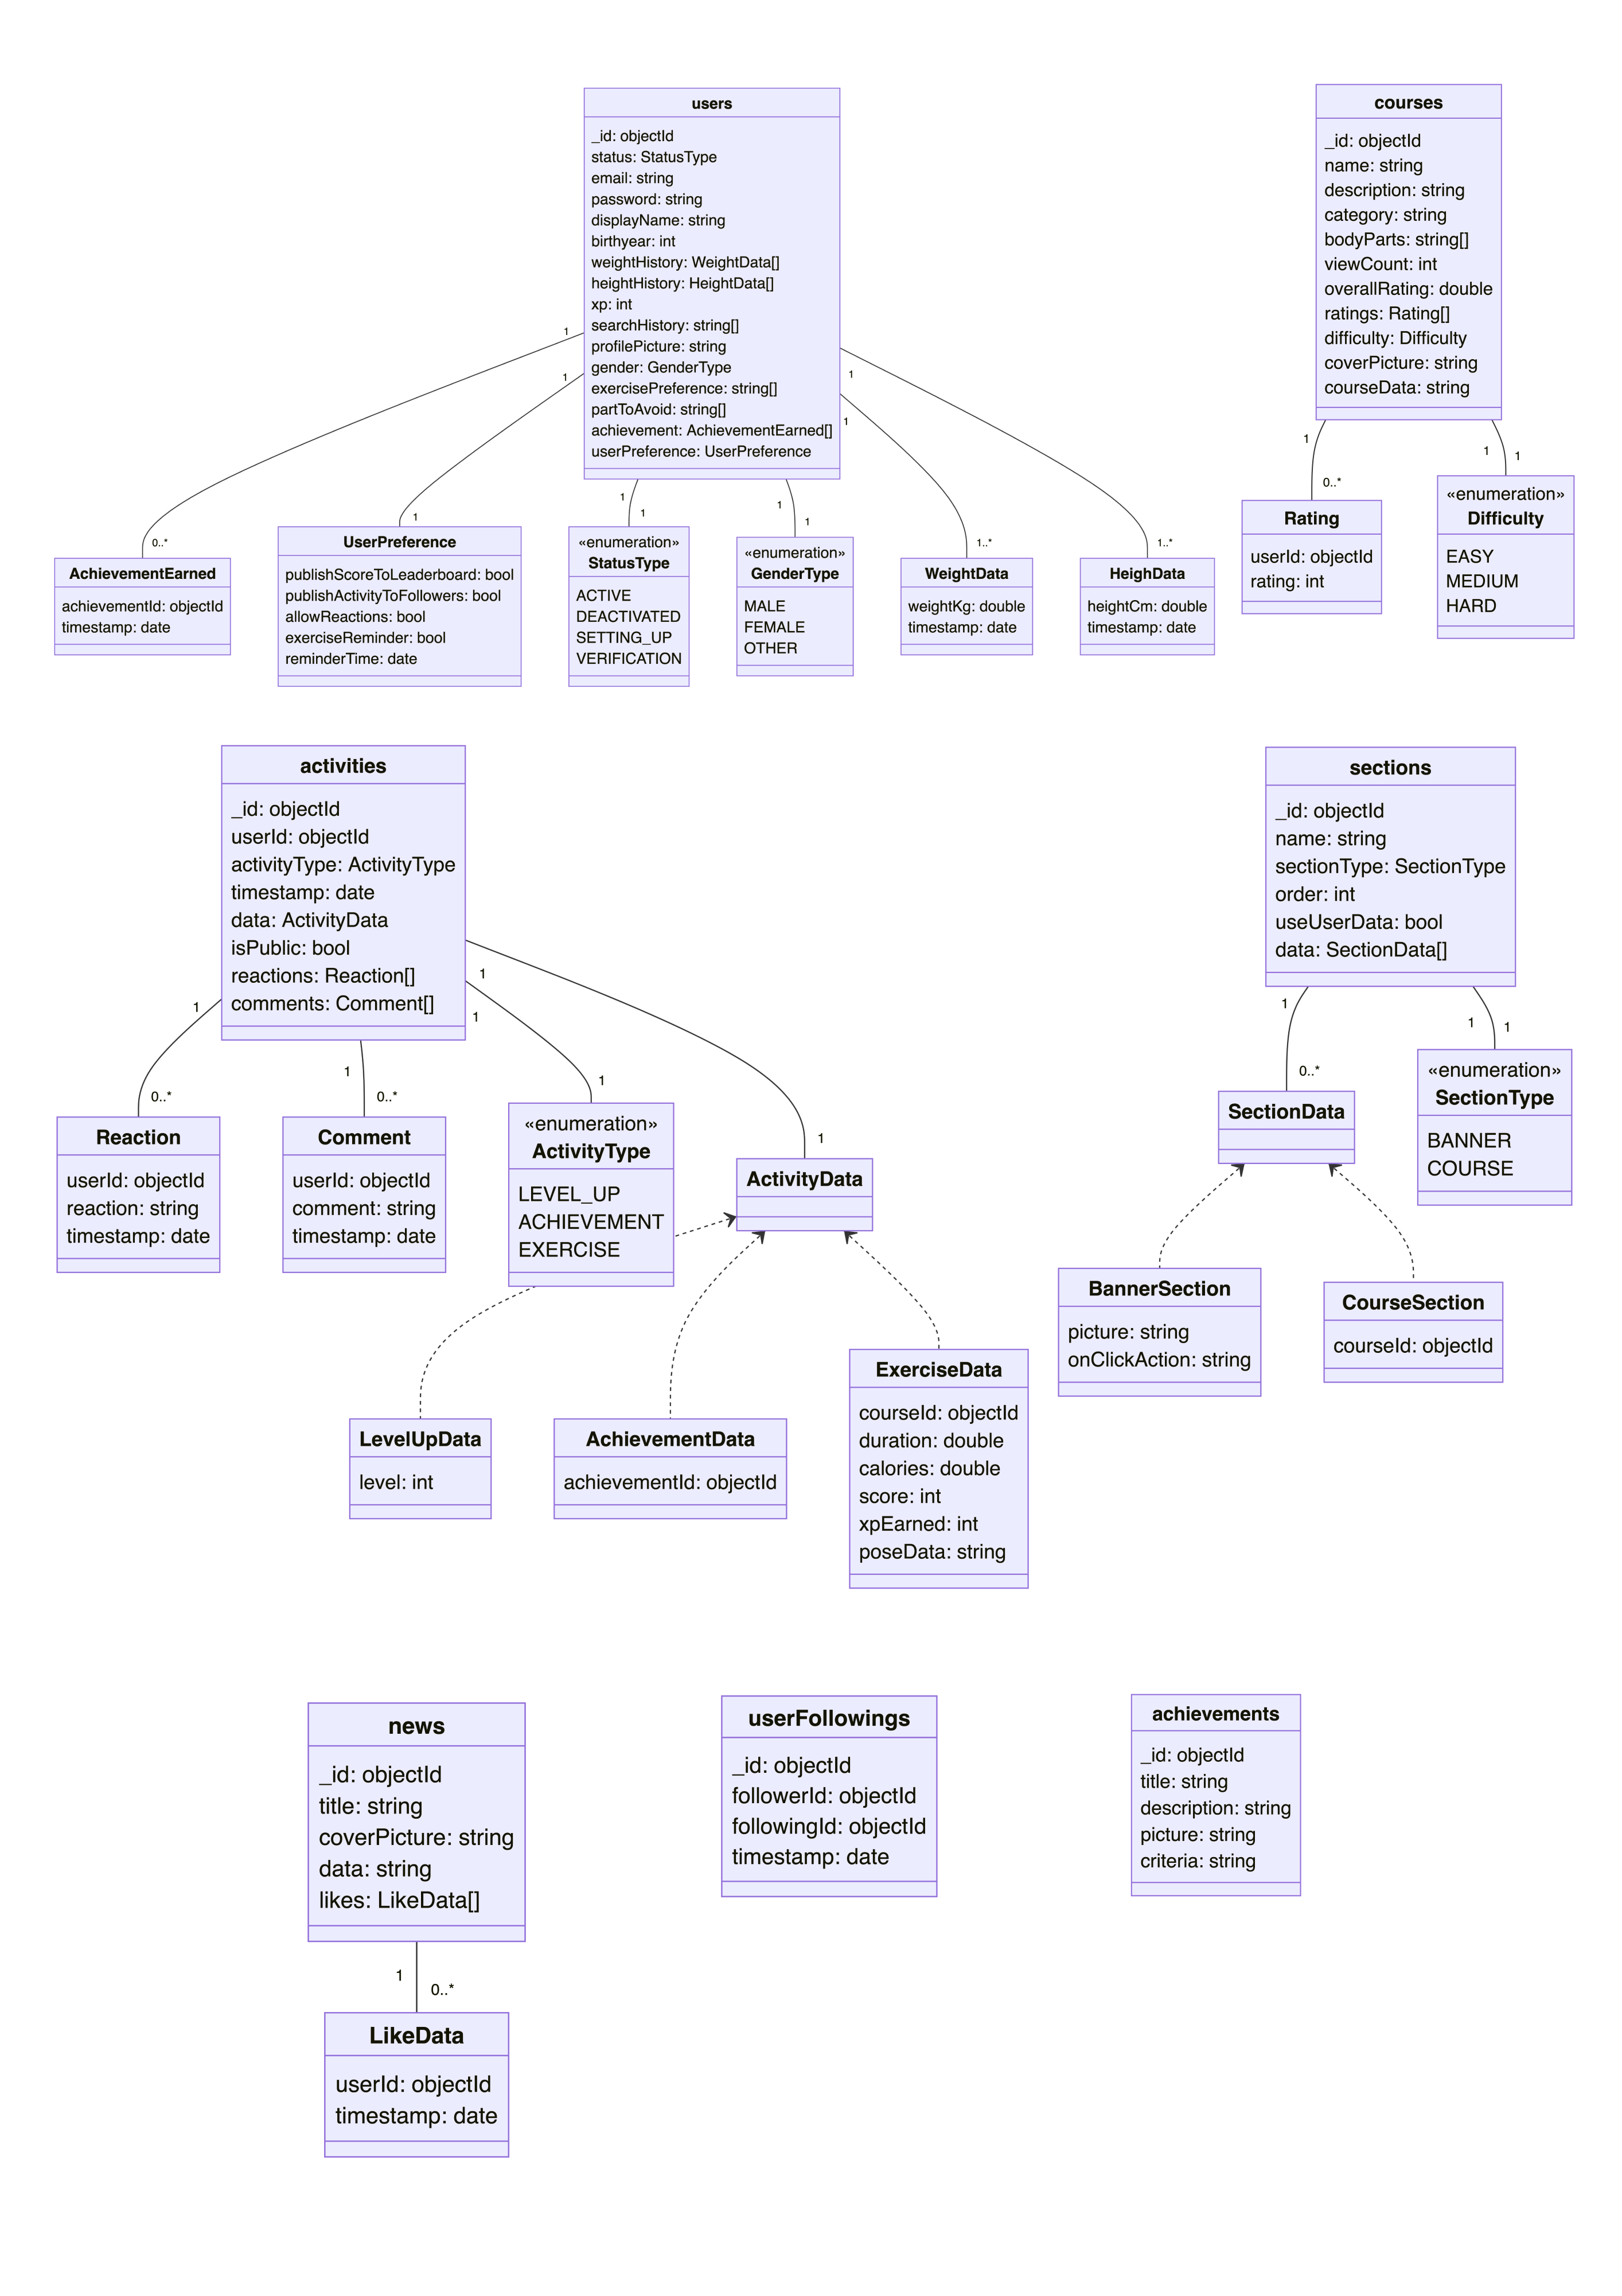
\includegraphics[width=\textwidth]{chapter_3/database.png}
    \caption{การออกแบบโครงสร้างฐานข้อมูล}
    \label{fig:db-schema}
\end{figure}
\clearpage
การออกแบบฐานข้อมูลตามรูปที่ \ref{fig:db-schema} มีรายละเอียดดังต่อไปนี้

\begin{table}
    \caption{รายละเอียดฐานข้อมูลในคอลเล็กชัน users}
    \begin{tabularx}{\textwidth}{ | l | l | X | }
        \hline
        \bf ชื่อแอตทริบิวต์ & \bf ชนิดตัวแปร & \bf รายละเอียด \\\hline
        \_ id & objectId & ID ของ document ใน collection users\\\hline
        status & StatusType & สถานะของบัญชีผู้ใช้\\\hline
        email & string & อีเมลของผู้ใช้\\\hline
        password & string & รหัสผ่านของผู้ใช้\\\hline
        displayName & string & ชื่อ Display Name ของผู้ใช้\\\hline
        birthyear & int & ปีเกิดของผู้ใช้\\\hline
        weightHistory & WeightData[] & ประวัติน้ำหนักของผู้ใช้\\\hline
        heightHistory & HeightData[] & ประวัติส่วนสูงของผู้ใช้\\\hline
        xp & int & คะแนนของผู้ใช้\\\hline
        level & int & ขั้น (Level) ของผู้ใช้\\\hline
        profilePicture & string & URL รูปภาพโปรไฟล์ของผู้ใช้\\\hline
        gender & GenderType & เพศของผู้ใช้\\\hline
        exercisePreference & string[] & รายการประเภทการออกกำลังกายที่ชอบ\\\hline
        partToAvoid & string[] & รายการสัดส่วนของผู้ใช้ที่ต้องการหลีกเลี่ยง\\\hline
    \end{tabularx}
\end{table}

\begin{table}
    \caption{รายละเอียดชนิดตัวแปร AchievementEarned}
    \begin{tabularx}{\textwidth}{ | l | l | X | }
        \hline
        \bf ชื่อแอตทริบิวต์ & \bf ชนิดตัวแปร & \bf รายละเอียด \\\hline
        achievementId & objectId & ID ของเหรียญรางวัลเสมือน\\\hline
        timestamp & date & วันและเวลาที่ผู้ใช้ได้รับเหรียญ\\\hline 
    \end{tabularx}
\end{table}

\begin{table}
    \caption{รายละเอียดชนิดตัวแปร UserPreference}
    \begin{tabularx}{\textwidth}{ | l | l | X | }
        \hline
        \bf ชื่อแอตทริบิวต์ & \bf ชนิดตัวแปร & \bf รายละเอียด \\\hline
        publishScoreToLeaderboard & bool & เผยแพร่คะแนนของผู้ใช้บนตารางลีดเดอร์บอร์ด\\\hline
        publishActivityToFollowers & bool & เผยแพร่กิจกรรมของผู้ใช้ไปยังคนที่กำลังติดตามผู้ใช้\\\hline
        allowReactions & bool & ให้ผู้อื่นสามารถกด Reaction กับกิจกรรมได้\\\hline
        exerciseReminder & bool & การแจ้งเตือนให้ออกกำลังกาย\\\hline
        reminderTime & date & เวลาที่ผู้ใช้ต้องการให้เตือนเพือออกกำลังกาย\\\hline
    \end{tabularx}
\end{table}

\begin{table}
    \caption{รายละเอียด Enumeration StatusType}
    \begin{tabularx}{\textwidth}{ | l | X | }
        \hline
        \bf ชื่อแอตทริบิวต์ & \bf รายละเอียด \\\hline
        ACTIVE & บัญชีผู้ใช้มีสถานะปกติ\\\hline
        DEACTIVATED & บัญชีผู้ใช้มีสถานะปิดบัญชี\\\hline
        SETTING\_UP & บัญชีผู้ใช้มีสถานะกำลังอยู่ในขั้นตอนการตั้งค่าผู้ใช้ใหม่\\\hline
        VERIFICATION & บัญชีผู้ใช้มีสถานะกำลังรอการยืนยันอีเมล\\\hline
    \end{tabularx}
\end{table}

\begin{table}
    \caption{รายละเอียด Enumeration GenderType}
    \begin{tabularx}{\textwidth}{ | l | X | }
        \hline
        \bf ชื่อแอตทริบิวต์ & \bf รายละเอียด \\\hline
        MALE & เพศของผู้ใช้คือเพศชาย\\\hline
        FEMALE & เพศของผู้ใช้คือเพศหญิง\\\hline
        OTHER & เพศของผู้ใช้คืออื่น ๆ\\\hline
    \end{tabularx}
\end{table}

\begin{table}
    \caption{รายละเอียดชนิดตัวแปร WeightData}
    \begin{tabularx}{\textwidth}{ | l | l | X | }
        \hline
        \bf ชื่อแอตทริบิวต์ & \bf ชนิดตัวแปร & \bf รายละเอียด \\\hline
        weightKg & double & น้ำหนักของผู้ใช้ (หน่วยกิโลกรัม)\\\hline
        timestamp & date & วันที่และเวลาที่ผู้ใช้กรอกข้อมูล\\\hline
    \end{tabularx}
\end{table}

\begin{table}
    \caption{รายละเอียดชนิดตัวแปร HeightData}
    \begin{tabularx}{\textwidth}{ | l | l | X | }
        \hline
        \bf ชื่อแอตทริบิวต์ & \bf ชนิดตัวแปร & \bf รายละเอียด \\\hline
        heightCm & double & ส่วนสูงของผู้ใช้ (หน่วยเซนติเมตร)\\\hline
        timestamp & date & วันที่และเวลาที่ผู้ใช้กรอกข้อมูล\\\hline
    \end{tabularx}
\end{table}

\begin{table}
    \caption{รายละเอียดฐานข้อมูลใน collection courses}
    \begin{tabularx}{\textwidth}{ | l | l | X | }
        \hline
        \bf ชื่อแอตทริบิวต์ & \bf ชนิดตัวแปร & \bf รายละเอียด \\\hline
        \_id & objectId & ID ของ document ใน collection courses\\\hline
        name & string & ชื่อคอร์ส\\\hline
        description & string & คำอธิบายของคอร์ส\\\hline
        category & string & หมวดหมู่คอร์ส\\\hline
        bodyParts & string[] & ส่วนของร่างกายที่ต้องใช้\\\hline
        viewCount & int & จำนวนการเข้าดูคอร์สนี้\\\hline
        rating & Rating[] & รายการของผู้ใช้ที่ให้คะแนนกับคอร์สนี้\\\hline
        difficulty & Difficulty & ความยาก-ง่ายของคอร์ส\\\hline
        coverPicture & string & URL รูปภาพหน้าปกคอร์ส\\\hline
        courseData & string & URL ไฟล์ข้อมูลท่าทางการออกกำลังกาย\\\hline
    \end{tabularx}
\end{table}

\begin{table}
    \caption{รายละเอียดชนิดตัวแปร Rating}
    \begin{tabularx}{\textwidth}{ | l | l | X | }
        \hline
        \bf ชื่อแอตทริบิวต์ & \bf ชนิดตัวแปร & \bf รายละเอียด \\\hline
        userId & objectId & ID ของผู้ใช้ที่ให้คะแนน\\\hline
        rating & int & คะแนนที่ผู้ใช้ให้\\\hline
    \end{tabularx}
\end{table}

\begin{table}
    \caption{รายละเอียด Enumeration Difficulty}
    \begin{tabularx}{\textwidth}{ | l | X | }
        \hline
        \bf ชื่อแอตทริบิวต์ & \bf รายละเอียด \\\hline
        EASY & คอร์สระดับง่าย\\\hline
        MEDIUM & คอร์สระดับปานกลาง\\\hline
        HARD & คอร์สระดับยาก\\\hline
    \end{tabularx}
\end{table}

\begin{table}
    \caption{รายละเอียดฐานข้อมูลในคอลเล็กชัน achievements}
    \begin{tabularx}{\textwidth}{ | l | l | X | }
        \hline
        \bf ชื่อแอตทริบิวต์ & \bf ชนิดตัวแปร & \bf รายละเอียด \\\hline
        \_id & objectId & ID ของเหรียญรางวัลเสมือน\\\hline
        title & string & ชื่อของเหรียญรางวัลเสมือน\\\hline
        description & string & คำอธิบายเหรียญรางวัลเสมือน\\\hline
        picture & string & รูปภาพของเหรียญรางวัลเสมือน\\\hline
        criteria & string[] & รายการเกณฑ์ต่าง ๆ ของเหรียญรางวัลเสมือน\\\hline
    \end{tabularx}
\end{table}

\begin{table}
    \caption{รายละเอียดฐานข้อมูลในคอลเล็กชัน activities}
    \begin{tabularx}{\textwidth}{ | l | l | X | }
        \hline
        \bf ชื่อแอตทริบิวต์ & \bf ชนิดตัวแปร & \bf รายละเอียด \\\hline
        \_id & objectId & ID ของกิจกรรม\\\hline
        userId & objectId & ID ของผู้ใช้ที่เป็นผู้ทำกิจกรรม\\\hline
        activityType & ActivityType & ประเภทของกิจกรรม\\\hline
        timestamp & date & วันที่และเวลาที่ทำกิจกรรม\\\hline
        data & ActivityData & ข้อมูลรายละเอียดของกิจกรรม\\\hline
        isPublic & bool & ให้กิจกรรมนี้สามารถให้ผู้ที่ติดตามมองเห็นได้หรือไม่\\\hline
        reactions & Reaction[] & รายการผู้ใช้ที่กดแสดงความรู้สึก (Reaction) ต่อกิจกรรมนี้\\\hline
        comments & Comment[] & รายการที่ผู้ใช้แสดงความคิดเห็น (Comment) ต่อกิจกรรมนี้\\\hline
    \end{tabularx}
\end{table}

\begin{table}
    \caption{รายละเอียดชนิดตัวแปร LevelUpData}
    \begin{tabularx}{\textwidth}{ | l | l | X | }
        \hline
        \bf ชื่อแอตทริบิวต์ & \bf ชนิดตัวแปร & \bf รายละเอียด \\\hline
        level & int & ระดับ (Level) ที่ผู้ใช้ได้รับ\\\hline
    \end{tabularx}
\end{table}

\begin{table}
    \caption{รายละเอียดชนิดตัวแปร ExerciseData}
    \begin{tabularx}{\textwidth}{ | l | l | X | }
        \hline
        \bf ชื่อแอตทริบิวต์ & \bf ชนิดตัวแปร & \bf รายละเอียด \\\hline
        courseId & objectId & ID ของคอร์สที่ผู้ใช้ได้ออกกำลังกาย\\\hline
        duration & double & ระยะเวลาที่ผู้ใช้เข้าคอร์ส (นาที)\\\hline
        calories & double & จำนวนแคลอรี่ที่ผู้ใช้ได้เผาผลาญไป\\\hline
        score & int & คะแนนความถูกต้องในการออกกำลังกายของผู้ใช้ (เป็นช่วงจาก 0 - 100)\\\hline
        xpEarned & int & คะแนนที่ผู้ใช้ได้รับ\\\hline
        poseData & string & URL ไฟล์ข้อมูลท่าทางของผู้ใช้\\\hline
    \end{tabularx}
\end{table}

\begin{table}
    \caption{รายละเอียด Enumeration ActivityType}
    \begin{tabularx}{\textwidth}{ | l | X | }
        \hline
        \bf ชื่อแอตทริบิวต์ & \bf รายละเอียด \\\hline
        LEVEL\_UP & กิจกรรม ประเภทการเลื่อนระดับ\\\hline
        ACHIEVEMENT & กิจกรรม ประเภทที่ได้รับเหรียญรางวัลเสมือน\\\hline
        EXERCISE & กิจกรรม ประเภทการออกกำลังกาย\\\hline
    \end{tabularx}
\end{table}

\begin{table}
    \caption{รายละเอียดชนิดตัวแปร Reaction}
    \begin{tabularx}{\textwidth}{ | l | l | X | }
        \hline
        \bf ชื่อแอตทริบิวต์ & \bf ชนิดตัวแปร & \bf รายละเอียด \\\hline
        \_id & objectId & ID ของกิจกรรม\\\hline
        userId & objectId & ID ของผู้ใช้ที่ได้แสดงความรู้สึก (Reaction)\\\hline
        reaction & string & ชื่อความรู้สึก (Reaction)\\\hline
        timestamp & date & วันที่และเวลาที่ได้กดแสดงความรู้สึก (Reaction)\\\hline
    \end{tabularx}
\end{table}

\begin{table}
    \caption{รายละเอียดชนิดตัวแปร Comment}
    \begin{tabularx}{\textwidth}{ | l | l | X | }
        \hline
        \bf ชื่อแอตทริบิวต์ & \bf ชนิดตัวแปร & \bf รายละเอียด \\\hline
        \_id & objectId & ID ของกิจกรรม\\\hline
        userId & objectId & ID ของผู้ใช้ที่ได้แสดงความคิดเห็น\\\hline
        comment & string & ความคิดเห็นของผู้ใช้\\\hline
        timestamp & date & วันที่และเวลาที่ได้แสดงความคิดเห็น\\\hline
    \end{tabularx}
\end{table}

\begin{table}
    \caption{รายละเอียดฐานข้อมูลในคอลเล็กชัน news}
    \begin{tabularx}{\textwidth}{ | l | l | X | }
        \hline
        \bf ชื่อแอตทริบิวต์ & \bf ชนิดตัวแปร & \bf รายละเอียด \\\hline
        \_id & objectId & ID ของข่าวสาร\\\hline
        title & string & หัวเรื่องของข่าวสาร\\\hline
        coverPicture & string & URL รูปภาพหน้าปก\\\hline
        data & string & URL ไฟล์ข้อมูลของข่าวสาร\\\hline
        likes & LikeData[] & รายการผู้ที่กดชื่นชอบข่าว\\\hline
    \end{tabularx}
\end{table}

\begin{table}
    \caption{รายละเอียดชนิดตัวแปร LikeData}
    \begin{tabularx}{\textwidth}{ | l | l | X | }
        \hline
        \bf ชื่อแอตทริบิวต์ & \bf ชนิดตัวแปร & \bf รายละเอียด \\\hline
        userId & objectId & ID ของผู้ใช้\\\hline
        timestamp & date & วันและเวลาที่ผู้ใช้กดชื่นชอบ\\\hline
    \end{tabularx}
\end{table}

\begin{table}
    \caption{รายละเอียดฐานข้อมูลในคอลเล็กชัน sections}
    \noindent ใช้ในการเก็บข้อมูลส่วนต่าง ๆ ในหน้าหลัก (Home) ที่จะมีการแนะนำคอร์สต่าง ๆ
    \begin{tabularx}{\textwidth}{ | l | l | X | }
        \hline
        \bf ชื่อแอตทริบิวต์ & \bf ชนิดตัวแปร & \bf รายละเอียด \\\hline
        \_id & objectId & ID ของส่วน\\\hline
        name & string & ชื่อของส่วนนี้\\\hline
        sectionType & SectionType & ประเภทของส่วน\\\hline
        order & int & ลำดับของส่วนบนหน้าหลัก\\\hline
        useUserData & bool & นำข้อมูลของผู้ใช้มาประกอบการแนะนำหรือไม่\\\hline
        data & SectionData[] & ข้อมูลของส่วน\\\hline
    \end{tabularx}
\end{table}

\begin{table}
    \caption{รายละเอียดชนิดคลาส BannerSection}
    \noindent ใช้ในการเก็บข้อมูลส่วนต่าง ๆ ในหน้าหลัก (Home) ที่จะมีการแนะนำคอร์สต่าง ๆ
    \begin{tabularx}{\textwidth}{ | l | l | X | }
        \hline
        \bf ชื่อแอตทริบิวต์ & \bf ชนิดตัวแปร & \bf รายละเอียด \\\hline
        picture & string & URL ไฟล์รูปภาพ\\\hline
        onClickAction & string & กำหนดการกระทำเมื่อผู้ใช้กดไปยัง Banner\\\hline
    \end{tabularx}
\end{table}

\begin{table}
    \caption{รายละเอียดชนิดคลาส CourseSection}
    \begin{tabularx}{\textwidth}{ | l | l | X | }
        \hline
        \bf ชื่อแอตทริบิวต์ & \bf ชนิดตัวแปร & \bf รายละเอียด \\\hline
        courseId & objectId & คอร์สที่แนะนำ\\\hline
    \end{tabularx}
\end{table}

\begin{table}
    \caption{รายละเอียด Enumeration SectionType}
    \begin{tabularx}{\textwidth}{ | l | X | }
        \hline
        \bf ชื่อแอตทริบิวต์ & \bf รายละเอียด \\\hline
        BANNER & ส่วนเป็นแบบ Banner\\\hline
        COURSE & ส่วนเป็นแบบ Course\\\hline
    \end{tabularx}
\end{table}

\begin{table}
    \caption{รายละเอียดฐานข้อมูลในคอลเล็กชัน userFollowings}
    \begin{tabularx}{\textwidth}{ | l | l | X | }
        \hline
        \bf ชื่อแอตทริบิวต์ & \bf ชนิดตัวแปร & \bf รายละเอียด \\\hline
        \_id & objectId & ID ของรายการบันทึกการติดตามของผู้ใช้\\\hline
        followerId & objectId & ID ของผู้ใช้ที่กดติดตาม\\\hline
        followingId & objectId & ID ของผู้ใช้ที่ถูกติดตาม\\\hline
        timestamp & date & วันและเวลาที่ผู้ใช้ได้กดติดตาม\\\hline
    \end{tabularx}
\end{table}

\clearpage


\section{การออกแบบส่วนการวิเคราะห์ ตรวจสอบ และแนะนำท่าทางของผู้ใช้}
ในการออกแบบส่วนการวิเคราะห์ ตรวจสอบ และแนะนำท่าทางของผู้ใช้ จะแสดงเป็นแผนภาพการทำงานระหว่างระบบต่าง ๆ ได้ ดังนี้
\begin{figure}
    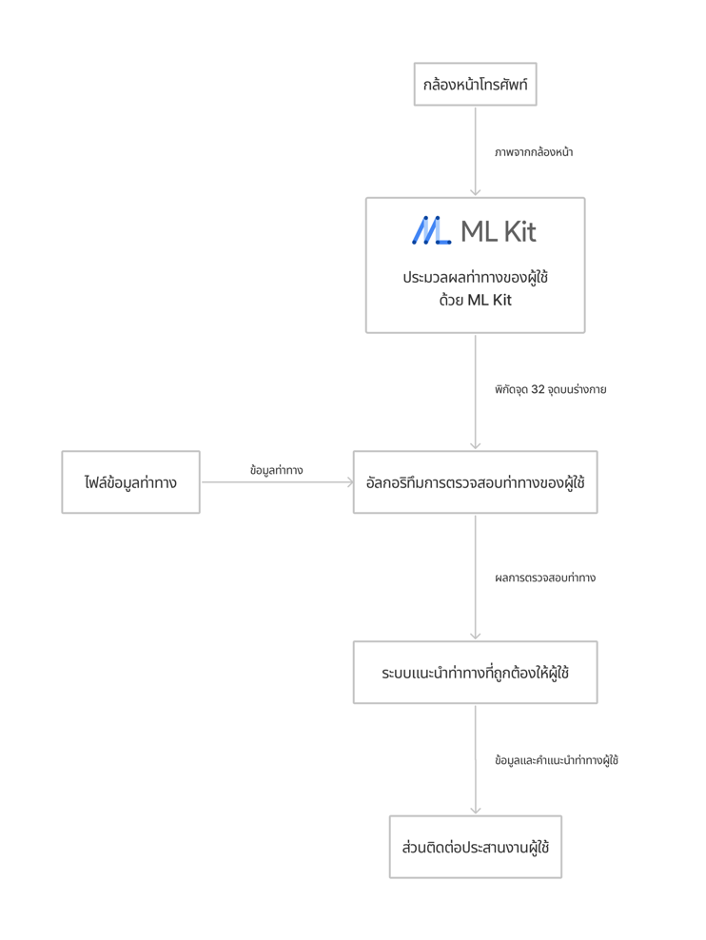
\includegraphics[width=\textwidth - 2cm]{chapter_3/pose overview.png}
    \caption{ภาพรวมระบบการวิเคราะห์ ตรวจสอบ และแนะนำท่าทางของผู้ใช้}
\end{figure}
จากแผนภาพข้างต้น สามารถอธิบายออกเป็นส่วนต่าง ๆ ซึ่งจะแบ่งออกเป็น 4 ส่วน คือ ส่วนการประมวลผลท่าทางของผู้ใช้ด้วย ML Kit, ส่วนไฟล์ข้อมูลท่าทาง, ส่วนอัลกอริทึมการตรวจสอบท่าทางของผู้ใช้ และส่วนระบบแนะนำท่าทางที่ถูกต้องให้ผู้ใช้

\subsection{ส่วนการประมวลผลท่าทางของผู้ใช้ด้วย ML Kit}
สำหรับระบบการวิเคราะห์ท่าทาง จะใช้ API ของ ML Kit ในการตรวจจับท่าทางของผู้ใช้ ซึ่งจะได้พิกัดจุดทั้งหมด 32 จุดทั่วร่างกาย
\begin{figure}
    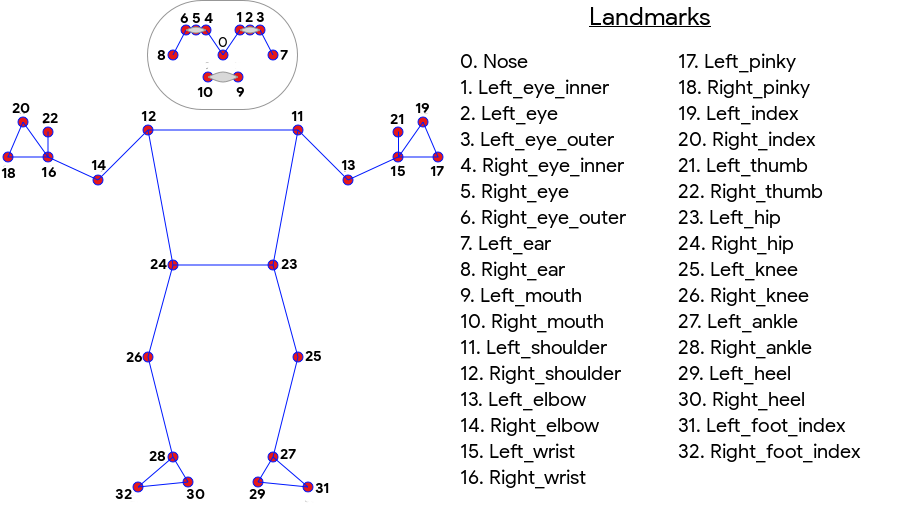
\includegraphics[width=\textwidth]{chapter_3/landmarks-fixed.png}
    \caption{แสดง Landmark จุดบนร่างกายที่ ML Kit สามารถตรวจจับได้}
\end{figure}

\subsection{ส่วนอัลกอริทึมการตรวจสอบท่าทางของผู้ใช้}
ในส่วนของการตรวจสอบท่าทางของผู้ใช้ ระบบจะนำข้อมูลพิกัดจุดที่ได้จากการประมวลผลในขั้นตอนที่แล้วมาใช้ โดยจะใช้ควบคู่กับไฟล์ข้อมูลท่าทางที่จะมีข้อมูลว่าจะต้องตรวจสอบท่าทางในจุดใดบ้าง ซึ่งจะประกอบไปด้วยคำสั่งที่จะให้ตรวจสอบ 2 คำสั่งคือ คำสั่งในการตรวจสอบองศาที่ทำมุมกันของจุดใด ๆ และคำสั่งตรวจสอบจุดใด ๆ ว่าอยู่ใกล้กันกับอีกจุดหนึ่งหรือไม่ โดยจะมีรายละเอียดในการหาผลลัพธ์ ดังนี้
\begin{enumerate}
    \item 	คำสั่งให้ตรวจสอบองศาของจุดที่ทำมุมกัน ในขั้นตอนแรกจะรับจุดทั้งหมด 3 จุด คือ จุด $A,B,C$ ซึ่งจะให้จุด $A$ เป็นจุดเริ่มต้น จากนั้นจึงคำนวณเวกเตอร์สามมิติซึ่งจะได้ออกมาเป็นเวกเตอร์ $\overrightarrow{AB}$ และ เวกเตอร์ $\overrightarrow{AC}$ ดังรูปภาพตัวอย่าง
    \begin{figure}
        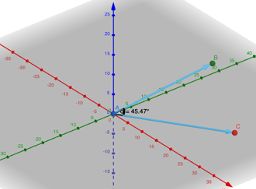
\includegraphics[width=7cm]{chapter_3/vector ex.png}
        \caption{แสดงตัวอย่างการหาเวกเตอร์ที่มีจุด A เป็นจุดร่วม}
    \end{figure}
    จากนั้นจึงหาองศาระหว่างเวกเตอร์ทั้งสองได้ จากสมการ
    \begin{equation}
        \alpha = \arccos{\left( \frac{\overrightarrow{AB} \cdot \overrightarrow{AC}}{|\overrightarrow{AB}| \cdot |\overrightarrow{AC}|} \right)}
    \end{equation}
    และเมื่อได้องศาเรียบร้อยแล้ว จึงจะนำไปตรวจสอบกับค่าที่ได้รับว่าตรงตามที่ได้กำหนดไว้หรือไม่ ซึ่งในส่วนนี้ได้กำหนดค่าความคลาดเคลื่อนเริ่มต้นที่ 10 องศา แต่สามารถเปลี่ยนแปลงได้ถ้ามีการระบุไว้ในไฟล์ข้อมูลท่าทาง
    \item คำสั่งตรวจสอบจุดใด ๆ ว่าอยู่ใกล้กันกับอีกจุดหนึ่งหรือไม่ จะรับจุดจำนวน 2 จุด แล้วทำการคำนวณว่าจุดที่ได้รับ อยู่ใกล้เคียงกันหรือไม่ โดยการสร้างทรงกลมขึ้นมาโดยให้จุดที่ได้รับเป็นจุดศูนย์กลาง จะได้ทรงกลมขึ้นมาทั้งหมด 2 ลูกที่รัศมีเท่า ๆ กัน แล้วจึงทำการคำนวณว่าทรงกลมนี้มีการทับกันบางส่วนหรือทั้งหมดหรือไม่ โดยถ้ามีการทับกันจะถือว่าจุดทั้งสองอยู่ใกล้เคียงกัน
\end{enumerate}

\subsection{ส่วนไฟล์ข้อมูลท่าทาง}
ไฟล์ข้อมูลท่าทาง จะเป็นไฟล์ที่รวบรวมข้อมูลท่าทางทั้งหมดของทั้งคอร์ส ซึ่งภายในจะประกอบไปด้วยข้อมูลลำดับของท่าทาง, วิธีการนับท่าทางเป็นการจับเวลาหรือการนับการกระทำซ้ำ, ที่อยู่ของสื่อที่จะนำมาใช้สอนผู้ใช้ และเกณฑ์ต่าง ๆ ที่จะต้องตรวจสอบท่าทางนั้น ๆ และจะใช้ภาษา YAML ในการใช้งาน ซึ่งจะแสดงโครงสร้างไฟล์เป็น UML Class Diagram ได้ดังนี้

\begin{figure}
    \includegraphics[width=6cm]{chapter_3/course-yaml-1.md.png}
    \caption{UML Class Diagram แสดงโครงสร้างไฟล์ข้อมูลท่าทาง}
\end{figure}

จากโครงสร้างไฟล์ จะมีรายละเอียดต่าง ๆ ในคลาส course ดังนี้
\begin{enumerate}
    \item id: ID ของคอร์ส
    \item name: ชื่อคอร์ส
    \item step: จะเป็นอาเรย์ใช้ในการเก็บข้อมูลท่าทางการออกกำลังกายทั้งหมด รวมถึงลำดับของท่าทางของการออกกำลังกายในคอร์ส ซึ่งจะใช้เก็บข้อมูลของคลาส ExerciseDefinition
\end{enumerate}

รายละเอียดของคลาส ExerciseDefinition มีดังนี้
\begin{enumerate}
    \item name: ชื่อท่าทาง
    \item media-dir: ที่อยู่ของสื่อที่จะนำมาใช้สอนผู้ใช้
    \item bounce: เป็นการกำหนดว่าท่าทางนี้เป็นแบบไป-กลับ หรือไม่ เช่น ในท่าทางวิดพื้นจะต้องมีการงอศอกลงและขึ้น ซึ่งจะต้องกำหนดให้เป็นท่าทางแบบไป-กลับ
    \item counting-rule: เป็นการกำหนดว่าจะใช้วิธีการนับแบบใด ซึ่งจะสามารถเลือกกำหนดได้ ระหว่างการจับเวลาหรือการนับการกระทำซ้ำ
    \item count-on-id: เป็นการกำหนด ID ของท่าทางย่อย ที่เมื่อผู้ใช้ทำท่าทางนี้สำเร็จจะให้นับจำนวนขึ้น ใช้ในกรณีที่ counting-rule ถูกกำหนดเป็นแบบการกระทำซ้ำเท่านั้น
    \item rest: ใช้กำหนดว่าในท่าทางนี้จะเป็นการพักหรือไม่ ถ้ากำหนดเป็น true ระบบจะไม่ทำการตรวจสอบท่าทางของผู้ใช้ เพื่อให้ผู้ใช้ได้พัก และจะไม่สนใจข้อมูลอื่น ๆ ที่ถูกกำหนด
    \item pose-steps: อาเรย์ที่ใช้อธิบายท่าทางย่อยในการออกกำลังกายนั้น ๆ
\end{enumerate}

รายละเอียดของคลาส PoseStep มีดังนี้
\begin{enumerate}
    \item id: ID ที่สามารถกำหนดได้อิสระ เพื่อใช้อ้างอิงถึงท่าทางนี้ใน count-on-id
    \item definitions: เกณฑ์ต่าง ๆ ที่จะต้องตรวจสอบในท่าทางย่อย ๆ นี้
\end{enumerate}
จากรายละเอียดข้างต้นในคลาส ExerciseDefinition จะมีการเก็บท่าทางย่อยใน key ชื่อ pose-steps ซึ่งในระบบจะมองว่าท่าทางการออกกำลังกายจะประกอบไปด้วยท่าทางย่อย ๆ ที่ต้องทำ เช่น ในการออกกำลังกายวิดพื้น จะมีท่าทางย่อย 2 ท่าทาง คือท่าทางเริ่มต้น และท่าทางเมื่องอศอก เป็นต้น โดยลำดับของท่าย่อย ๆ จะอ้างอิงตามลำดับในอาเรย์ ซึ่งถ้ามีการกำหนดให้ท่าทางนี้เป็นแบบไป-กลับ ระบบจะทราบว่าในท่าทางย่อย ๆ นี้เมื่อถึงท่าทางย่อยลำดับสุดท้ายแล้วผู้ใช้ต้องทำท่าทางย้อนกลับ

ในส่วนของคลาส PoseStep จะมี key ชื่อ definitions ซึ่งจะเป็น string ที่ใช้เก็บเกณฑ์ต่าง ๆ ที่จะต้องตรวจสอบในท่าทางย่อย ซึ่งจะมีคำสั่งดังนี้

\begin{enumerate}
    \item คำสั่ง “angle” เป็นคำสั่งตรวจสอบองศาของจุดที่ทำมุมกัน โดยจะมีการใช้งานดังนี้
    \begin{lstlisting}[caption=คำสั่ง angle]
        angle landmarkA landmarkB landmarkC {==|>|<|>=|<=|between|!between} angleA [angleB]
    \end{lstlisting}
    \indent ในคำสั่งนี้ ในขั้นแรกจะรับ Argument เข้ามา 3 ตัวซึ่งจะเป็นการระบุชื่อจุด Landmark ซึ่งจะแทนเป็นจุด A, B, C โดยชื่อ Landmark จะอ้างอิงจาก API ของ ML Kit จากนั้นจะเป็นการเลือกตัวดำเนินการว่าต้องการตรวจสอบองศาอย่างไร ซึ่งจะมีตัวเลือกเท่ากับ, มากกว่า, น้อยกว่า, มากกว่าหรือเท่ากับ, น้อยกว่าหรือเท่ากับ, อยู่ระหว่าง และไม่อยู่ระหว่าง และใน Argument สุดท้ายจะรับองศาที่ต้องการให้ตรวจสอบ ถ้าตัวดำเนินการได้ใช้เป็นแบบอยู่ระหว่างหรือไม่อยู่ระหว่าง จะต้องรับ Argument เพิ่มขึ้นมา ทำให้ต้องรับค่าองศา 2 ตัว เพื่อกำหนดขอบเขตองศาที่อยู่ระหว่างกัน
    \item คำสั่ง “touch” ซึ่งเป็นคำสั่งที่ใช้ในการตรวจสอบว่าจุด Landmark สองจุดอยู่ใกล้กันหรือไม่ โดยจะมีการใช้งาน ดังนี้
    \begin{lstlisting}[caption=คำสั่ง touch]
        touch landmarkA landmarkB
    \end{lstlisting}
    ในคำสั่งนี้จะรับ Argument เข้ามา 2 ตัว เป็นชื่อ Landmark ทั้งสองจุดที่ต้องการตรวจสอบ โดยชื่อ Landmark จะอ้างอิงจาก API ของ ML Kit
\end{enumerate}

\subsection{ส่วนการแนะนำท่าทางให้แก่ผู้ใช้}
เมื่อส่วนอัลกอริทึมการตรวจสอบท่าทางของผู้ใช้ ได้ประมวลผลท่าทางเรียบร้อยแล้ว ระบบจะส่งผลการตรวจสอบมายังส่วนการแนะนำท่าทางผู้ใช้ โดยจะทำการแปลงข้อมูลการตรวจสอบที่ได้ เป็นประโยคแนะนำท่าทางภาษาอังกฤษ เพื่อให้ผู้ใช้สามารถเข้าใจได้ง่าย และจะส่งผลลัพธ์การแนะนำท่าทางไปยังส่วนประสานงานผู้ใช้ เพื่อแสดงผลต่อไป

\section{การออกแบบหลักการคำนวณคะแนนความถูกต้องของท่าทางผู้ใช้}
การคำนวณคะแนนท่าทางของผู้ใช้ จะออกมาในรูปแบบเปอร์เซ็นความถูกต้องเฉลี่ยของท่าทางทั้งหมด ซึ่งจะหาได้จากสมการดังนี้ โดยกำหนดให้ $n$ คือจำนวนท่าทางในคอร์สทั้งหมด
\begin{equation}
    score_{course} = \frac{\sum_{i=1}^{n}{score_{pose_i}}}{n}
\end{equation}
และในแต่ละท่าทางการออกกำลังกาย จะสามารถคำนวณความถูกต้องได้จากเกณฑ์ต่าง ๆ ที่ตรวจสอบ ซึ่งถ้ามีเกณฑ์ใด ๆ จากท่าทางย่อยที่ไม่ตรงตามเกณฑ์ จะถือว่าท่าทางย่อยนั้นไม่ถูกต้อง ซึ่งการคำนวณเปอร์เซ็นต์ความถูกต้องจะนำท่าทางย่อยที่ถูกต้องหารกับท่าทางย่อยที่ได้ทำทั้งหมดซึ่งจะรวมไปถึงท่าทางที่ผิด จะเขียนเป็นสมการได้ ดังนี้
\begin{equation}
    score_{exercise pose} = \frac{correct subpose}{all subpose}
\end{equation}



\chapter{การทดสอบวัดประสิทธิภาพ และผลการทดลอง}

\section{การทดสอบประสิทธิภาพของ ML Kit}

\tocless{\subsection{วัตถุประสงค์}}
เพื่อทดสอบประสิทธิภาพการทำงานของ ML Kit ในการตรวจจับท่าทางในสภาวะแวดล้อมที่แตกต่างกันว่าสามารถตรวจจับจุดต่าง ๆ ตามร่างกายได้ครบทั้ง 33 จุด (Landmarks) หรือไม่

\tocless{\subsection{วิธีการทดลอง}}
\begin{enumerate}
	\item ตั้งกล้องหน้าโทรศัพท์มือถือในสภาวะที่มีแสงสว่างเพียงพอ
	\item จับภาพจากกล้องหน้าโทรศัพท์มือถือ
	\item ทดสอบการยืนหน้ากล้อง โดยให้กล้องเห็นรูปร่างทั้งตัว
	\item นำภาพที่ได้ผ่านกระบวนการตรวจจับความเคลื่อนไหว (Pose Detection)
	\item ML Kit จะทำการส่งค่าเป็นพิกัดตามจุดต่าง ๆ ของร่างกาย ซึ่งจะได้พิกัดแกน X, Y, Z, และ likelihood ซึ่ง likelihood จะเป็นค่าช่วงความเชื่อมั่นที่จุด Landmark นั้น ๆ สามารถตรวจจับได้ ซึ่งในการทดสอบนี้จะใช้ช่วงความเชื่อมั่นที่มากกว่า 90\% ในการทดสอบประสิทธิภาพ
	\item ทำการสุ่มผลลัพธ์ที่ได้จากข้อ 5 มา 5 เฟรม เพื่อเก็บค่า likelihood ของพิกัดจุดร่างกายทั้ง 33 จุด
	\item ทำการเปลี่ยนสภาพแวดล้อมให้กล้องหน้าโทรศัพท์มือถือให้อยู่ในสภาวะที่แสงน้อย, มีวัตถุอื่น ๆ มารบกวนในภาพ, สีเสื้อที่กลมกลืนกับร่างกาย, มีบุคคลที่อยู่ด้านหลังฉาก จากนั้นดำเนินการข้อ 2 – 6 อีกครั้ง
	\item ทำการวิเคราะห์ค่า likelihood ที่ได้ว่ามีช่วงความเชื่อมั่นที่มากกว่า 90\% หรือไม่
\end{enumerate}

\tocless{\subsection{ผลการทดลอง}}
จากการทดลองประสิทธิภาพการทำงานของ ML Kit ในการตรวจจับท่าทาง โดยได้ทำการทดสอบในสภาวะแวดล้อมที่แตกต่างกันทั้ง 5 สภาวะ ได้แก่สภาวะที่มีแสงสว่างเพียงพอ, สภาวะที่มีแสงน้อย, สภาวะที่มีวัตถุอื่น ๆ มารบกวนในภาพ, สภาวะที่สีเสื้อที่กลมกลืนกับร่างกาย, และสภาวะที่มีบุคคลอื่นอยู่ด้านหลังฉากนั้นได้ผลลัพธ์ดังนี้
\subsubsection{การตั้งกล้องหน้าโทรศัพท์มือถือในสภาวะที่มีแสงสว่างเพียงพอ}
ค่า likelihood ที่ได้รับจาก ML Kit นั้นมีค่าความเชื่อมั่นในจุดต่าง ๆ บนร่างกายทั้ง 33 จุดที่มากกว่า 95\% ทั้ง 5 เฟรม
\begin{figure}
	\includegraphics[width=4cm]{./chapter_4/4-1.jpg}
	\caption{การตรวจจับท่าทางในสภาวะที่มีแสงสว่างเพียงพอ}
\end{figure}
\begin{figure}
	\includegraphics[width=15cm]{./chapter_4/4-2.png}
	\caption{ตัวอย่างผลลัพธ์ที่ได้ในสภาวะที่มีแสงสว่างเพียงพอ}
\end{figure}
\subsubsection{การตั้งกล้องหน้าโทรศัพท์มือถือในสภาวะที่มีแสงน้อย}
ค่า likelihood ที่ได้รับจาก ML Kit นั้นมีค่าความเชื่อมั่นในจุดต่าง ๆ บนร่างกายทั้ง 33 จุดที่มากกว่า 95\% ทั้ง 5 เฟรม
\begin{figure}
	\includegraphics[width=4cm]{./chapter_4/4-3.jpg}
	\caption{การตรวจจับท่าทางในสภาวะที่มีแสงน้อย}
\end{figure}
\begin{figure}
	\includegraphics[width=15cm]{./chapter_4/4-4.png}
	\caption{ตัวอย่างผลลัพธ์ที่ได้ในสภาวะที่มีแสงน้อย}
\end{figure}
\subsubsection{การตั้งกล้องหน้าโทรศัพท์มือถือในสภาวะที่มีวัตถุอื่น ๆ มารบกวนในภาพ}
ค่า likelihood ที่ได้รับจาก ML Kit นั้นมีค่าความเชื่อมั่นในจุดต่าง ๆ บนร่างกายทั้ง 33 จุดที่มากกว่า 95\% ทั้ง 5 เฟรม
\begin{figure}
	\includegraphics[width=4cm]{./chapter_4/4-5.jpg}
	\caption{การตรวจจับท่าทางในสภาวะที่มีวัตถุอื่น ๆ มารบกวนในภาพ}
\end{figure}
\begin{figure}
	\includegraphics[width=15cm]{./chapter_4/4-6.png}
	\caption{ตัวอย่างผลลัพธ์ที่ได้ในสภาวะที่มีวัตถุอื่น ๆ มารบกวนในภาพ}
\end{figure}
\subsubsection{การตั้งกล้องหน้าโทรศัพท์มือถือในสภาวะที่สีเสื้อที่กลมกลืนกับร่างกาย}
ค่า likelihood ที่ได้รับจาก ML Kit นั้นมีค่าความเชื่อมั่นในจุดต่าง ๆ บนร่างกายทั้ง 33 จุดที่มากกว่า 95\% ทั้ง 5 เฟรม
\begin{figure}
	\includegraphics[width=4cm]{./chapter_4/4-7.jpg}
	\caption{การตรวจจับท่าทางในสภาวะที่สีเสื้อที่กลมกลืนกับร่างกาย}
\end{figure}
\begin{figure}
	\includegraphics[width=15cm]{./chapter_4/4-8.png}
	\caption{ตัวอย่างผลลัพธ์ที่ได้ในสภาวะที่สีเสื้อที่กลมกลืนกับร่างกาย}
\end{figure}
\subsubsection{การตั้งกล้องหน้าโทรศัพท์มือถือในสภาวะที่มีบุคคลอื่นอยู่ด้านหลังฉาก}
ในการตรวจจับท่าทางในกรณีที่มีบุคคลอื่นอยู่ด้านหลังฉากนั้น เมื่อเริ่มต้นระบบจะทำการตรวจจับท่าทาง และเมื่อพบร่างกายแล้วระบบจะทำการกำหนดค่า Landmarks ทั้ง 33 จุดให้กับบุคคลที่มีค่า likelihood หรือช่วงความเชื่อมั่นที่สูงที่สุด จากรูปที่ 4.9 นั้น ระบบได้ตรวจพบเพียงบุคคลเดียว จากนั้นเมื่อมีบุคคลอื่นที่เข้ามาอยู่ในเฟรม ระบบยังคงกำหนดค่า Landmarks ให้กับบุคคลเดิม ไม่ว่าบุคคลอื่นจะอยู่ในระยะของกล้องเท่าใดก็ตาม เนื่องจากบุคคลเดิมนั้นยังมีค่าช่วงความเชื่อมั่นที่สูงกว่าบุคคลอื่น ตามรูปที่ 4.10, 4.11, 4.12 โดยค่าที่ได้รับจาก ML Kit นั้นมีค่าความเชื่อมั่นในจุดต่าง ๆ บนร่างกายทั้ง 33 จุดที่มากกว่า 95\% ทั้ง 5 เฟรม
\begin{figure}
	\includegraphics[width=4cm]{./chapter_4/4-9.jpg}
	\caption{การตรวจจับท่าทางในสภาวะที่มีบุคคลอื่นอยู่ด้านหลังฉาก}
\end{figure}
\begin{figure}
	\includegraphics[width=4cm]{./chapter_4/4-10.jpg}
	\caption{การตรวจจับท่าทางในสภาวะที่มีบุคคลอื่นอยู่ด้านหลังฉาก}
\end{figure}
\begin{figure}
	\includegraphics[width=4cm]{./chapter_4/4-11.jpg}
	\caption{การตรวจจับท่าทางในสภาวะที่มีบุคคลอื่นอยู่ด้านหลังฉาก}
\end{figure}
\begin{figure}
	\includegraphics[width=4cm]{./chapter_4/4-12.jpg}
	\caption{การตรวจจับท่าทางในสภาวะที่มีบุคคลอื่นอยู่ด้านหลังฉาก}
\end{figure}
\begin{figure}
	\includegraphics[width=15cm]{./chapter_4/4-13.png}
	\caption{ตัวอย่างผลลัพธ์ที่ได้ในสภาวะที่มีบุคคลอื่นอยู่ด้านหลังฉาก}
\end{figure}

\section{การทดสอบวัดประสิทธิภาพของฟังก์ชันการคำนวณองศา}
\tocless{\subsection{วัตถุประสงค์}}
เพื่อทดสอบประสิทธิภาพของฟังก์ชันการคำนวณองศา หลังจากให้ ML Kit ตรวจสอบท่าทางและได้ส่งค่าพิกัดจุดต่าง ๆ บนร่างกายกลับมา ว่าสามารถวัดองศาของของจุดข้อต่อของร่างกายได้หรือไม่
\tocless{\subsection{วิธีการทดลอง}}
\begin{enumerate}
	\item จับภาพจากกล้องหน้าโทรศัพท์มือถือ
	\item ทดสอบการยืนหน้ากล้อง โดยให้กล้องเห็นรูปร่างทั้งตัว และออกท่าทางต่าง ๆ ในการทดสอบองศา ได้แก่ท่าทางยืนตรง, กางแขนซ้าย, และยกมือซ้าย
	\item นำภาพที่ได้ผ่านกระบวนการตรวจจับความเคลื่อนไหว (Pose Detection) ของ ML Kit
	\item เมื่อได้ผลลัพธ์เป็นพิกัดจุดต่าง ๆ ของร่างกายจากข้อ 3 แล้วจึงนำค่าดังกล่าวเข้าสู่ฟังก์ชันการคำนวณองศาที่ได้พัฒนาขึ้น และได้กำหนดค่าในการหาองศาของข้อศอกซ้าย(Left Elbow) และสะโพกซ้าย (Left Hip) ที่ทำมุมกับหัวไหล่ซ้าย (Left Shoulder)
	\item ทำการนำผลลัพธ์ที่ได้จากข้อ 4 มา 5 เฟรม เพื่อเก็บค่าองศาของพิกัดจุดร่างกาย
	\item ทำการวิเคราะห์ค่าองศาที่ได้จากฟังก์ชันดังกล่าวว่ามีค่าความคลาดเคลื่อนจากองศาในอุดมคติไม่เกิน 5\% หรือไม่ โดยใช้สมการหาความคลาดเคลื่อนจาก
	      \begin{equation}
		      Tolerance_\%=\frac{degree_{measure} - degree_{ideal}}{360} \times 100
	      \end{equation}
\end{enumerate}
\tocless{\subsection{ผลการทดลอง}}
จากการทดลองประสิทธิภาพของฟังก์ชันการคำนวณองศาของการออกท่าทางทั้ง 3 ท่าทาง ได้แก่ท่าทางยืนตรง, ท่าทางกางแขนซ้าย, และท่าทางยกมือซ้ายนั้นได้ผลลัพธ์ดังนี้
\subsubsection{ท่าทางยืนตรง}
การวัดองศาของข้อศอกซ้ายและสะโพกซ้าย ที่ทำมุมกับหัวไหล่ซ้าย ในท่าทางยืนตรงนั้น มีค่าองศาในอุดมคติคือ 0 องศา จากการนำค่าองศาที่ได้จากฟังก์ชันการคำนวณองศาทั้ง 5 เฟรมนั้น ซึ่งมีค่าที่ได้ ได้แก่ 10.44, 9.04, 6.04, 10.77, และ 9.39 องศาตามลำดับ ซึ่งค่าองศาดังกล่าวมีค่าความคลาดเคลื่อนจากองศาในอุดมคติไม่เกิน 5\%
\begin{figure}
	\includegraphics[width=4cm]{./chapter_4/4-14.jpg}
	\caption{การตรวจจับท่าทางในท่ากางแขนซ้าย}
\end{figure}
\begin{figure}
	\includegraphics[width=7cm]{./chapter_4/4-15.png}
	\caption{ตัวอย่างผลลัพธ์ที่ได้ในท่าทางกางแขนซ้าย}
\end{figure}
\subsubsection{ท่าทางกางแขนซ้าย}
การวัดองศาของข้อศอกซ้ายและสะโพกซ้าย ที่ทำมุมกับหัวไหล่ซ้าย ในท่าทางกางแขนซ้ายนั้น มีค่าองศาในอุดมคติคือ 90 องศา จากการนำค่าองศาที่ได้จากฟังก์ชันการคำนวณองศาทั้ง 5 เฟรมนั้น ซึ่งมีค่าที่ได้ ได้แก่ 99.25, 99.88, 98.06, 93.48, และ 90.39 องศาตามลำดับ ซึ่งค่าองศาดังกล่าวมีค่าความคลาดเคลื่อนจากองศาในอุดมคติไม่เกิน 5\%
\begin{figure}
	\includegraphics[width=4cm]{./chapter_4/4-16.jpg}
	\caption{การตรวจจับท่าทางในท่ากางแขนซ้าย}
\end{figure}
\begin{figure}
	\includegraphics[width=7cm]{./chapter_4/4-17.png}
	\caption{ตัวอย่างผลลัพธ์ที่ได้ในท่าทางกางแขนซ้าย}
\end{figure}
\subsubsection{ท่าทางยกมือซ้าย}
การวัดองศาของข้อศอกซ้ายและสะโพกซ้าย ที่ทำมุมกับหัวไหล่ซ้าย ในท่าทางยืนตรงนั้น มีค่าองศาในอุดมคติคือ 0 องศา จากการนำค่าองศาที่ได้จากฟังก์ชันการคำนวณองศาทั้ง 5 เฟรมนั้น ซึ่งมีค่าที่ได้ ได้แก่ 173.20, 170.41, 174.56, 173.44, และ 172.92 องศา ซึ่งค่าองศาดังกล่าวมีค่าความคลาดเคลื่อนจากองศาในอุดมคติไม่เกิน 5\%
\begin{figure}
	\includegraphics[width=4cm]{./chapter_4/4-18.jpg}
	\caption{การตรวจจับท่าทางในท่ายกมือซ้าย}
\end{figure}
\begin{figure}
	\includegraphics[width=7cm]{./chapter_4/4-19.png}
	\caption{ตัวอย่างผลลัพธ์ที่ได้ในท่าทางยกมือซ้าย}
\end{figure}

\section{การทดสอบวัดประสิทธิภาพความแม่นยำในการตรวจจับของ ML Kit}
\tocless{\subsection{วัตถุประสงค์}}
การทดลองนี้มีวัตถุประสงค์เพื่อทดสอบประสิทธิภาพความแม่นยำในการตรวจจับของ ML Kit ว่าสามารถทำงานได้ตามที่คาดหวังหรือไม่
\tocless{\subsection{วิธีการทดลอง}}
\begin{enumerate}
	\item จับภาพจากกล้องหน้าโทรศัพท์มือถือ
	\item ทดสอบโดยการยืนหน้ากล้อง โดยให้กล้องเห็นรูปร่างทั้งตัว และออกท่าการออกกำลังกาย ได้แก่ท่าทางกระโดดตบ, ลุกนั่ง (Squats), ..., และ... เป็นจำนวนท่าทางละ 10 ครั้ง
	\item นำภาพที่ได้ผ่านกระบวนการตรวจจับความเคลื่อนไหว (Pose Detection) ของ ML Kit
	\item เมื่อได้ผลลัพธ์เป็นพิกัดจุดต่าง ๆ ของร่างกายจากข้อ 3 แล้วจึงนำค่าดังกล่าวเข้าสู่อัลกอริทึมการตรวจสอบท่าทางของผู้ใช้ โดยได้นำไฟล์ข้อมูลท่าทางการออกกำลังกายเข้ามาตรวจสอบร่วมด้วย
	\item ระหว่างการทำการออกท่าทางดังกล่าว มีการบันทึกค่า \% likelihood ทุก ๆ 500 มิลลิวินาที
	\item เมื่อทำการออกท่าการออกกำลังกายครบจำนวน 10 ครั้งแล้ว จีงตรวจสอบและบันทึกผลจำนวนครั้งที่การตรวจจับของ ML Kit สามารถนับได้
	\item ทำการบันทึกผล \% likelihood เฉลี่ยของ Landmark ร่างกายต่าง ๆ
	\item ทำการทดสอบในข้อ 2 - 7 อีกครั้งหนึ่ง โดยเปลี่ยนจากการยืนหน้ากล้อง เป็นการใช้วิดีโอสาธิตท่าทางการออกกำลังกายต้นฉบับ
	\item ทำการวิเคราะห์และเปรียบเทียบจำนวนครั้งที่ได้ และ \% likelihood เฉลี่ยจากการตรวจจับดังกล่าว ทั้งจากการยืนหน้ากล้องและใช้วิดีโอสาธิตการออกกำลังกายต้นฉบับว่าสามารถทำงานได้ตามที่คาดหวังหรือไม่
\end{enumerate}
\tocless{\subsection{ผลการทดลอง}}
จากการทดลองประสิทธิภาพความแม่นยำในการตรวจจับของ ML Kit ของการออกท่าทางการออกกำลังกายทั้ง 4 ท่าทาง ได้แก่ท่าทางกระโดดตบ, ลุกนั่ง (Squats), ..., และ... เป็นจำนวนท่าทางละ 10 ครั้งนั้นได้ผลลัพธ์ดังนี้
\subsubsection{ท่าทางกระโดดตบ}
การนับจำนวนครั้งที่ได้จากการตรวจจับของ ML Kit ในท่าทางกระโดดตบนั้นสามารถนับได้ 10 ครั้ง ทั้งจากการยืนหน้ากล้องและใช้วิดีโอสาธิตการออกกำลังกายต้นฉบับ โดย \% likelihood เฉลี่ยของ Landmark ของการออกท่าทางทั้งสองรูปแบบเป็นดังนี้
\begin{table}
	\centering
	\caption{รายละเอียดความแม่นยำในการตรวจจับของ ML Kit ของท่าทางกระโดดตบ}
	\begin{tabularx}{\linewidth}{ | >{\centering}X| >{\centering}X|X|X|X|X|X|X|}
		\hline
		\multirow{2}{*}{ท่าทาง} & \multirow{2}{*}{\shortstack{จำนวน\\ครั้ง}} & \multicolumn{6}{c|}{\% likelihood (Average)}                                                                   \\
		\cline{3-8}
		                       &                          & right Elbow                                  & rightHip & right Shoulder & leftElbow & leftHip & left Shoulder \\
		\hline
		กระโดดตบ               & 10                       & 71.16\%                                      & 86.52\%  & 79.75\%        & 90.34\%   & 91.09\% & 98.90\%       \\
		\hline
		กระโดดตบ (ต้นฉบับ)       & 10                       & 99.29\%                                      & 99.97\%  & 99.80\%        & 99.00\%   & 99.90\% & 99.80\%       \\
		\hline
	\end{tabularx}
\end{table}
\subsubsection{ท่าทางลุกนั่ง (Squats)}
การนับจำนวนครั้งที่ได้จากการตรวจจับของ ML Kit ในท่าทางลุกนั่งนั้นสามารถนับได้ 10 ครั้ง ทั้งจากการยืนหน้ากล้องและใช้วิดีโอสาธิตการออกกำลังกายต้นฉบับ โดย \% likelihood เฉลี่ยของ Landmark ของการออกท่าทางทั้งสองรูปแบบเป็นดังนี้
\begin{table}
	\centering
	\caption{รายละเอียดความแม่นยำในการตรวจจับของ ML Kit ของท่าทางลุกนั่ง (Squats)}
	\begin{tabularx}{\linewidth}{| >{\centering}X| >{\centering}X|X|X|X|X|X|X|}
		\hline
		\multirow{2}{*}{ท่าทาง} & \multirow{2}{*}{\shortstack{จำนวน\\ครั้ง}} & \multicolumn{6}{c|}{\% likelihood (Average)}                                                                       \\
		\cline{3-8}
		                       &                          & right Elbow                                  & rightWrist & right Shoulder & leftElbow & leftWrist & left Shoulder \\
		\hline
		Squats                 & 10                       & 99.26\%                                      & 99.76\%    & 99.92\%        & 99.74\%   & 99.36\%   & 99.97\%       \\
		\hline
		Squats ~(ต้นฉบับ)        & 10                       & 92.83\%                                      & 93.60\%    & 97.88\%        & 94.30\%   & 93.77\%   & 99.91\%       \\
		\hline
	\end{tabularx}
\end{table}
\begin{table}
	\centering
	\caption{รายละเอียดความแม่นยำในการตรวจจับของ ML Kit ของท่าทางลุกนั่ง (Squats) ต่อ}
	\begin{tabularx}{\linewidth}{| >{\centering}X| >{\centering}X|X|X|X|X|X|X|}
		\hline
		\multirow{2}{*}{ท่าทาง} & \multirow{2}{*}{\shortstack{จำนวน\\ครั้ง}} & \multicolumn{6}{c|}{\% likelihood (Average)}                                                            \\
		\cline{3-8}
		                       &                          & rightHip                                     & right Ankle & rightKnee & leftHip & leftAnkle & leftKnee \\
		\hline
		Squats                 & 10                       & 99.97\%                                      & 95.61\%     & 99.37\%   & 99.98\% & 95.19\%   & 98.91\%  \\
		\hline
		Squats ~(ต้นฉบับ)        & 10                       & 92.92\%                                      & 90.75\%     & 92.24\%   & 93.08\% & 90.47\%   & 91.83\%  \\
		\hline
	\end{tabularx}
\end{table}

\section{การทดสอบส่วนการติดต่อผู้ใช้ (User Interface)}
\tocless{\subsection{วัตถุประสงค์}}
เพื่อทดสอบการทำงานของส่วนการติดต่อผู้ใช้ (User Interface) ว่าสามารถทำงานได้ตามที่คาดหวังหรือไม่
\tocless{\subsection{วิธีการทดลอง}}
ทดลองการใช้งานการกดปุ่มทุกปุ่มที่มีในแอปพลิเคชันว่าสามารถทำงานได้ และนำทางไปยังหน้าที่คาดหวังได้
\tocless{\subsection{ผลการทดลอง}}
จากการทดสอบการทำงานของส่วนการติดต่อผู้ใช้ดังกล่าวพบว่าปุ่มทุกปุ่มสามารถทำงาน และนำทางได้ตามที่คาดหวัง
\begin{figure}
	\includegraphics[width=15cm]{./chapter_4/4-20.jpg}
	\caption{ตัวอย่างการทำงานของหน้าจอผู้ใช้ในแอปพลิเคชัน}
\end{figure}

\section{การทดสอบระบบ API}
\tocless{\subsection{วัตถุประสงค์}}
การทดลองนี้มีวัตถุประสงค์เพื่อทดสอบการทำงานของ API ว่ามีการทำงานที่ถูกต้องเป็นไปตามที่ได้ออกแบบไว้ โดยจะทดสอบ API ที่ได้ Deploy ไปบน Google Cloud Functions
\tocless{\subsection{วิธีการทดลอง}}
\begin{enumerate}
	\item ใช้โปรแกรม Postman ในการทดสอบ
	\item พิมพ์ URL ของ API ที่ต้องการทดสอบ รวมถึง parameter และ token ต่าง ๆ ที่จำเป็น
	\item กด Send เพื่อส่งข้อมูลไปยัง API
	\item รอการตอบกลับจาก API แล้วจึงบันทึกผลที่ได้
\end{enumerate}
\subsubsection{ผลการทดลอง}
\begin{figure}
	\includegraphics[width=15cm]{./chapter_4/API-signin.png}
	\caption{แสดงผลการทดลอง API ของการเข้าสู่ระบบ แบบกรอกข้อมูลถูกต้อง}
\end{figure}
\begin{figure}
	\includegraphics[width=15cm]{./chapter_4/API-signin-incorrect.png}
	\caption{แสดงผลการทดลอง API ของการเข้าสู่ระบบ แบบกรอกอีเมลไม่ถูกต้อง}
\end{figure}
\begin{figure}
	\includegraphics[width=15cm]{./chapter_4/API-signin-incorrect2.png}
	\caption{แสดงผลการทดลอง API ของการเข้าสู่ระบบ แบบกรอกรหัสผ่านไม่ถูกต้อง}
\end{figure}
\begin{figure}
	\includegraphics[width=15cm]{./chapter_4/API-register.png}
	\caption{แสดงผลการทดลอง API ของการลงทะเบียนเข้าใช้งาน}
\end{figure}
\begin{figure}
	\includegraphics[width=15cm]{./chapter_4/API-token.png}
	\caption{แสดงผลการทดลอง API ของการยืนยันอีเมลด้วย Token}
\end{figure}
\begin{figure}
	\includegraphics[width=15cm]{./chapter_4/API-token-wrong.png}
	\caption{แสดงผลการทดลอง API ของการยืนยันอีเมลด้วย Token ในกรณีที่ Token ไม่ถูกต้อง}
\end{figure}















\chapter{สรุปผลและข้อเสนอแนะ}
\section{สรุปผลที่ได้จากโครงงาน}
\subsection{ส่วนการออกแบบระบบ}
ได้ออกแบบระบบต่าง ๆ ที่จำเป็นจะต้องใช้ในการพัฒนาโครงงานให้สมบูรณ์ โดยจะประกอบไปด้วย
\begin{enumerate}
    \item หน้าจอส่วนประสานงานผู้ใช้ (UI) ของทั้งระบบ
    \item ระบบ Database และ Database Schema
    \item ระบบการวิเคราะห์ ตรวจสอบ และแนะนำท่าทาง
    \item ระบบ API
    \item แผนภาพต่าง ๆ เช่น Use Case Diagram, Sequence Diagram
\end{enumerate}

\subsection{ส่วนการพัฒนาระบบ API และ Database}
ได้พัฒนาโครงสร้างสำหรับการพัฒนา API ซึ่งรวมไปถึงการตั้งค่าระบบ Cloud ของ API และ Database โดยจะประกอบไปด้วย
\begin{enumerate}
    \item พัฒนาระบบ Database และการทำ Schema Validation บน mongoDB
    \item พัฒนาฟังก์ชันการเข้าสู่ระบบ, การลงทะเบียน และการยืนยันอีเมลผู้ใช้
    \item พัฒนาฟังก์ชันการแก้ไขข้อมูลผู้ใช้ และการอัปโหลดรูปภาพของผู้ใช้
    \item พัฒนาระบบ API ในส่วนของการเก็บข้อมูลท่าทางการออกกำลังกายของผู้ใช้, ระบบเหรียญรางวัล, ระบบ Leaderboard
    \item พัฒนาฟังก์ชันการสร้าง Access Token และ Refresh Token
\end{enumerate}

\subsection{ส่วนการพัฒนาแอปพลิเคชันบนสมาร์ตโฟน}
ได้พัฒนาแอปพลิเคชันบนสมาร์ตโฟนสำหรับให้ผู้ใช้ใช้งาน โดยได้นำการออกแบบระบบต่าง ๆ นำมาพัฒนาในส่วนของแอปพลิเคชัน โดยจะประกอบไปด้วย
\begin{enumerate}
    \item พัฒนาแอปพลิเคชันบนสมาร์ตโฟนโดยใช้ Flutter
    \item พัฒนาหน้าแรกของแอปพลิเคชัน, หน้าลงทะเบียน, หน้าตอบคำถามสุขภาพ, หน้าเข้าสู่ระบบ, หน้าแรกหลังจากการเข้าสู่ระบบ, หน้าประวัติของผู้ใช้, หน้า Leaderboard, หน้าการตั้งค่า, หน้า News Feed, หน้าเลือกคอร์สออกกำลังกาย, หน้าการออกกำลังกาย, และหน้าสรุปการออกกำลังกาย
    \item พัฒนาระบบการตรวจจับท่าทาง และคำนวณองศาของจุดต่าง ๆ บนร่างกาย
\end{enumerate}

\subsection{ส่วนการวิเคราะห์ ตรวจสอบ และแนะนำท่าทางของผู้ใช้}
ได้พัฒนาส่วนการวิเคราะห์ ตรวจสอบ และแนะนำท่าทางของผู้ใช้ โดยจะประกอบไปด้วย
\begin{enumerate}
    \item ส่วนการประมวลผลท่าทางของผู้ใช้ด้วย ML Kit ในการตรวจจับท่าทางของผู้ใช้
    \item ส่วนไฟล์ข้อมูลท่าทาง ซึ่งรวบรวมข้อมูลท่าทางทั้งหมดของทั้งคอร์ส
    \item ส่วนอัลกอริทึมการตรวจสอบท่าทางของผู้ใช้ ซึ่งนำข้อมูลพิกัดจุดที่ได้จากการประมวลผลท่าทางมาใช้ควบคู่กับไฟล์ข้อมูลท่าทางเพื่อตรวจสอบท่าทางของผู้ใช้
    \item ส่วนการแนะนำท่าทางให้แก่ผู้ใช้ โดยจะทำการแปลงข้อมูลการตรวจสอบที่ได้เป็นประโยคแนะนำท่าทางภาษาอังกฤษ
\end{enumerate}

\section{ปัญหาและอุปสรรค}
\begin{enumerate}
    \item การพัฒนาทั้งในส่วนของแอปพลิเคชันบนสมาร์ตโฟน และระบบ API นั้นพัฒนาได้ล่าช้ากว่าที่กำหนดไว้
\end{enumerate}

\section{แผนในการพัฒนาต่อ}
\begin{enumerate}
    \item เพิ่มประสิทธิภาพในการใช้งานผ่าน Mobile Application
    \item เพิ่มประสิทธิภาพในการวิเคราะห์ ตรวจสอบ และแนะนำท่าทางของผู้ใช้
\end{enumerate}




\clearpage

\thispagestyle{plain}
\nocite{*}
\bibliography{bibliography}
\StartAppendix
\chapter{ทดสอบ}

\end{document}